\chapter{MARCO APLICATIVO}
\section{ANÁLISIS Y DEFINICIÓN DE REQUERIMIENTOS}
	En la primera etapa del desarrollo del software, se realiza el Análisis y definición de requerimientos, una fase esencial donde se identifican y documentan las necesidades y expectativas del cliente mediante la ingeniería de requerimientos. Esta etapa es importante para asegurar que el desarrollo posterior esté alineado con las metas del proyecto y que el sistema cumpla efectivamente con las expectativas planteadas, evitando problemas en fases avanzadas del desarrollo.
	
	\subsection{Levantamiento de requerimientos}
	Para la realización del levantamiento de requerimientos se realizó un cronograma de reuniones que se observa en la tabla \ref*{tab:tabla3_1}.
	\vspace{-1pt}  % O el valor que necesites para ajustar
	% Nota personalizada fuera de `\caption*{}`
	% \textbf{Nota}: Esta es la nota de la tabla, explicando datos relevantes.
	
	\begin{longtable}{>{\centering\arraybackslash}m{2cm} >{\centering\arraybackslash}m{3cm} >{\centering\arraybackslash}m{9.5cm}}
		\caption[Cronograma de reuniones y entrevistas]{\newline Cronograma de reuniones y entrevistas} \label{tab:tabla3_1}\\
		\toprule
		\textbf{Reunión} & \textbf{Fecha} & \textbf{Tarea}\\
		\midrule
		\endfirsthead
		
		\toprule
		\textbf{Reunión} & \textbf{Fecha} & \textbf{Tarea}\\
		\midrule
		\endhead
		
		%\midrule
		%\multicolumn{3}{r}{\textit{Continúa en la siguiente página}} \\
		%\midrule
		%\endfoot
		
		\bottomrule
		\endlastfoot
		
		% Aquí se colocan las filas de la tabla, por ejemplo:
		1 & 09/12/2024 & Reunión con el Administrador \\
		2 & 03/01/2025 & Entrevista con el Administrador \\
		3 & 07/02/2025 & Entrevista con el Personal de Atención al Cliente \\
			
	\end{longtable}
	\vspace{-12pt}  % O el valor que necesites para ajustar
	% Nota personalizada fuera de `\caption*{}`
	\textbf{Nota}: El cronograma muestra las fechas para las reuniones y entrevistas realizadas durante el desarrollo del proyecto.
	
	Como parte inicial al proceso de levantamiento de requerimientos se realizó la \textbf{técnica de observación directa} sobre las operaciones diarias en la empresa de transportes durante la semana del 16 al 20 de diciembre de 2024. Esta técnica permitió identificar puntos críticos iniciales para preparar las entrevistas posteriores al personal de la empresa.
	
	Durante la observación se identificaron los siguientes aspectos:
	
	\begin{enumerate}[left=0.1cm, labelsep = 0.9cm, topsep = 0pt, parsep = 0pt]
		\item Procesos que requieren optimización:
		\begin{itemize}[label=$-$, left=0cm, labelsep = 0.9cm, topsep = 0pt, parsep = 0pt]
			\item Verificación de disponibilidad de asientos
			\item Registro de encomiendas
			\item Control de embarque de pasajeros
			\item Gestión de caja y turnos
		\end{itemize}		
		\item Puntos críticos identificados:
		\begin{itemize}[label=$-$, left=0cm, labelsep = 0.9cm, topsep = 0pt, parsep = 0pt]
			\item Tiempos de espera prolongados en horas pico
			\item Proceso manual propenso a errores
			\item Falta de información en tiempo real
		\end{itemize}
		\item Oportunidades de mejora:
		\begin{itemize}[label=$-$, left=0cm, labelsep = 0.9cm, topsep = 0pt, parsep = 0pt]
			\item Automatización del proceso de venta
			\item Gestión digital de asientos
			\item Control automatizado de embarque
		\end{itemize}
	\end{enumerate}
		
	Las entrevistas fueron programadas en base al cronograma detallado en la tabla \ref{tab:tabla3_1}, logrando reuniones efectivas tanto con el administrador y con el personal de atención al cliente. A continuación, se detallan las consultas realizadas en estas sesiones.
		
	\textbf{Entrevista al Administrador}
	
	Información del Entrevistado
	\begin{itemize}[label=$-$, left=0cm, labelsep = 0.9cm, topsep = 0pt, parsep = 0pt]
		\item Cargo: Administrador General
		\item Fecha: 03/01/2025
		\item Lugar: Empresa de Transportes Cali Internacional
		\item Duración estimada: 60 minutos
	\end{itemize}
	
	Preguntas:
	
	\begin{enumerate}[left=0.1cm, labelsep = 0.9cm, topsep = 0pt, parsep = 0pt]
		\item ¿Cuáles son los principales problemas o dificultades que enfrenta la empresa con el manejo actual?
		\item ¿Qué procesos considera que son los más críticos y necesitan mayor atención?
		\item ¿Cómo se gestiona actualmente el control de buses y encomiendas en la empresa?
		\item ¿Cuántos buses tiene actualmente la empresa en operación?
		\item ¿Cuántas rutas manejan y cuáles son sus principales destinos?
		\item ¿Qué problemas son los más frecuentes en el servicio de encomiendas?
		\item ¿Qué volumen promedio de encomiendas manejan diariamente?
		\item ¿Qué funcionalidades específicas necesita que tenga el módulo de gestión de buses para optimizar las operaciones?
		\item ¿Cómo se realiza actualmente la asignación de conductores a las unidades?
		\item ¿Cuántos empleados necesitarán acceso al sistema?
		\item ¿Qué roles o niveles de acceso considera necesarios para el personal?
		\item ¿Qué tipos de reportes son esenciales para la toma de decisiones?
		\item ¿Cómo le gustaría que se maneje el sistema de reservas y venta de pasajes?
		\item ¿Qué sistema de tarifas manejan y cómo les gustaría que se implemente en el software?
		\item ¿Qué tipo de reportes financieros necesita generar periódicamente?
		\item ¿En qué plazo espera que el sistema esté completamente operativo?
	\end{enumerate}
	
	\textbf{Entrevista al Personal de atención al cliente}
		
	Información del Entrevistado
	\begin{itemize}[label=$-$, left=0cm, labelsep = 0.9cm, topsep = 0pt, parsep = 0pt]
		\item Vendedor de pasajes y recepcionista de encomiendas
		\item Fecha: 07/02/2025
		\item Lugar: Empresa de Transportes Cali Internacional
		\item Duración estimada: 60 minutos
	\end{itemize}
	
	Preguntas:
	
	\begin{enumerate}[left=0.1cm, labelsep = 0.9cm, topsep = 0pt, parsep = 0pt]
		\item ¿Cuál es el proceso actual que sigue para vender un boleto de viaje?
		\item ¿Qué información del cliente es obligatoria registrar al momento de la venta?
		\item ¿Cómo maneja las reservaciones de asientos?
		\item ¿Qué problemas son los más frecuentes durante el proceso de venta de boletos?
		\item ¿Cómo gestiona actualmente los diferentes tipos de tarifas?
		\item ¿Cuál es el procedimiento actual para registrar una encomienda?
		\item ¿Qué información necesita registrar sobre las encomiendas?
		\item ¿Cómo realiza el seguimiento de una encomienda cuando un cliente lo solicita?
		\item ¿Qué problemas son los más comunes en el servicio de encomiendas?
		\item ¿Cómo maneja las quejas por pérdida o retraso de encomiendas?
		\item ¿Cuáles son las preguntas más frecuentes de los clientes?
		\item ¿Qué información necesita tener a mano para responder rápidamente a las consultas de los clientes?
		\item ¿Cómo gestiona los cambios o cancelaciones de pasajes?
		\item ¿Cómo realiza el cierre de caja de sus ventas?
		\item ¿Qué tipo de reportes necesita generar durante su turno?
		\item ¿Cómo verifica la disponibilidad de asientos en los buses?
		\item ¿Qué reportes le facilitarían su trabajo diario?
		\item ¿Qué proceso sigue cuando un cliente pierde su boleto?
		\item ¿Qué experiencia tiene en el uso de sistemas informáticos?
		\item ¿Qué aspectos considera importantes incluir en la capacitación del nuevo sistema?
		\item ¿Qué información proporciona a los clientes sobre el viaje?
	\end{enumerate}
	
	Las entrevistas permiten complementar la información obtenida en la observación directa y proporcionar una visión más clara de los procesos actuales y las necesidades reales de automatización.	
	
	\subsection{Análisis de requerimientos}
	Durante la fase de Análisis de requerimientos del proyecto, se realizó un proceso integro para definir y estructurar los casos de uso que abarcarán las funcionalidades esenciales del sistema, esta etapa se centró en organizar las interacciones clave que los usuarios tendrán con el sistema, permitiendo establecer una visión clara de cómo deben funcionar los distintos módulos.
	
	En esta fase se realizó la organización y documentación de los casos de uso, lo que facilitó el establecimiento de una visión clara de las funcionalidades a desarrollar, se logró crear una especificación detallada de cada caso de uso, incluyendo actores, flujos principales, flujos alternativos y condiciones específicas de ejecución. Este nivel de detalle proporciona una guía clara para las fases subsecuentes del proyecto, también permite establecer un entendimiento común con los interesados sobre cómo el sistema debe comportarse ante las diferentes interacciones de los usuarios.\\
	\\
	\textbf{Diagrama de casos de uso}
		
	De acuerdo al análisis de requerimientos en la figura \ref{fig:caso_uso}, se presenta el Diagrama de casos de uso para el sistema.
	
	\begin{figure}[!h] % 'H' del paquete 'float' para mantener posición	
		\caption[Diagrama de Casos de Uso]
		{\newline Diagrama de Casos de Uso del sistema de logística y gestión de buses.} % Leyenda en la parte superior
		\vspace{0.3cm}
		\centering
		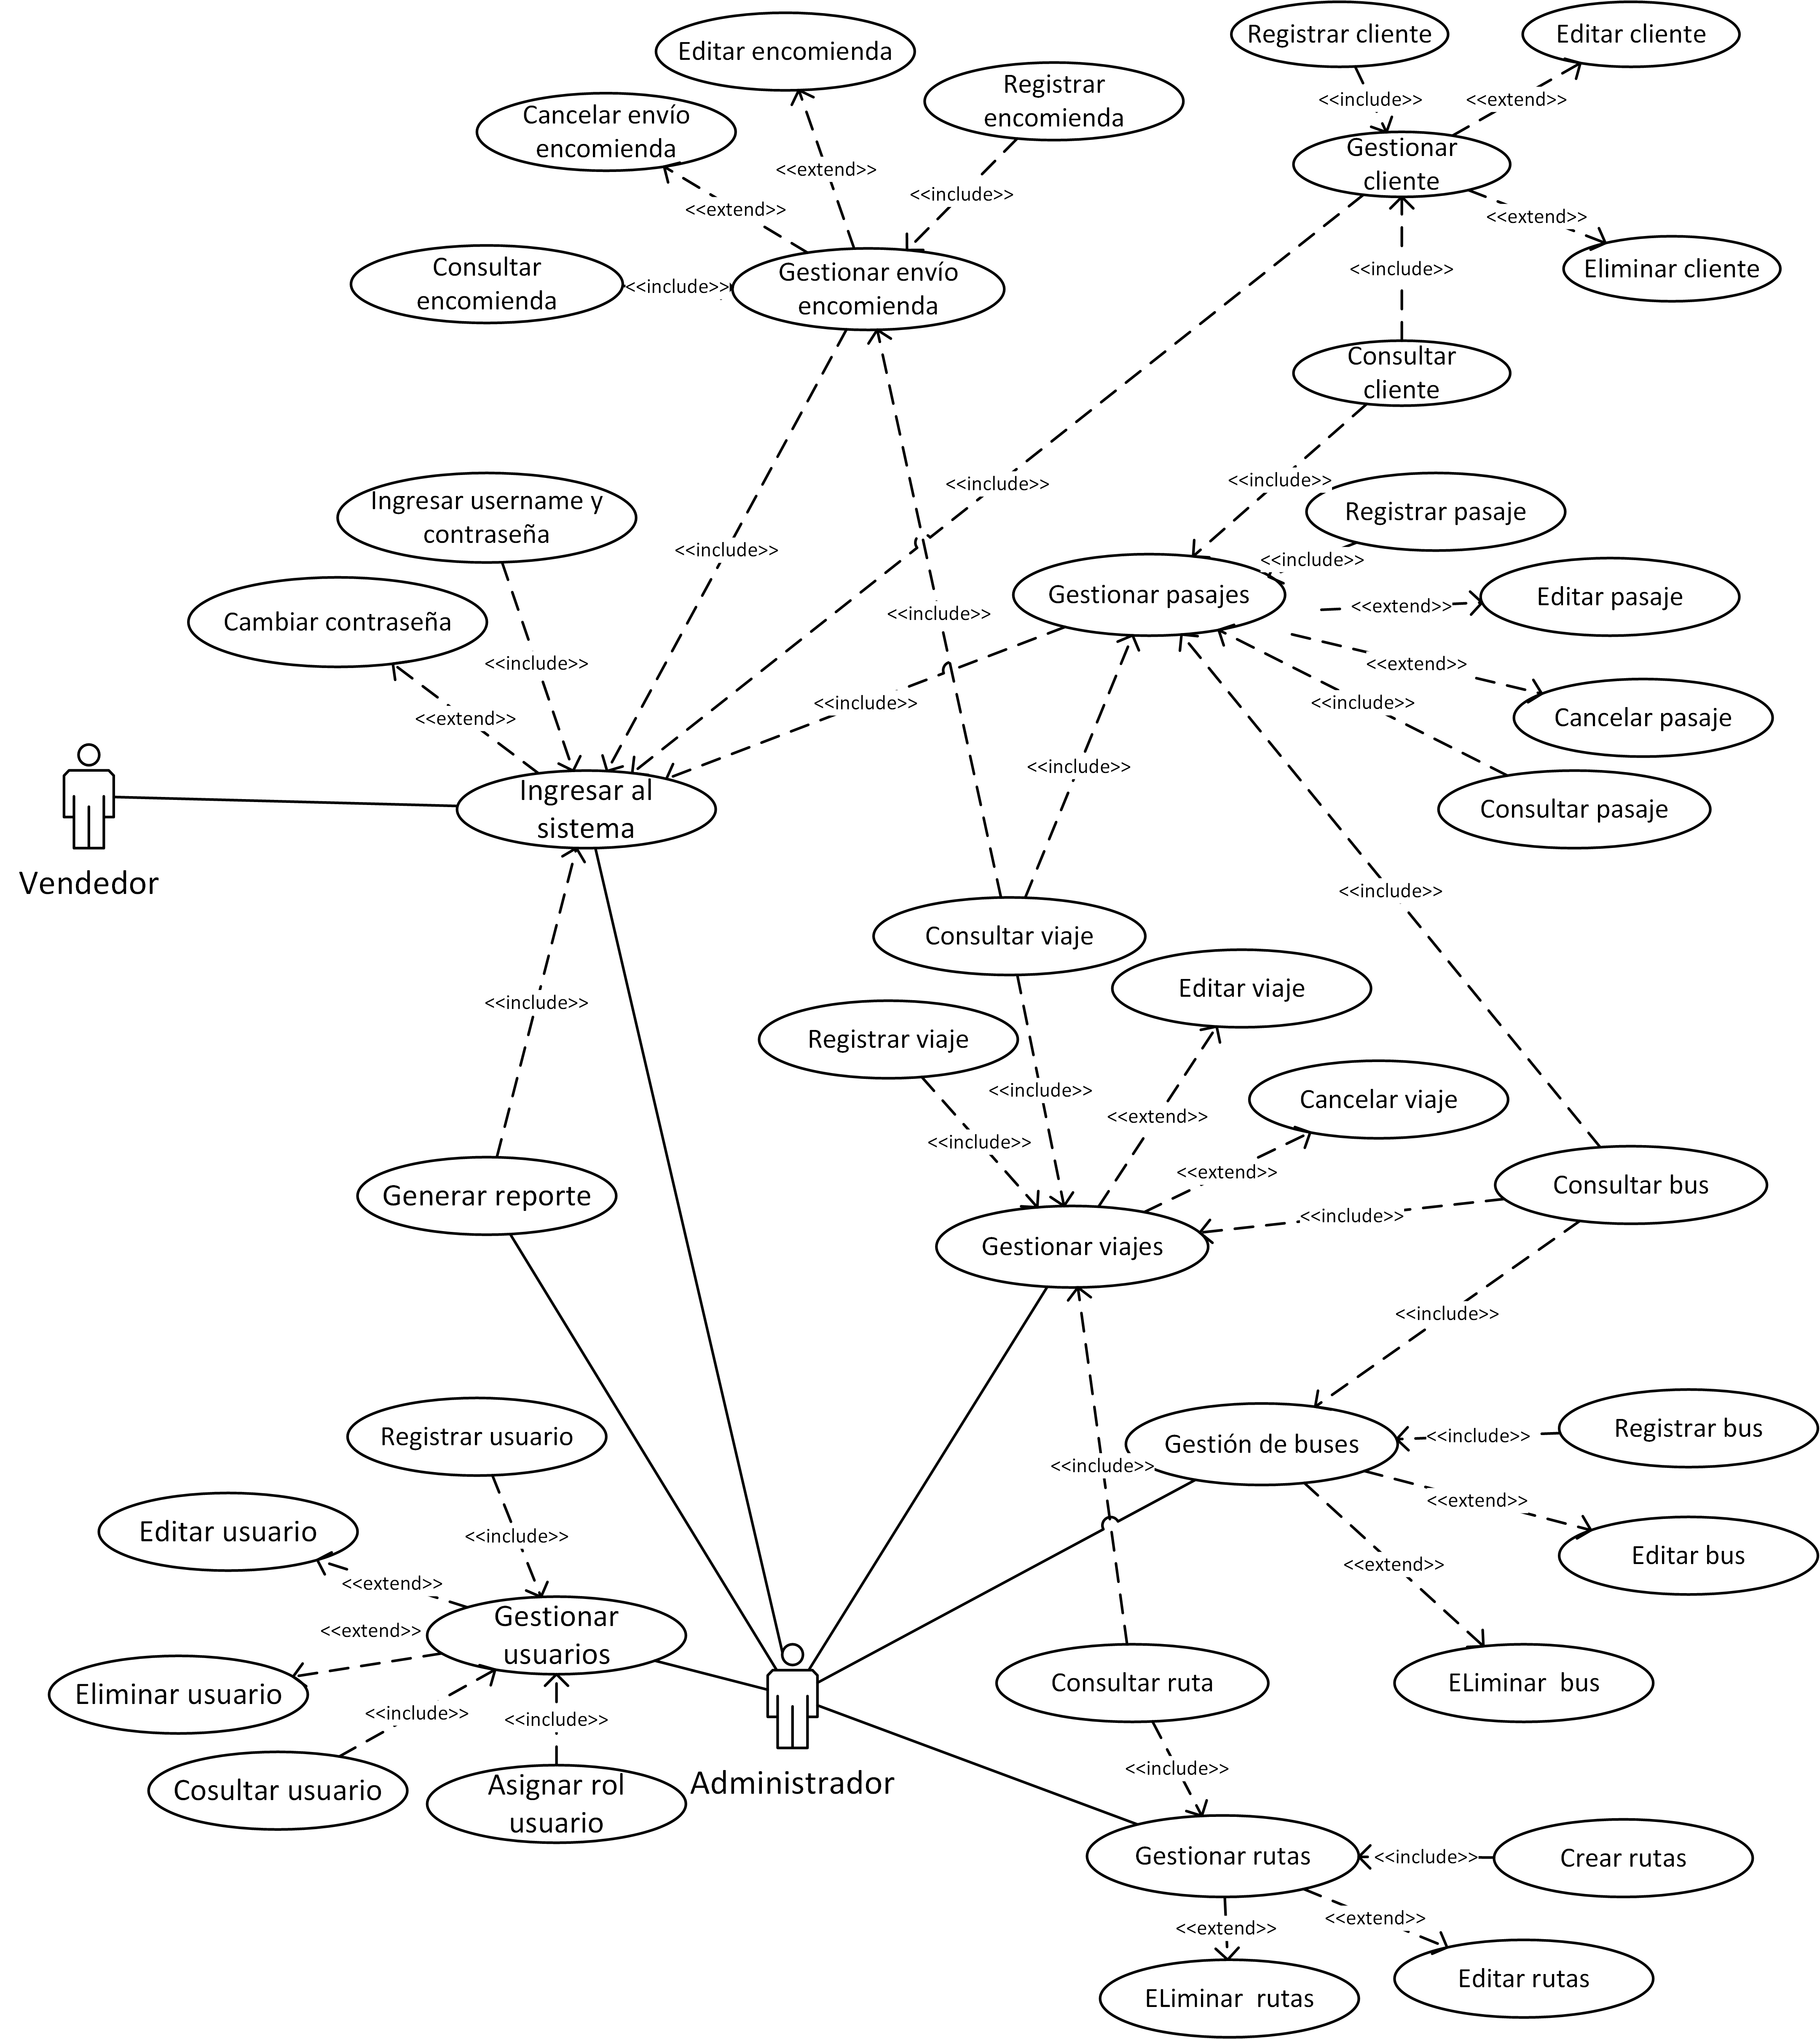
\includegraphics[width=0.9\textwidth]{imagenes/cap_3/casos_de_uso.png} % Inserta una imagen
		\vspace{0.3cm}
		\caption*{\textup{\textbf{Nota}: El diagrama representa los principales actores y casos de uso del sistema.}}
		\vspace{-0.8cm}
		\label{fig:caso_uso} % Etiqueta para referencia cruzada
	\end{figure}
	
	\noindent \textbf{Especificaciones de casos de uso}
	
	El presente apartado desde la tabla \ref{tab:tabla3_2} a la tabla \ref{tab:tabla3_10} contiene la especificación detallada de los casos de uso del sistema, organizados por módulos funcionales, para cada caso se describe el alcance, los objetivos específicos y las interacciones necesarias para completar las funcionalidades requeridas, proporcionando una visión clara del comportamiento esperado.
	
	\begingroup
	% \onehalfspacing
	
	\begin{longtable}{m{7.5cm}|m{7.5cm}}
		\caption[Especificación de casos de uso: Autenticación del usuario]{\newline Especificación de casos de uso: Autenticación del usuario} \label{tab:tabla3_2}\\
		\toprule
		\textbf{Caso de Uso:} Autenticación del usuario & \textbf{Actores:} Administrador, Personal de atención al cliente \\
		\midrule
		\endfirsthead
		
		\textbf{Caso de Uso:} Autenticación del usuario & \textbf{Actores:} Administrador, Personal de atención al cliente \\
		\midrule
		\endhead
		
		\bottomrule
		\endlastfoot
		
		\multicolumn{2}{m{15cm}}{\textbf{Descripción:} La página de autenticación de usuarios permite al administrador y al personal de atención al cliente acceder al sistema y realizar funciones de cada usuario.} \\ \hline
		
		\multicolumn{2}{m{15cm}}{\textbf{Secuencia Normal:}

			El usuario y la contraseña son validados en la base de datos.
			
			Se verifica en la base de datos el tipo de usuario que se ha autenticado y se lo dirige a las opciones pertinentes.
			
			Se visualizan las opciones que tiene cada usuario.
		} \\ \hline
		
		\textbf{Precondiciones:} El usuario debe contar con un nombre de usuario y una contraseña para poder acceder a las opciones del sistema web. & \textbf{Postcondiciones:} Los datos del usuario se mantienen mientras su sesión esté abierta después de que se ha autenticado en el sistema. \\ \hline
		
		\multicolumn{2}{m{15cm}}{\textbf{Excepciones:} Si el usuario y la contraseña no existen en la base de datos o si la contraseña no corresponde al usuario, se muestra una notificación de error.
		} \\
		
	\end{longtable}
	
	\endgroup
	 
	\vspace{-6pt}  % O el valor que necesites para ajustar
	% Nota personalizada fuera de `\caption*{}`
	\textbf{Nota}: Este caso de uso describe el proceso de autenticación de los usuarios.
	
\begingroup
% \onehalfspacing

	\begin{longtable}{m{7.5cm}|m{7.5cm}}
		\caption[Especificación de casos de uso: Gestionar bus]{\newline Especificación de casos de uso: Gestionar bus} \label{tab:tabla3_3}\\
		\toprule
		\textbf{Caso de Uso:} Gestionar bus & \textbf{Actores:} Administrador \\
		\midrule
		\endfirsthead
	
		\textbf{Caso de Uso:} Gestionar bus & \textbf{Actores:} Administrador \\
		\midrule
		\endhead
	
		\bottomrule
		\endlastfoot
	
		\multicolumn{2}{m{15cm}}{\textbf{Descripción:} Este caso de uso hace referencia al registro de los datos de un bus.} \\ \hline
	
		\multicolumn{2}{m{15cm}}{\textbf{Secuencia Normal:}
		
			El administrador debe elegir la opción “Configurar Bus” del ítem “Configurar”.
		
			El administrador debe consultar la existencia del bus a registrar.
		
			El administrador debe completar la placa del bus, la capacidad de personas, modelo y año.
		
			El administrador guarda el registro realizado.
		
			El administrador podrá editar los datos del registro y eliminar el registro realizado.
		} \\ \hline
	
		\textbf{Precondiciones:} El administrador debe acceder al sistema con su usuario y contraseña. & \textbf{Postcondiciones:} Ninguna. \\ \hline
	
		\multicolumn{2}{m{15cm}}{\textbf{Excepciones:}
		
			Si el usuario y la contraseña no existen en la base de datos o si la contraseña no corresponde al usuario, se muestra una notificación de error solicitando nuevamente los datos.
		
			De no completar los datos en los registros, se mostrará un mensaje mencionando qué datos están vacíos y cuáles no han sido seleccionados.
		} \\
	\end{longtable}
	\endgroup
	\vspace{-6pt}  % O el valor que necesites para ajustar
	% Nota personalizada fuera de `\caption*{}`
	\textbf{Nota}: El caso de uso cubre el proceso de registro de un bus en el sistema, incluyendo los detalles como la placa, capacidad, modelo y año, aso como la opción de editar o eliminar estos datos.

	
	\begingroup
	% \onehalfspacing
	
	\begin{longtable}{m{7.5cm}|m{7.5cm}}
		\caption[Especificación de casos de uso: Gestionar rutas]{\newline Especificación de casos de uso: Gestionar rutas} \label{tab:tabla3_4}\\
		\toprule
		\textbf{Caso de Uso:} Gestionar rutas & \textbf{Actores:} Administrador \\
		\midrule
		\endfirsthead
		
		\textbf{Caso de Uso:} Gestionar rutas & \textbf{Actores:} Administrador \\
		\midrule
		\endhead
		
		\bottomrule
		\endlastfoot
		
		\multicolumn{2}{m{15cm}}{\textbf{Descripción:} Este caso de uso hace referencia al registro de los lugares de origen y destino.} \\ \hline
		
		\multicolumn{2}{m{15cm}}{\textbf{Secuencia Normal:}
			
			El administrador debe elegir la opción “Registrar rutas” del ítem “Registro”.
			
			El administrador debe consultar la existencia de las rutas de origen y de destino a registrar.
			
			El administrador debe completar los datos del lugar de origen como el nombre de la ciudad. Por defecto el estado muestra como activo. De igual manera, el administrador deberá completar los mismos datos para el lugar de destino.
			
			El administrador guarda el registro realizado.
			
			El administrador podrá editar los datos del registro, eliminar el registro realizado y cambiar el estado del registro.
		} \\ \hline
		
		\textbf{Precondiciones:} El administrador debe acceder al sistema con su usuario y contraseña. & \textbf{Postcondiciones:} Ninguna. \\ \hline
		
		\multicolumn{2}{m{15cm}}{\textbf{Excepciones:}
			
			Si el usuario y la contraseña no existen en la base de datos o si la contraseña no corresponde al usuario, se muestra una notificación de error solicitando nuevamente los datos.
			
			De no completar los datos en los registros, se mostrará un mensaje mencionando qué datos están vacíos y cuáles no han sido seleccionados.
		} \\
	\end{longtable}
	\endgroup
	\vspace{-6pt}  % O el valor que necesites para ajustar
	% Nota personalizada fuera de `\caption*{}`
	\textbf{Nota}: Este caso de uso se refiere al registro de rutas, en el cual el administrador debe ingresar los lugares de origen y destino, con la opción de editar o eliminar estos registros posteriormente.	
	
	\begingroup
	% \onehalfspacing	
	\begin{longtable}{m{7.5cm}|m{7.5cm}}
		\caption[Especificación de casos de uso: Gestionar viajes]{\newline Especificación de casos de uso: Gestionar viajes} \label{tab:tabla3_5}\\
		\toprule
		\textbf{Caso de Uso:} Gestionar viajes & \textbf{Actores:} Administrador \\
		\midrule
		\endfirsthead
		
		\textbf{Caso de Uso:} Gestionar viajes & \textbf{Actores:} Administrador \\
		\midrule
		\endhead
		
		\bottomrule
		\endlastfoot
		
		\multicolumn{2}{m{15cm}}{\textbf{Descripción:} Este caso de uso hace referencia a la programación de los viajes con sus fechas respectivas para cada uno. Se asignará un viaje a un bus y, por defecto, se indicarán los lugares de origen y destino. Tendrá un estado de viaje.} \\ \hline
		
		\multicolumn{2}{m{15cm}}{\textbf{Secuencia Normal:}
			
			El administrador debe elegir la opción “Registrar viajes” del ítem “Registro”.
			
			El administrador debe consultar el bus que realizará un viaje.
			
			El sistema muestra el lugar de ubicación del bus y por defecto lo asigna al campo de ciudad de origen. También se completan los campos de capacidad de personas y límite de carga.
			
			El administrador debe completar la ciudad de destino, debe programar la fecha de salida y de llegada del viaje. Debe elegir un estado del viaje que, por defecto, el sistema muestra como PENDIENTE.
			
			El administrador guarda el registro realizado.
			
			El administrador podrá editar los datos del registro y eliminar el registro realizado.
		} \\ \hline
		
		\textbf{Precondiciones:} El administrador debe acceder al sistema con su usuario y contraseña. & \textbf{Postcondiciones:} Ninguna. \\ \hline
		
		\multicolumn{2}{m{15cm}}{\textbf{Excepciones:} De no completar los datos en los registros, se mostrará un mensaje mencionando qué datos están vacíos y cuáles no han sido seleccionados.
		} \\
	\end{longtable}
	\endgroup
	\vspace{-6pt}  % O el valor que necesites para ajustar
	% Nota personalizada fuera de `\caption*{}`
	\textbf{Nota}: Este caso de uso trata sobre la programación de viajes, donde el administrador asigna un bus y establece la fecha y hora de salida.
	
	\begingroup
	% \onehalfspacing
	\begin{longtable}{m{7.5cm}|m{7.5cm}}
		\caption[Especificación de casos de uso: Gestionar venta y reserva de pasaje]{\newline Especificación de casos de uso: Gestionar pasaje} \label{tab:tabla3_6}\\
		\toprule
		\textbf{Caso de Uso:} Gestionar venta y reserva de pasajes & \textbf{Actores:} Personal de atención al cliente \\
		\midrule
		\endfirsthead
		\endhead
		\bottomrule
		\endlastfoot
		\multicolumn{2}{m{15cm}}{\textbf{Descripción:} Este caso de uso hace referencia a la venta y reservas de pasajes para los buses.} \\ \hline
		
		\multicolumn{2}{m{15cm}}{\textbf{Secuencia Normal:}
			
			El vendedor debe elegir la opción “Pasajes”.
			
			El vendedor consulta el día del viaje, el sistema mostrará la lista de viajes programados según la fecha actual del sistema. Por defecto se completan los datos de la ciudad de origen y de destino y el bus programado.
			
			El vendedor debe consultar los asientos libres en los buses disponibles.
			
			El vendedor consulta la existencia del cliente; si existe, se obtienen los datos y se completan en los campos vacíos; si no existe, procede a registrar los datos del cliente.
			
			Por defecto se completan los datos en los demás campos según el registro de los datos de las personas. El sistema consulta, calcula el monto del pago y completa los campos.
			
			Se imprime el boleto del pasaje con los datos del pasajero, el destino, el monto de pago, el tipo de pasaje y un número de ticket.
			
			El vendedor también podrá editar los datos del registro del pasaje y cancelar el registro.
		} \\ \hline
		
		\textbf{Precondiciones:} El vendedor debe acceder al sistema con su usuario y contraseña. & \textbf{Postcondiciones:} Ninguna. \\ \hline
		
		\multicolumn{2}{m{15cm}}{\textbf{Excepciones:} De no completar los datos en los registros, se mostrará un mensaje mencionando qué datos están vacíos y cuáles no han sido seleccionados.
		} \\
		
	\end{longtable}
	\endgroup 
	\vspace{-20pt}  % O el valor que necesites para ajustar
	% Nota personalizada fuera de `\caption*{}`
	\textbf{Nota}: Este caso de uso describe el proceso de venta y reserve de pasajes, incluyendo la consulta de disponibilidad, registro de datos del cliente y emisión del boleto.
	
	\begingroup
	% \onehalfspacing
	
	\begin{longtable}{m{7.5cm}|m{7.5cm}}
		\caption[Especificación de casos de uso: Gestionar rol de usuario]{\newline Especificación de casos de uso: Gestionar rol de usuario} \label{tab:tabla3_9}\\
		\toprule
		\textbf{Caso de Uso:} Gestionar rol de usuario & \textbf{Actores:} Administrador \\
		\midrule
		\endfirsthead
		\endhead
		\bottomrule
		\endlastfoot
		
		\multicolumn{2}{m{15cm}}{\textbf{Descripción:} Este caso de uso hace referencia al registro de un rol de usuario.} \\ \hline
		
		\multicolumn{2}{m{15cm}}{\textbf{Secuencia Normal:}
			
			El administrador debe elegir la opción “Configurar roles”.
			
			El administrador debe consultar la existencia del rol a registrar.
			
			El administrador debe completar los campos de nombre del rol y registrar una descripción del mismo.
			
			El administrador debe seleccionar los accesos que tendrá el rol al sistema.
			
			El administrador podrá editar los datos del registro y eliminar el registro realizado.
		} \\ \hline
		
		\textbf{Precondiciones:} El administrador debe acceder al sistema con su usuario y contraseña. & \textbf{Postcondiciones:} Ninguna. \\ \hline
		
		\multicolumn{2}{m{15cm}}{\textbf{Excepciones:} De no completar los datos en los registros, se mostrará un mensaje mencionando qué datos están vacíos y cuáles no han sido seleccionados.
		} \\
	\end{longtable}
	\endgroup
	\vspace{-6pt}  % O el valor que necesites para ajustar
	% Nota personalizada fuera de `\caption*{}`
	\textbf{Nota}: Caso de uso que describe el proceso de asignación de roles a los usuarios del sistema.
		
	\begingroup
	% \onehalfspacing
	\begin{longtable}{m{7.5cm}|m{7.5cm}}
		\caption[Especificación de casos de uso: Gestionar encomienda]{\newline Especificación de casos de uso: Gestionar encomienda} \label{tab:tabla3_8}\\
		\toprule
		\textbf{Caso de Uso:} Gestionar encomienda & \textbf{Actores:} Personal de atención al cliente \\
		\midrule
		\endfirsthead
		\endhead
		\bottomrule
		\endlastfoot
		\multicolumn{2}{m{15cm}}{\textbf{Descripción:} Este caso de uso hace referencia al registro de las encomiendas.} \\ \hline
		
		\multicolumn{2}{m{15cm}}{\textbf{Secuencia Normal:}
			
			El recepcionista debe elegir la opción “Enviar encomienda”.
			
			El recepcionista debe consultar el día del viaje. Por defecto se completan los campos del lugar de origen y destino y el bus programado.
			
			El recepcionista realiza una consulta de la existencia de los clientes (remitente y destinatario); si existen se obtienen los datos y se completan los campos vacíos. Si no existen, se procede a registrar sus datos.
			
			El recepcionista debe registrar los datos de la encomienda o carga, llenar una descripción de la encomienda, la cantidad, el peso y el monto a pagar. El estado del encargo por defecto se guarda como “PENDIENTE”.
			
			El recepcionista debe imprimir el comprobante del registro del envío.
			
			Cuando la encomienda llega a su destino y se realiza el recojo, el recepcionista debe constatar que la persona que recoge sea la registrada en el sistema. Luego debe actualizar el estado del encargo a “ENTREGADO” y hacer entrega de la encomienda.
		} \\ \hline
		
		\textbf{Precondiciones:} El recepcionista debe acceder al sistema con su usuario y contraseña. & \textbf{Postcondiciones:} Ninguna. \\ \hline
		
		\multicolumn{2}{m{15cm}}{\textbf{Excepciones:} De no completar los datos en los registros, se mostrará un mensaje mencionando qué datos están vacíos y cuáles no han sido seleccionados.
			
		De no actualizar el estado del encargo entregado, éste se mantendrá como pendiente.
		} \\
	\end{longtable}
	\endgroup
	\vspace{-18pt}  % O el valor que necesites para ajustar
	% Nota personalizada fuera de `\caption*{}`
	\textbf{Nota}: Caso de uso que hace referencia al registro y gestión de encomiendas.
	
	\begingroup
	% \onehalfspacing
	
	\begin{longtable}{m{7.5cm}|m{7.5cm}}
		\caption[Especificación de casos de uso: Generar reporte]{\newline Especificación de casos de uso: Generar reporte} \label{tab:tabla3_10}\\
		\toprule
		\textbf{Caso de Uso:} Generar reporte & \textbf{Actores:} Administrador, personal de atención al cliente \\
		\midrule
		\endfirsthead
		\endhead		
		\bottomrule
		\endlastfoot
		
		\multicolumn{2}{m{15cm}}{\textbf{Descripción:} Este caso de uso hace referencia al proceso de generación de reportes necesarios para la gestión administrativa de la empresa.} \\ \hline
		
		\multicolumn{2}{m{15cm}}{\textbf{Secuencia Normal:}
			
			El usuario puede ver dentro del sistema sólo los reportes que su perfil le permita. Cabe mencionar que el perfil con todos los permisos u opciones es el del Administrador.
			
			El usuario selecciona el reporte que desea generar.
			
			El usuario ingresa los parámetros de búsqueda antes de generar el reporte.
			
			El sistema muestra los datos del reporte.
			
			El sistema imprime el reporte seleccionado.
		} \\ \hline
		
		\textbf{Precondiciones:} Los usuarios deben acceder al sistema con su usuario y contraseña. & \textbf{Postcondiciones:} Ninguna. \\ \hline
		
		\multicolumn{2}{m{15cm}}{\textbf{Excepciones:} Si el usuario y la contraseña no existen o si la contraseña no corresponde al usuario, se muestra una notificación de error solicitando nuevamente los datos.
		} \\
		
	\end{longtable}
	\endgroup
	\vspace{-18pt}  % O el valor que necesites para ajustar
	% Nota personalizada fuera de `\caption*{}`
	\textbf{Nota}: Caso de uso que describe el procedimiento para la generación de reportes.
		
	\subsection{Especificación de requerimientos}
	En esta etapa del proyecto, se presenta la especificación detallada de los requerimientos funcionales y no funcionales identificados para el sistema. Esta sección tiene como objetivo proporcionar una descripción completa de las capacidades y restricciones que deberá cumplir la solución, estableciendo así las bases para su posterior diseño e implementación.\\	
	\textbf{Requerimientos funcionales}
	\begingroup
	%\onehalfspacing	
	\begin{longtable}{m{1.5cm}|m{14cm}}
		\caption[Lista de Requerimientos Funcionales]{\newline Lista de Requerimientos Funcionales} \label{tab:tabla_requerimientos_funcionales}\\
		\toprule
		\textbf{ID} & \textbf{Requerimiento} \\
		\midrule
		\endfirsthead		
		\bottomrule
		\endlastfoot
		
		RF-01 & El sistema contará con un módulo de gestión de perfiles de usuarios, distinguiendo entre administradores y empleados. \\
		RF-02 & El sistema permitirá la gestión de rutas y horarios de los servicios de transporte. \\
		RF-03 & El sistema contará con un módulo de venta y reserva de pasajes para los usuarios. \\
		RF-04 & El sistema realizará la asignación de asientos en los vehículos de transporte. \\
		RF-05 & El sistema permitirá el registro de las encomiendas transportadas. \\
		RF-06 & El sistema gestionará la flota de buses, incluyendo información de los vehículos y conductores. \\		
	\end{longtable}	
	\endgroup
	\vspace{-18pt}  % O el valor que necesites para ajustar
	% Nota personalizada fuera de `\caption*{}`
	\textbf{Nota}: Esta tabla enumera los principales requerimientos funcionales del sistema propuesto, abarcando aspectos relacionados con usuarios, servicios de transporte, ventas y operaciones logísticas.\\		
	\textbf{Requerimientos no funcionales} \\	
	\begingroup
	%\onehalfspacing
	\begin{longtable}{m{1.4cm} m{14.5cm}}
		\caption[Lista de Requerimientos No Funcionales]{\newline Lista de Requerimientos No Funcionales} \label{tab:tabla_requerimientos_nofuncionales}\\
		\toprule
		\textbf{ID} & \textbf{Requerimiento} \\
		\midrule
		\endfirsthead		
		\bottomrule
		\endlastfoot
		
		RNF-01 & El sistema debe ser accesible desde múltiples navegadores (Chrome, Firefox) y celulares. \\
		RNF-02 & Capacidad de exportar reportes en formatos estándar (PDF, CSV, Excel). \\
		RNF-03 & Arquitectura de software modular y escalable para facilitar actualizaciones. \\
		
	\end{longtable}
	\endgroup
	
	\vspace{-18pt}
	\textbf{Nota}: Esta tabla enumera los principales requerimientos no funcionales del sistema.
		
	\subsection{Gestión de requerimientos}
	En esta etapa del proyecto, se presentan los diagramas de actividades que se utilizan para representar los flujos de trabajo relacionados con el manejo y control de los requerimientos. 
	
	%A continuación, en las figuras \ref{fig:DA_ingreso}, \ref{fig:DA_registro}, \ref{fig:DA_pasajes} y \ref{fig:DA_encomiendas}, se muestran los diagramas de actividades correspondientes.

	%\vspace{0.05cm} % Agregar 1 cm de espacio entre el párrafo y la figura
	
	\begin{figure}[!h] % 'H' del paquete 'float' para mantener posición	
		\caption[Diagrama de actividades - Ingresar al sistema]
		{\newline Diagrama de actividades del proceso de ingreso al sistema.} % Leyenda en la parte superior
		\centering
		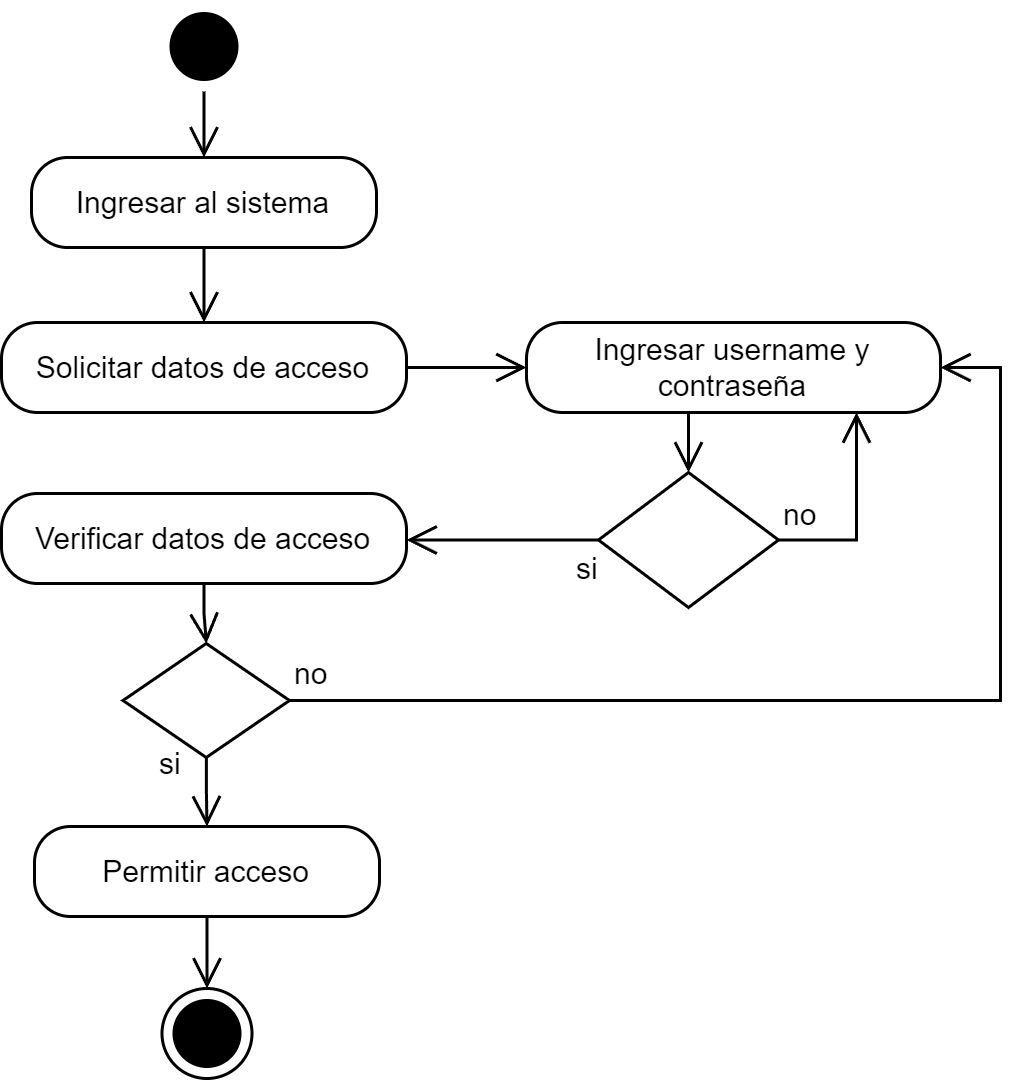
\includegraphics[width=0.45\textwidth]{imagenes/cap_3/ingreso.drawio.png} % Inserta una imagen
		
		\begin{flushleft}
		\begin{doublespace}
			\hspace{1.20cm} \textbf{Nota.} El diagrama describe el flujo de actividades que realiza el usuario para iniciar sesión en el sistema. % Nota al pie para esta figura
		\end{doublespace}
		\end{flushleft}
		\vspace{-16pt}
		\label{fig:DA_ingreso} % Etiqueta para referencia cruzada
	\end{figure}

	\vspace{0.3cm} % Agregar 1 cm de espacio entre el párrafo y la figura
	
	\begin{figure}[!h] % 'H' del paquete 'float' para mantener posición	
		\caption[Diagrama de actividades - Venta y reserva de pasajes]
		{\newline Diagrama de actividades del proceso de venta y reserva de pasajes.} % Leyenda en la parte superior
		\centering
		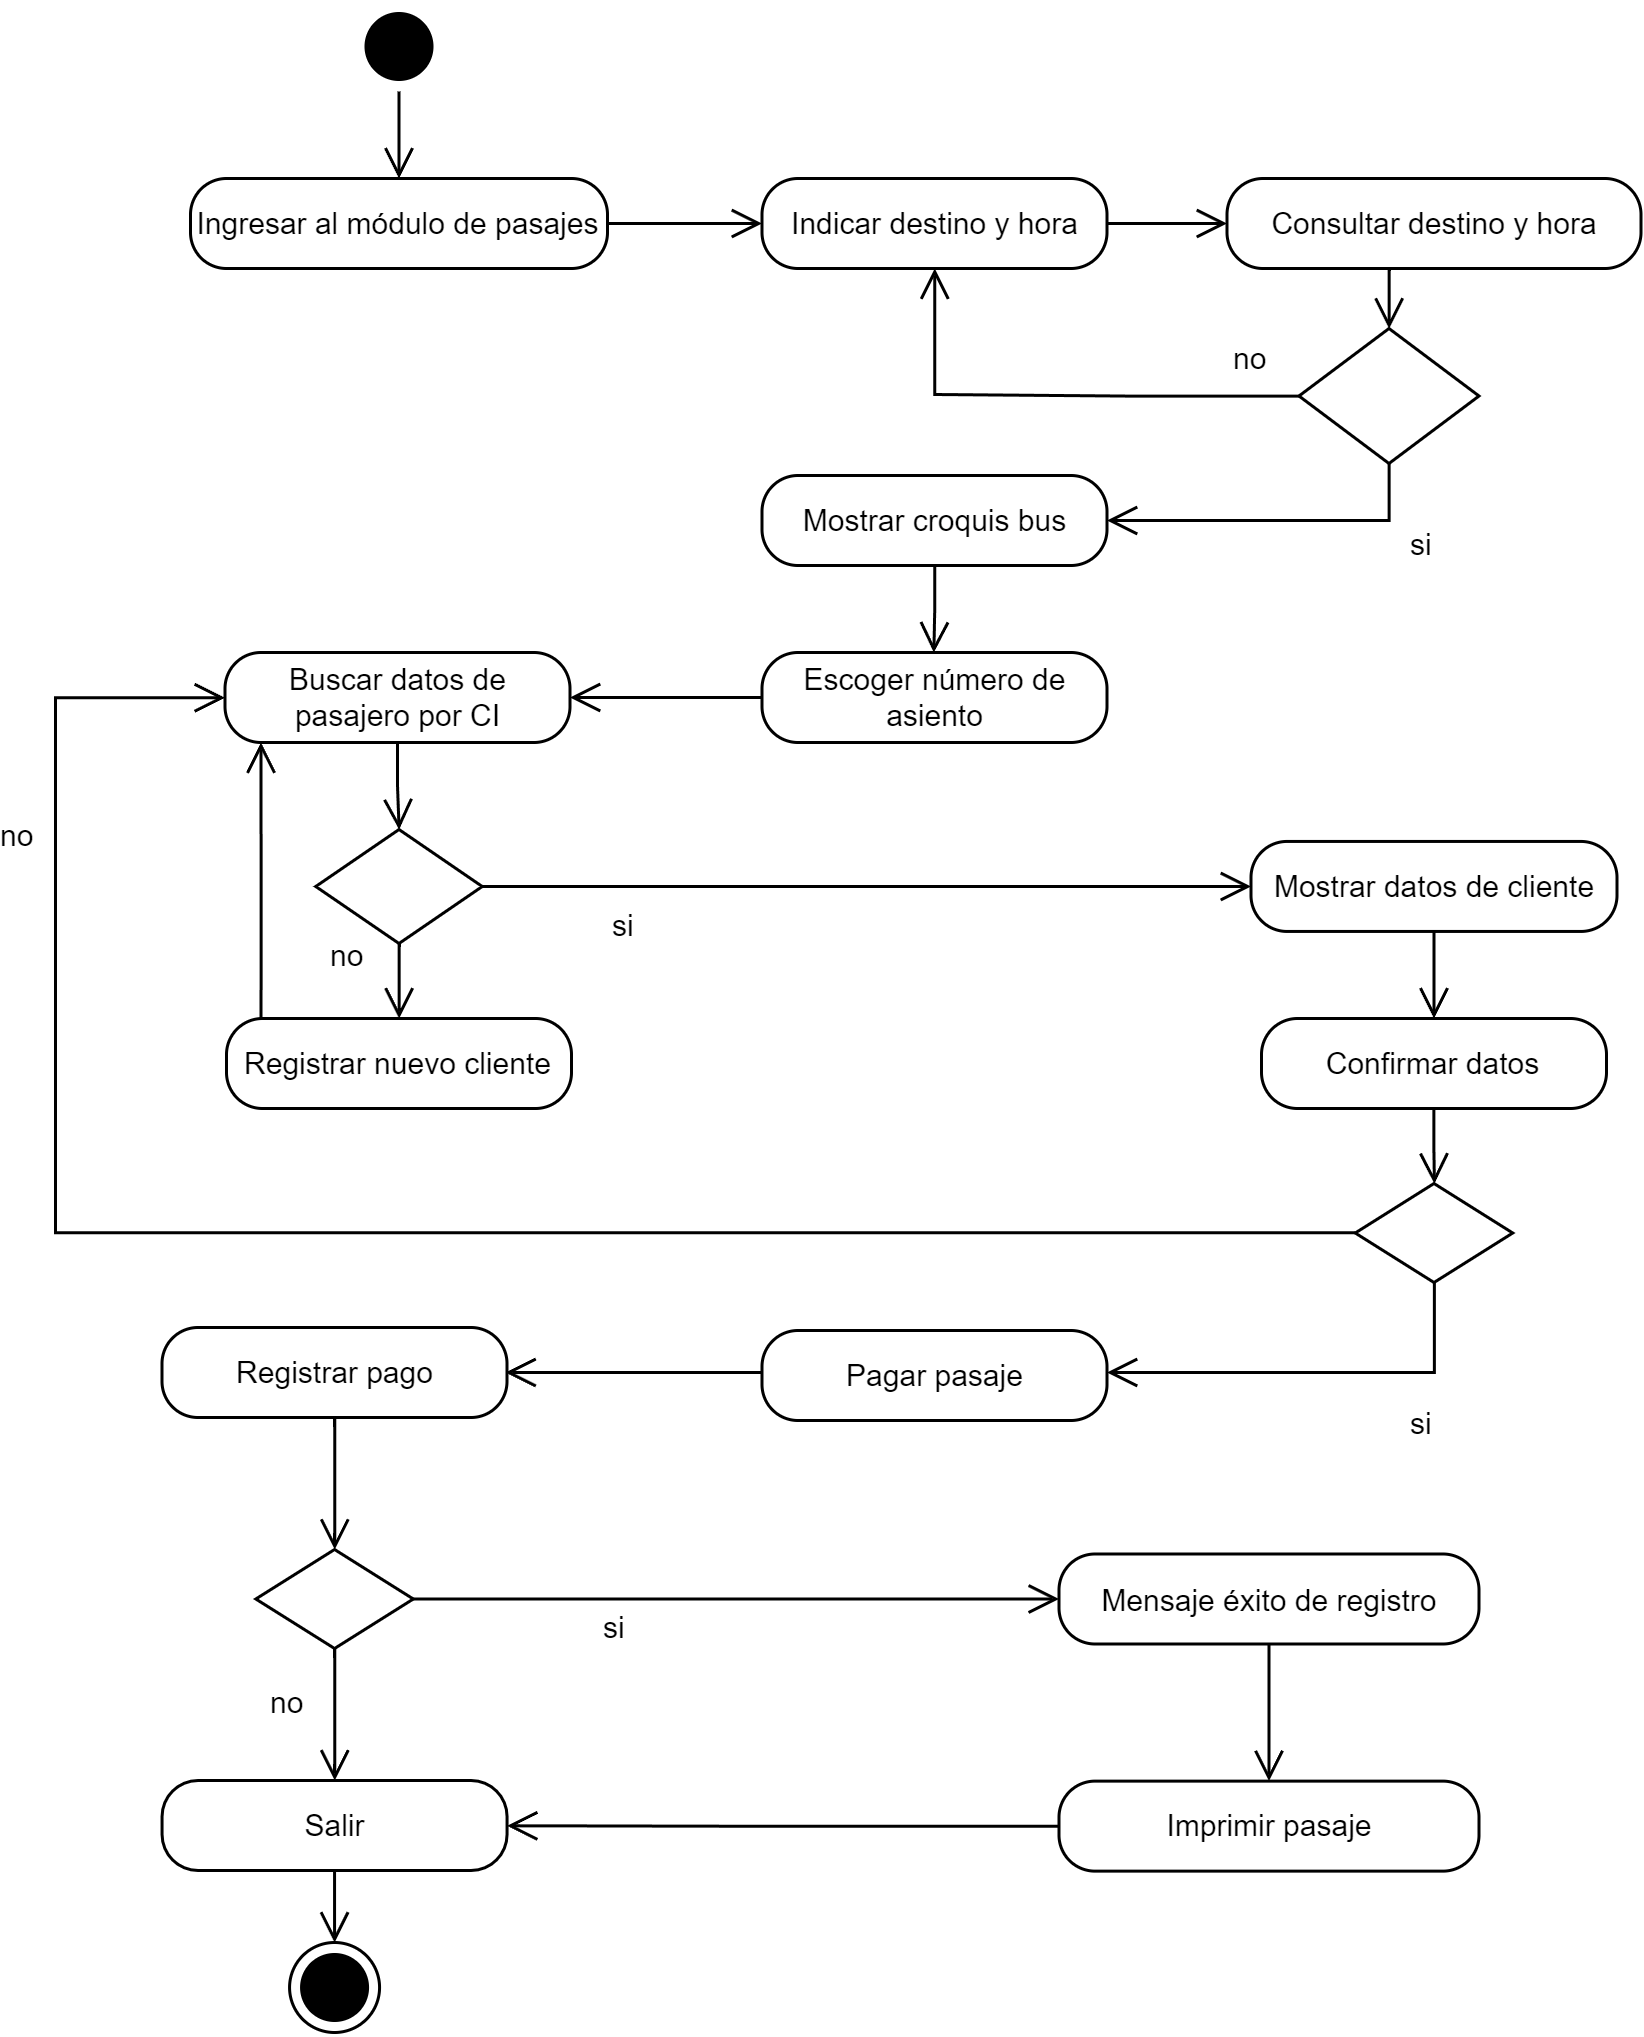
\includegraphics[width=0.85\textwidth]{imagenes/cap_3/pasaje.drawio.png} % Inserta una imagen
		\begin{flushleft}
		\begin{doublespace}
			\hspace{1.20cm} \textbf{Nota.} El diagrama muestra el flujo de actividades desde el ingreeso al módulo de venta - reserva de pasajes hasta la confirmacion de la venta o reserva. % Nota al pie para esta figura
		\end{doublespace}
		\end{flushleft}
		\vspace{-16pt}
		\label{fig:DA_pasajes} % Etiqueta para referencia cruzada
	\end{figure}
	
	\vspace{0.3cm} % Agregar 1 cm de espacio entre el párrafo y la figura
	
	\begin{figure}[!h] % 'H' del paquete 'float' para mantener posición	
		\caption[Diagrama de actividades - Registro de encomiendas]
		{\newline Diagrama de actividades del proceso de registro del envío de encomiendas.} % Leyenda en la parte superior
		\centering
		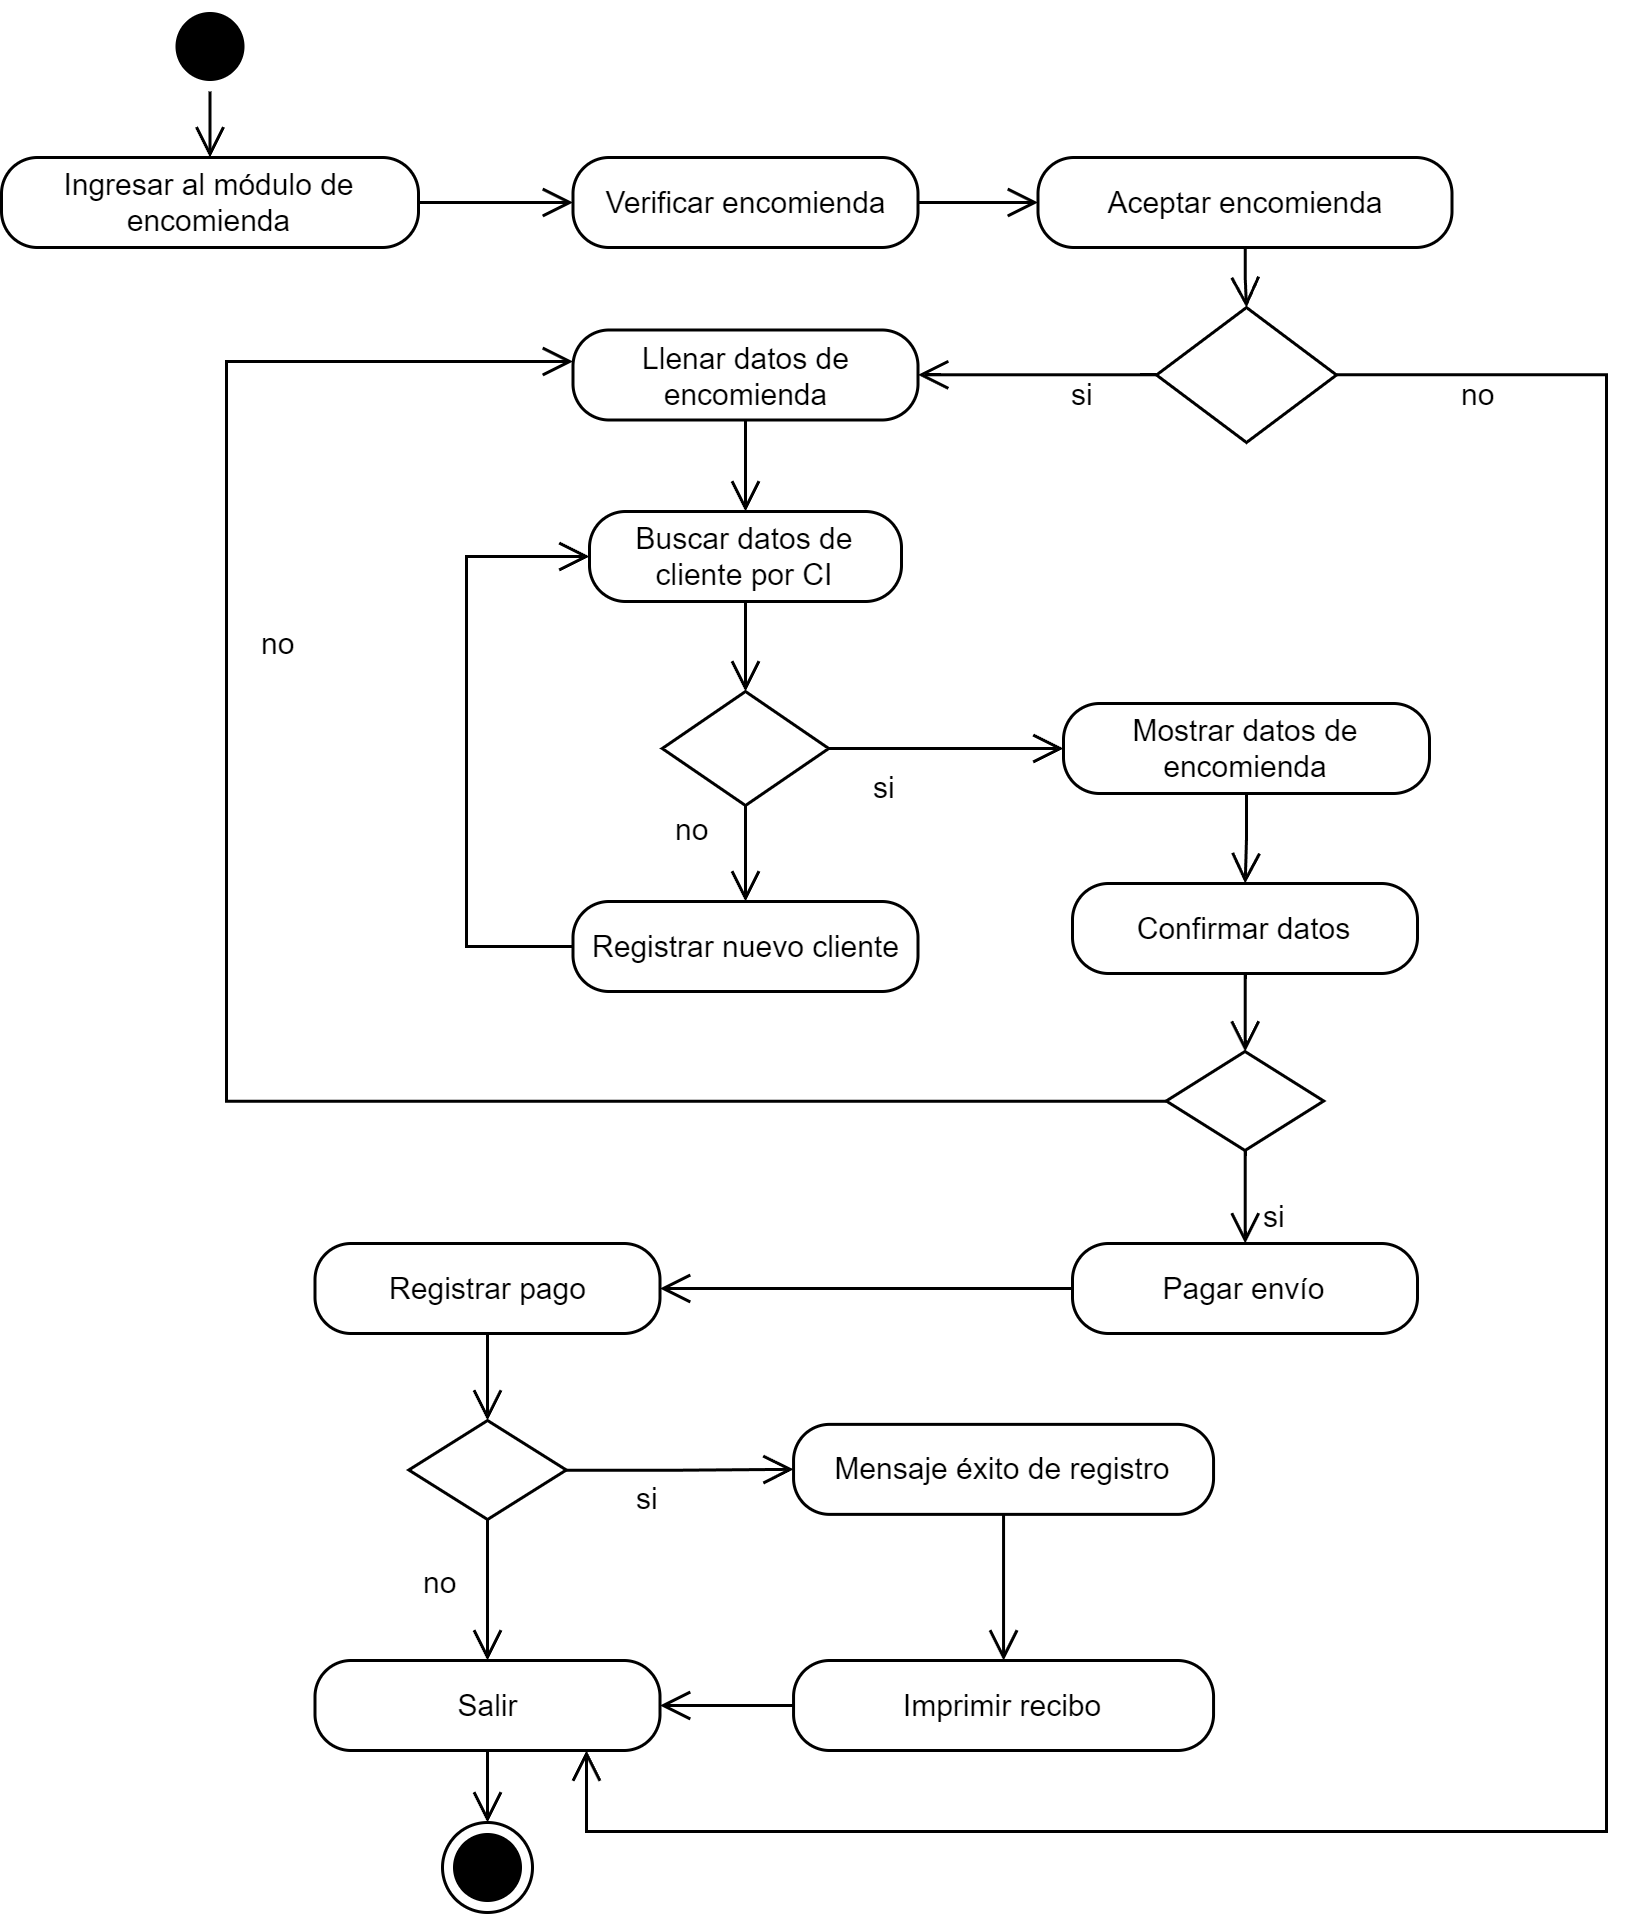
\includegraphics[width=0.9\textwidth]{imagenes/cap_3/encomiendas.drawio.png} % Inserta una imagen
		
		\begin{flushleft}
		\begin{doublespace}
			\hspace{1.20cm} \textbf{Nota.} El diagrama representa las acciones necesarias para registrar una encomienda. % Nota al pie para esta figura
		\end{doublespace}
		\end{flushleft}
		\vspace{-16pt}
		\label{fig:DA_encomiendas} % Etiqueta para referencia cruzada
	\end{figure}
	
	\vspace{0.3cm} % Agregar 1 cm de espacio entre el párrafo y la figura
	
	\begin{figure}[!h] % 'H' del paquete 'float' para mantener posición	
		\caption[Diagrama de actividades - Registro de personal]
		{\newline Diagrama de actividades del proceso de registro de personal - clientes.} % Leyenda en la parte superior
		\centering
		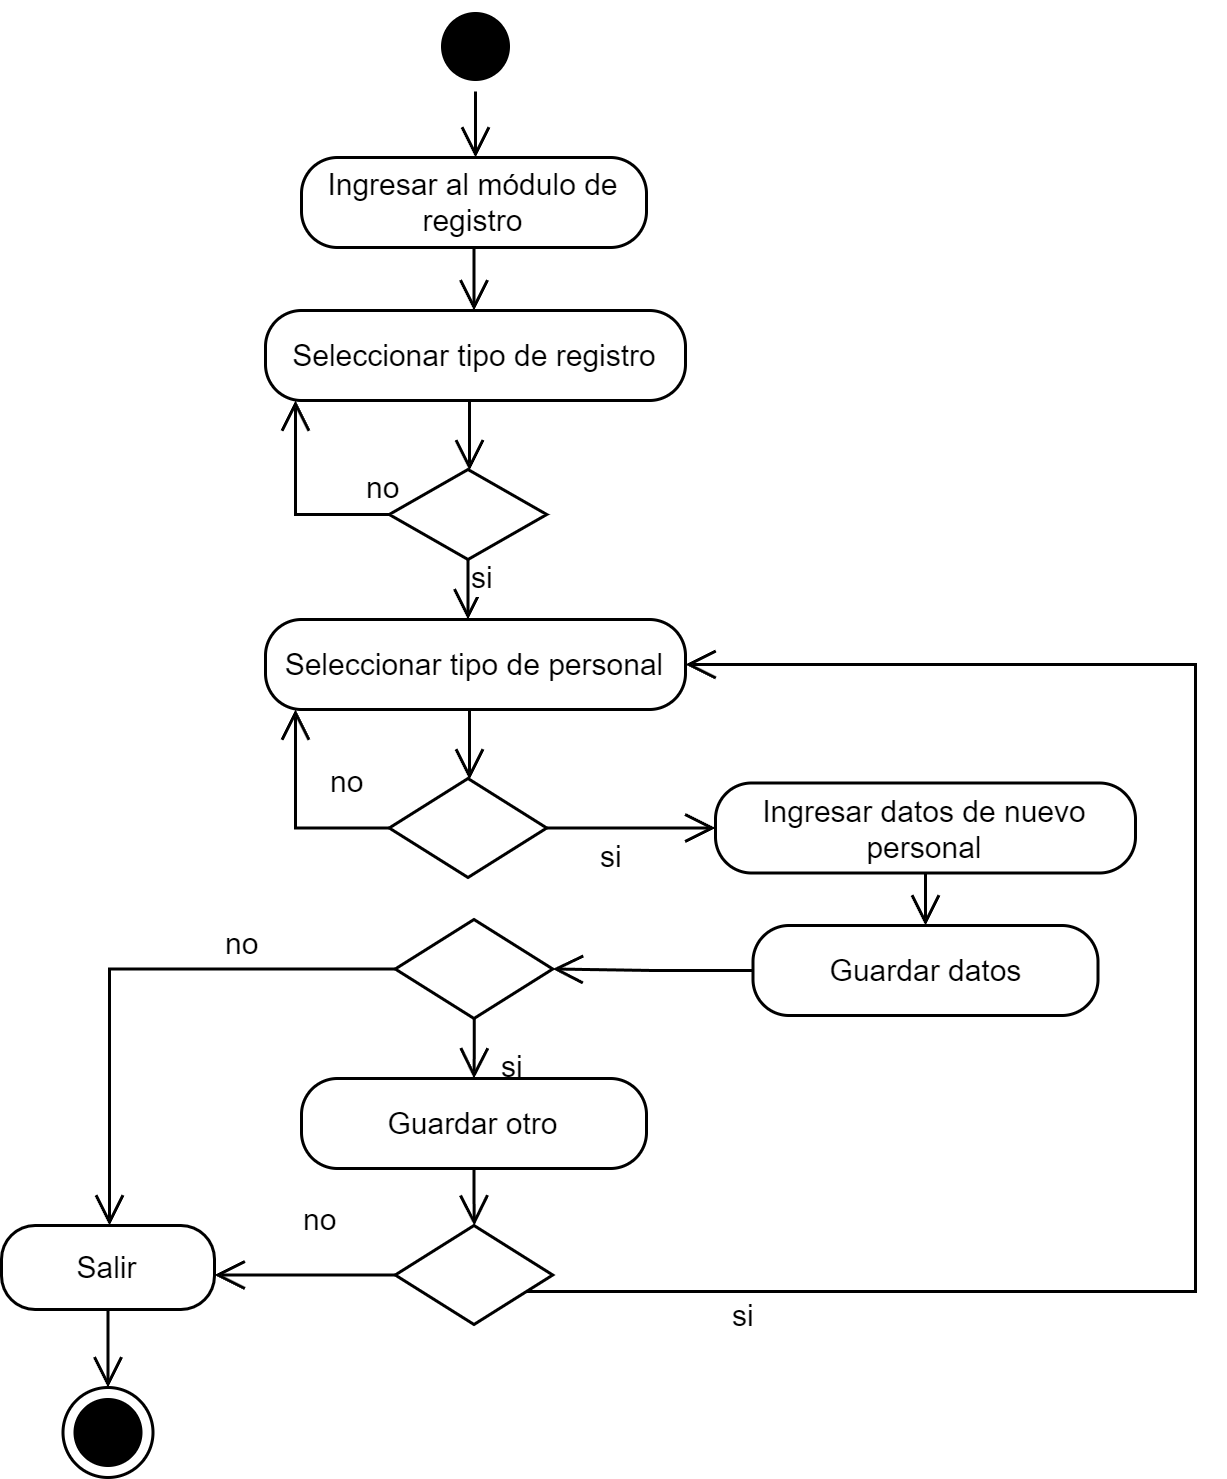
\includegraphics[width=0.5\textwidth]{imagenes/cap_3/registro.drawio.png} % Inserta una imagen
		
		\begin{flushleft}
			\begin{doublespace}
			\hspace{1.20cm} \textbf{Nota.} El diagrama describe las actividades requeridas para registrar en el sistema a los usarios, tanto personal administrativo como clientes. % Nota al pie para esta figura
			\end{doublespace}
		\end{flushleft}
		\vspace{-40pt} % hace que se acerque mas el texto
		\label{fig:DA_registro} % Etiqueta para referencia cruzada
	\end{figure}
	
	En las figuras \ref{fig:DA_ingreso}, \ref{fig:DA_pasajes}, \ref{fig:DA_encomiendas}, y \ref{fig:DA_registro}, se muestran los diagramas de actividades con los flujos correspondientes a cada actividad.

\section{DISEÑO DEL SISTEMA Y DEL SOFTWARE}
	Para el modelado de datos ahora se procede a realizar el modelo entidad - relación que permite visualizar la estructura inicial de la base de datos.
	\subsection{Diagrama entidad - relación}
	A continuación en la figura \ref{fig:ent_atri} se muestran las entidades del sistema, cada entidad se representa con sus atributos específicos, se distinguen las claves primarias y los atributos descriptivos, estableciendo así la base para el almacenamiento de la información del sistema.
	
	\begin{figure}[!h] % 'H' del paquete 'float' para mantener posición	
		\caption[Diagrama Entidad-Relación ]
		{\newline Diagrama Entidad-Relación (Entidades y atributos)} % Leyenda en la parte superior
		\vspace{0.3cm}
		\centering
		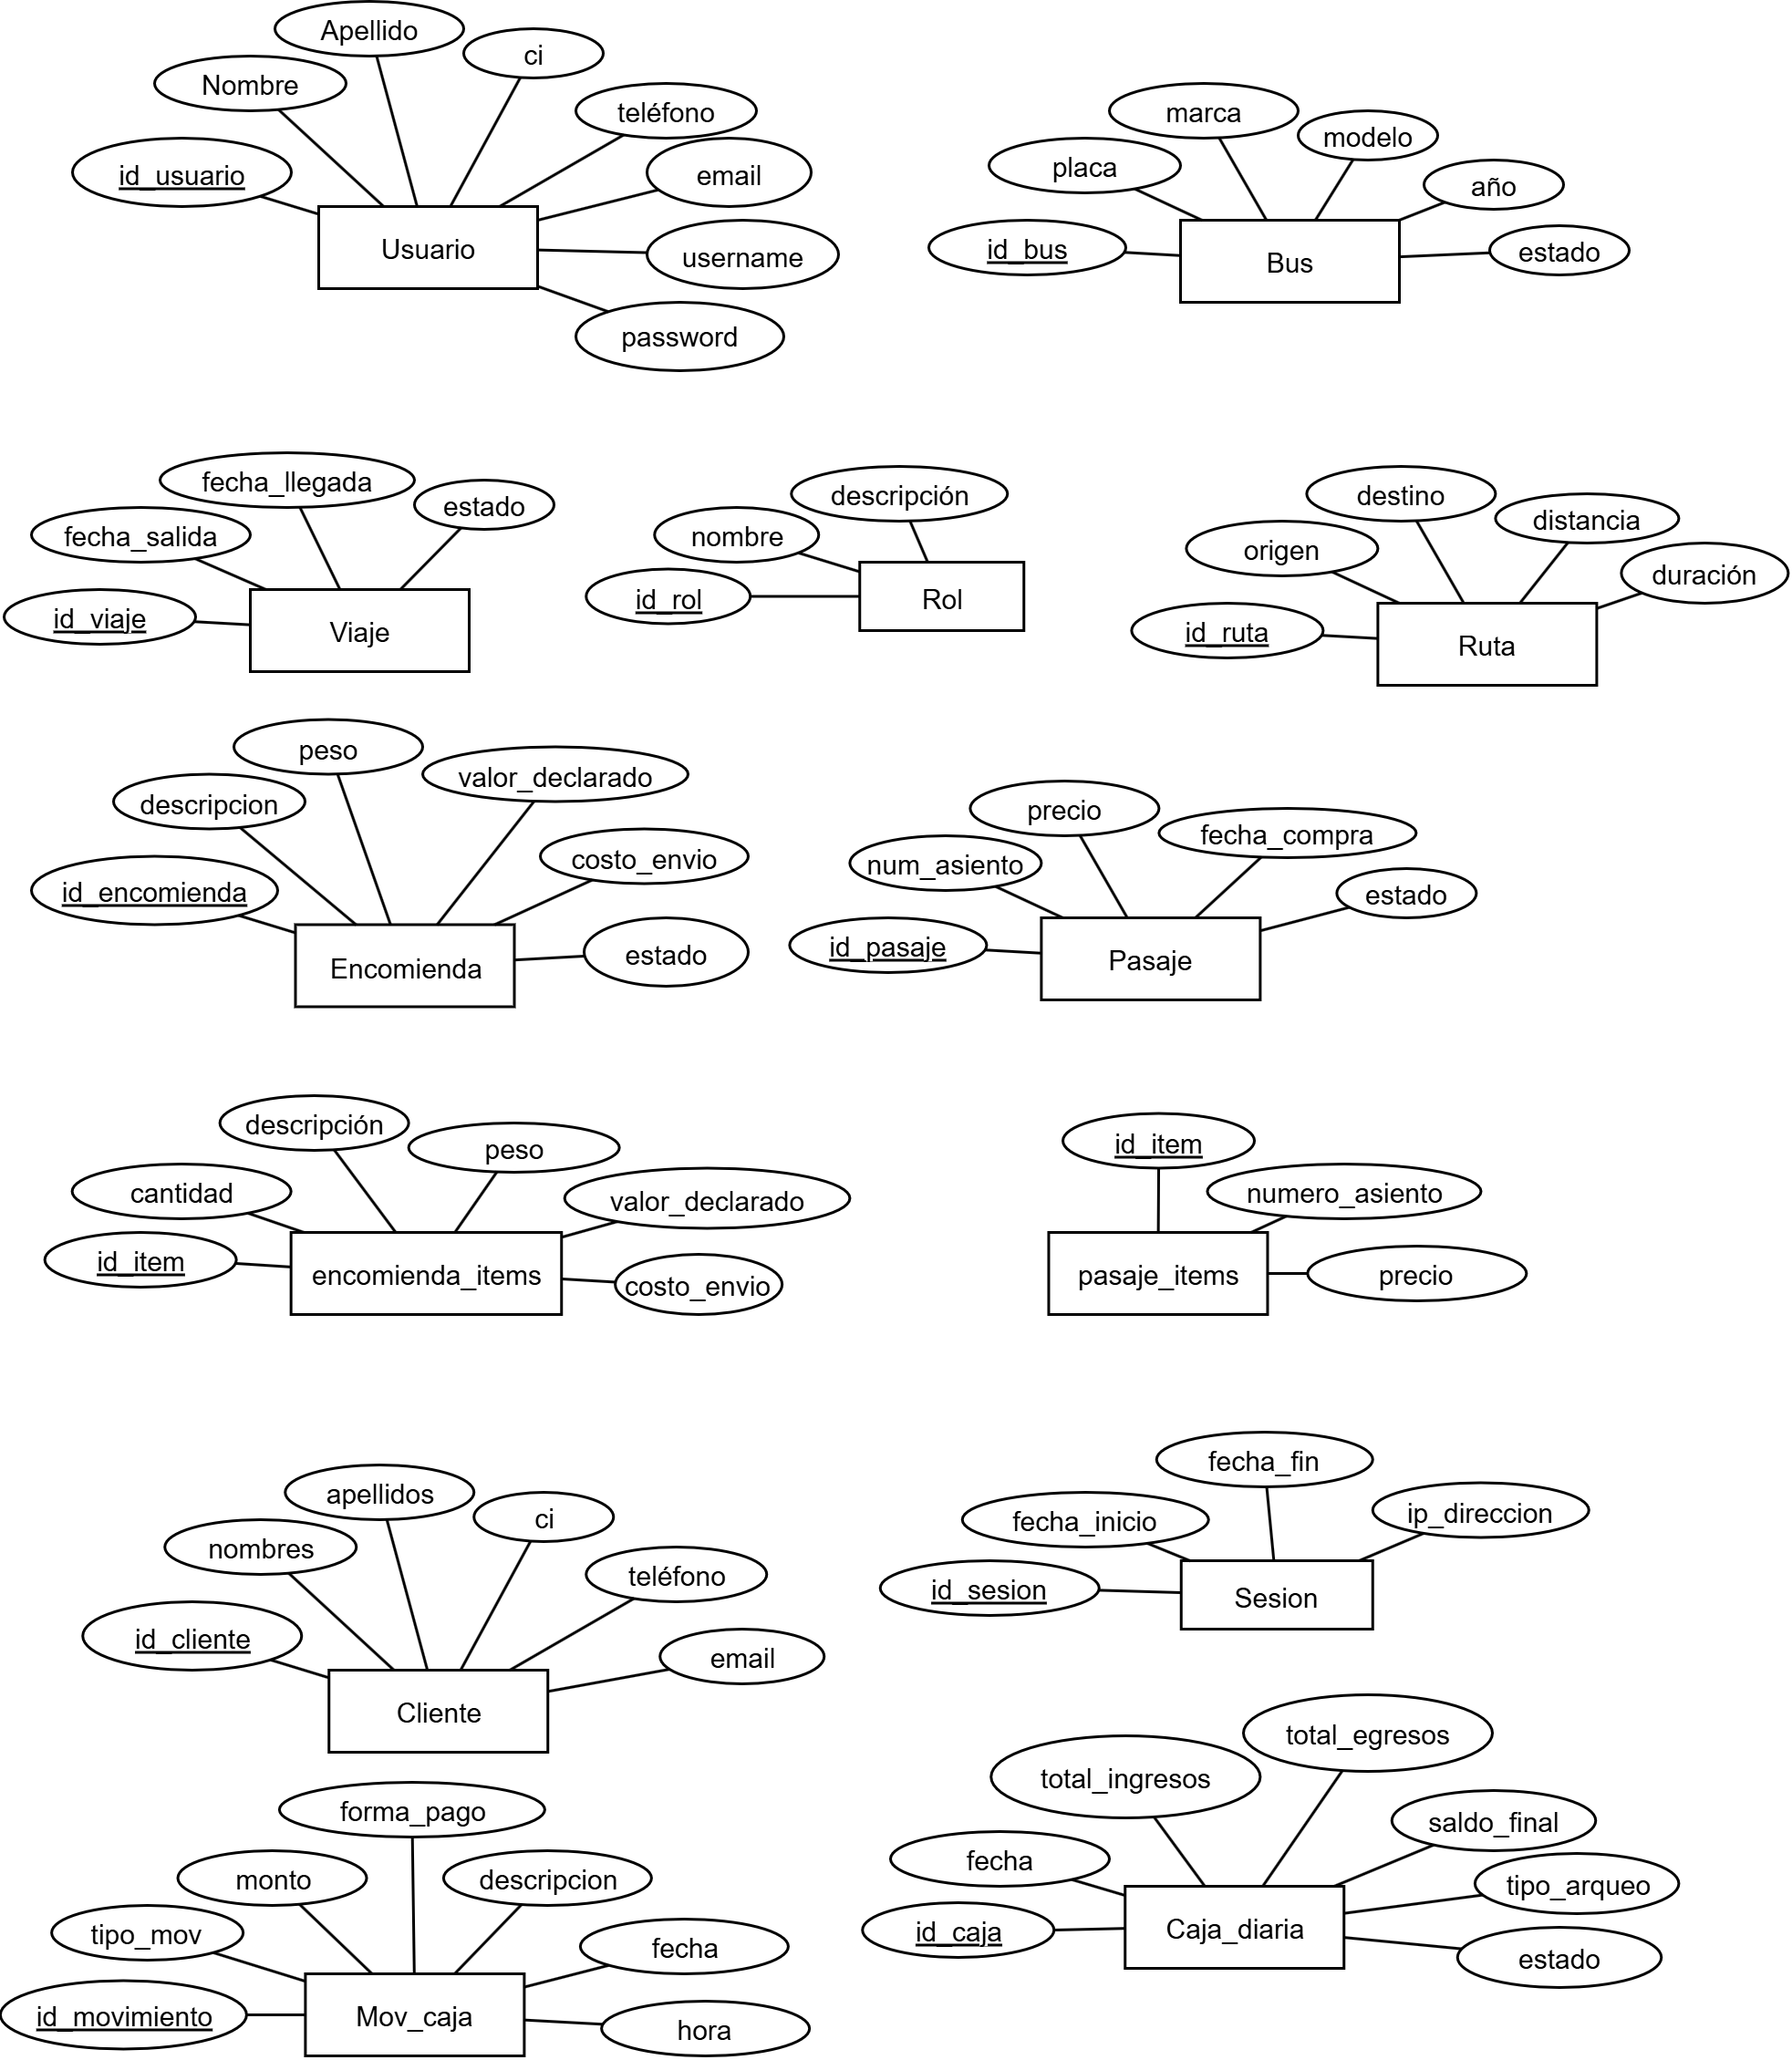
\includegraphics[width=0.9\textwidth]{imagenes/cap_3/MER_ent_atri.png} % Inserta una imagen
		\vspace{0.6cm}
			\caption*{\textup{\textbf{Nota}: El diagrama muestra las entidades del sistema y sus atributos, sin incluir las relaciones entre ellas.}}
		\vspace{-0.6cm}
		\label{fig:ent_atri} % Etiqueta para referencia cruzada
	\end{figure}
	
	La figura \ref{fig:MER_com} representa el modelo entidad-relación, donde se visualizan las conexiones entre las diferentes entidades del sistema. Las líneas de relación muestran cómo las entidades interactúan entre sí, y la cardinalidad especificada en cada relación define las reglas de negocio y las restricciones del sistema.
	
	\begin{figure}[!h] % 'H' del paquete 'float' para mantener posición	
		\caption[Diagrama Entidad-Relación ]
		{\newline Diagrama Entidad-Relación} % Leyenda en la parte superior
		\vspace{0.3cm}
		\centering
		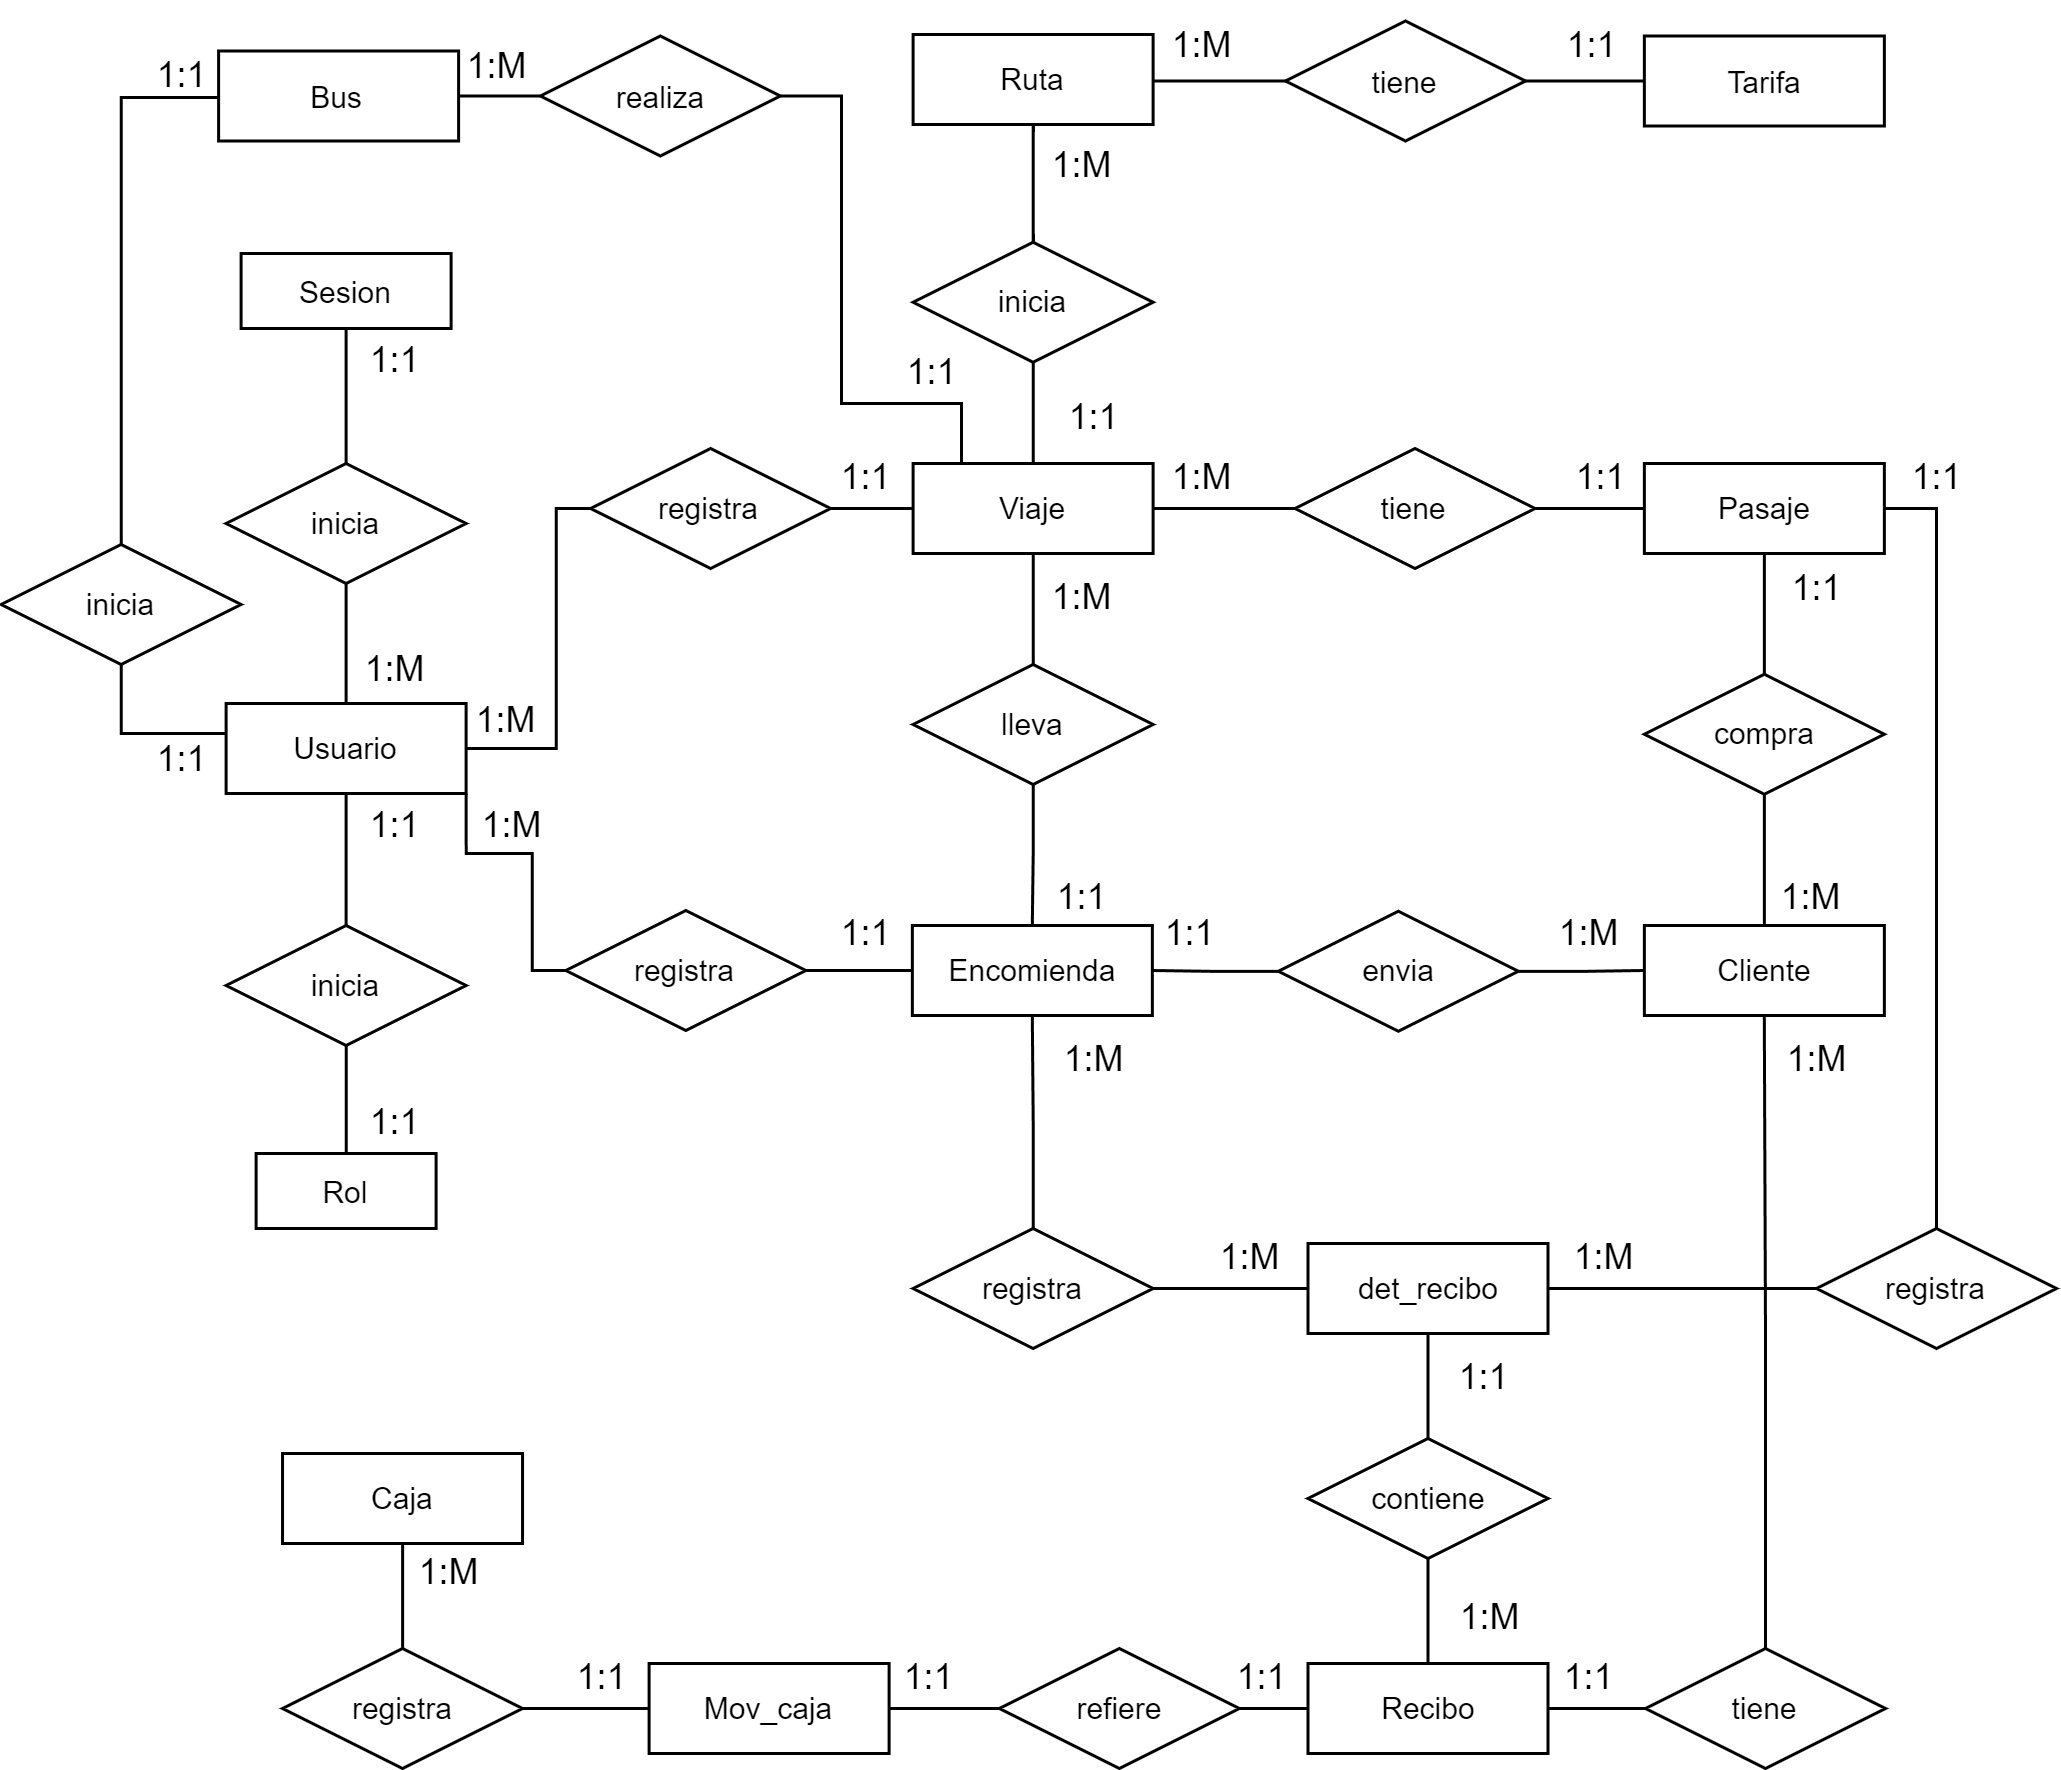
\includegraphics[width=1\textwidth]{imagenes/cap_3/MER_cali.drawio_completo.png} % Inserta una imagen
		\vspace{-0.1cm}
			\caption*{\textup{\textbf{Nota}: El diagrama presenta la estructura lógica de la base de datos del sistema.}}	
		\vspace{-0.6cm}
		\label{fig:MER_com} % Etiqueta para referencia cruzada
	\end{figure}
	
	\subsection{Diagrama relacional}
	En la figura \ref{fig:diag_rela} se presenta el diagrama relacional derivado del modelo entidad-relación mostrado en la figura \ref{fig:ent_atri} y figura \ref{fig:MER_com}.
	
	\vspace{0.3cm} % Agregar 1 cm de espacio entre el párrafo y la figura
	
	\begin{figure}[!h] % 'H' del paquete 'float' para mantener posición	
		\caption[Diagrama Relacional]
		{\newline Diagrama Relacional.} % Leyenda en la parte superior
		\centering
		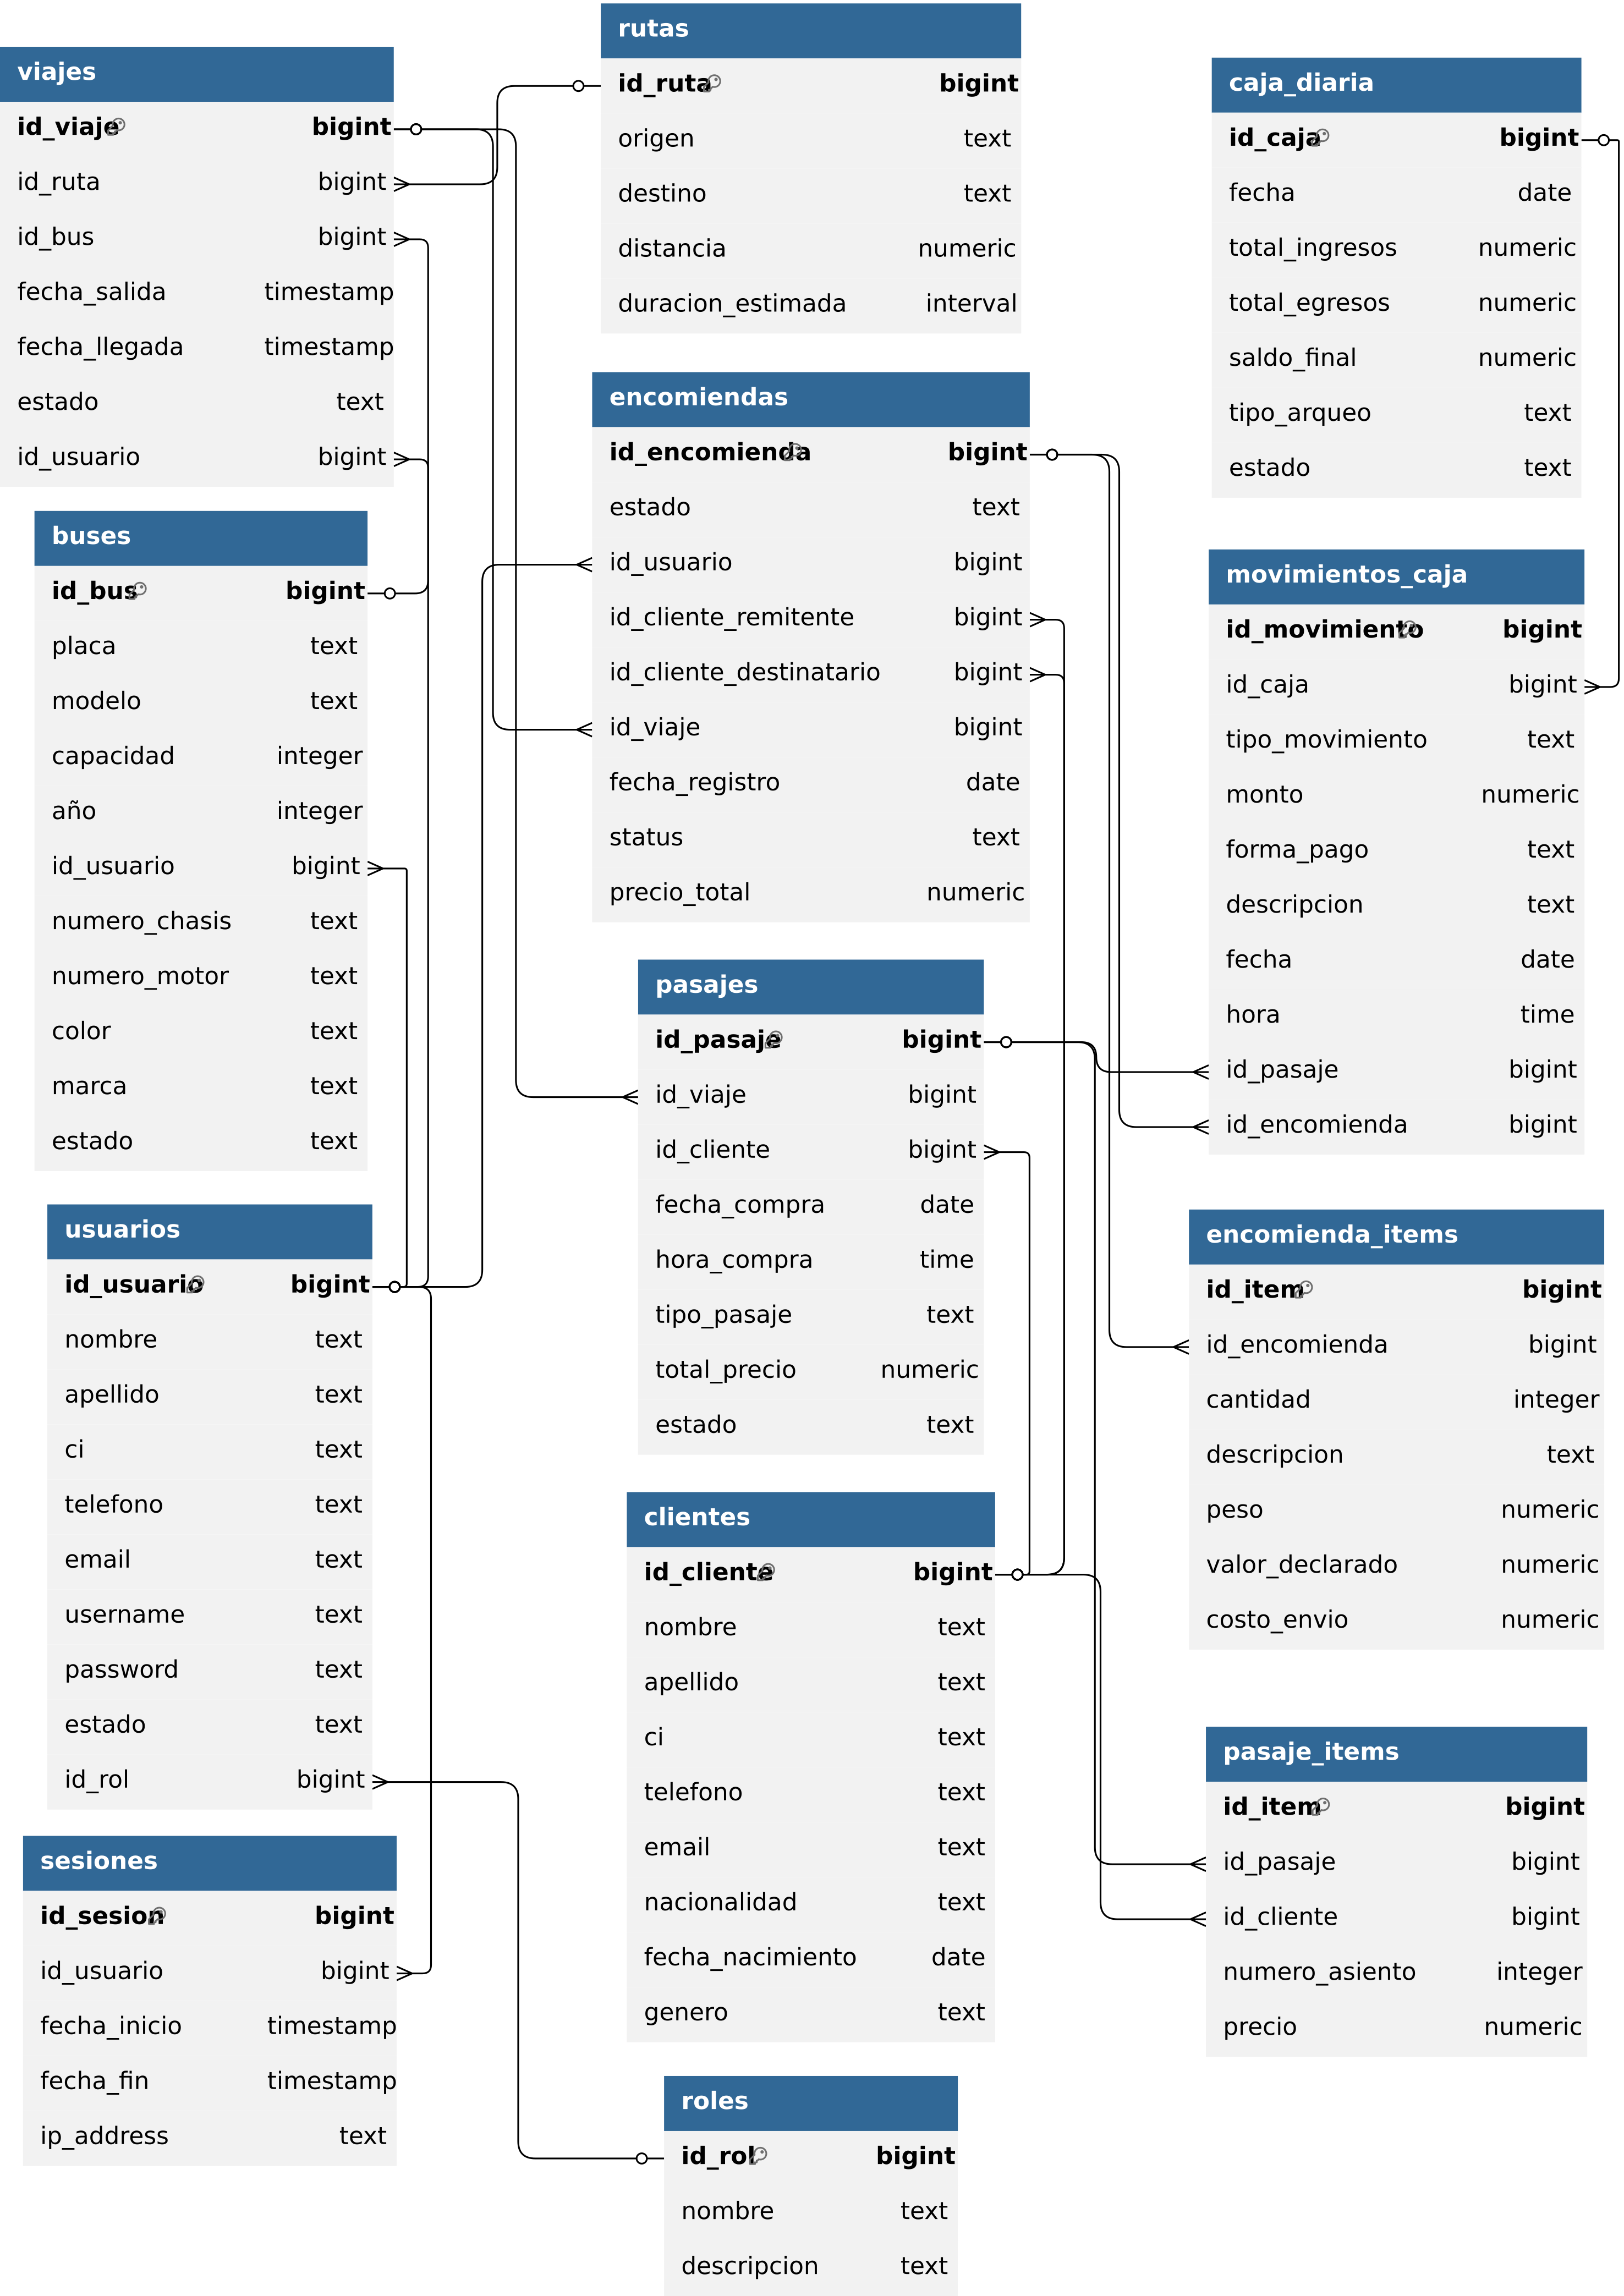
\includegraphics[width=0.8\textwidth]{imagenes/cap_3/modelo_relacional.png} % Inserta una imagen
		
		\begin{flushleft}
			\hspace{1.20cm} \textbf{Nota.} El diagrama representa el modelo relacional derivado del diseño entidad-relacion. % Nota al pie para esta figura
		\end{flushleft}
		\vspace{-16pt}
		\label{fig:diag_rela} % Etiqueta para referencia cruzada
	\end{figure}
	
	Este diagrama refleja la estructura final de la base de datos, organizando las tablas y sus relaciones de acuerdo con las reglas de normalización. A través de este diagrama, se puede visualizar cómo se distribuyen los datos en las distintas tablas, asegurando la eficiencia en el almacenamiento y el manejo adecuado de las relaciones entre las entidades del sistema.
	
	\subsection{Diseño de la interfaz}
	
	El diseño de la interfaz se ha desarrollado para ofrecer una experiencia clara, intuitiva y accesible. Se ha tomado en cuenta la estructura lógica de los procesos del sistema, facilitando que el usuario recorra visualmente los elementos más importantes.
	
	Asimismo, la disposición de botones, formularios, menús y tablas responde a la lógica del escaneo visual en forma de "F", facilitando una rápida adaptación por parte de los usuarios. Este enfoque busca mejorar la eficiencia en la operación diaria, también reducir errores y aumentar la satisfacción del usuario con la herramienta.
	
	\vspace{0.3cm} % Agregar 1 cm de espacio entre el párrafo y la figura
	\begin{figure}[!h] % 'H' del paquete 'float' para mantener posición	
		\caption[Diseño de la página web principal del sistema]
		{\newline Diseño de la página web principal del sistema.} % Leyenda en la parte superior
		\centering
		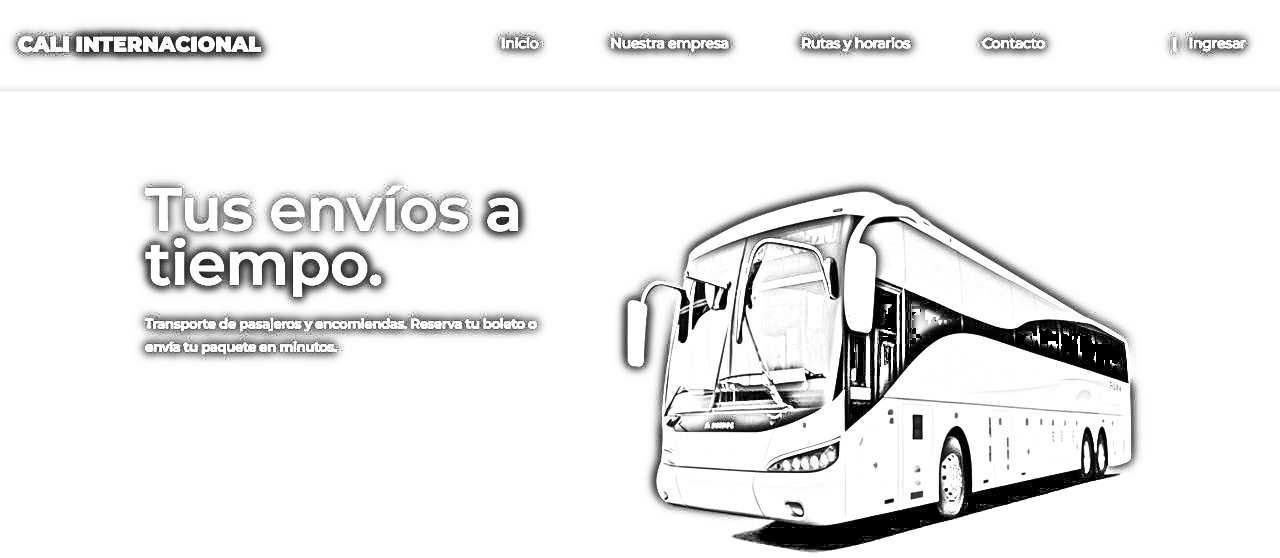
\includegraphics[width=1\textwidth]{imagenes/cap_3/img_diseño/INTER00.png} % Inserta una imagen	
		\begin{flushleft}
			\hspace{1.20cm} \textbf{Nota.} Se presenta una estructura clara con accesos directos accesibles. % Nota al pie para esta figura
		\end{flushleft}
		\vspace{-24pt}
		\label{fig:inter00} % Etiqueta para referencia cruzada
	\end{figure}
	
	La página web principal, como se muestra en la figura \ref{fig:inter00}, presenta una estructura clara y visualmente atractiva para el usuario.
	
	\vspace{-1cm} % Agregar 1 cm de espacio entre el párrafo y la figura
	\begin{figure}[!h] % 'H' del paquete 'float' para mantener posición	
		\caption[Diseño del inicio de sesión]
		{\newline Diseño del inicio de sesión.} % Leyenda en la parte superior
		\centering
		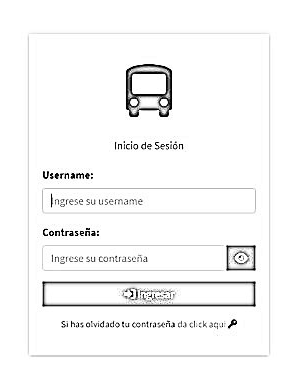
\includegraphics[width=0.33\textwidth]{imagenes/cap_3/img_diseño/INTER01.png} % Inserta una imagen		
		\begin{flushleft}
			\hspace{1.20cm} \textbf{Nota.} Diseño preliminar del inicio de sesión. % Nota al pie para esta figura
		\end{flushleft}
		\vspace{-16pt}
		\label{fig:inter01} % Etiqueta para referencia cruzada
	\end{figure}
	\vspace{0.9cm} % Agregar 1 cm de espacio entre el párrafo y la figura
	
	La figura \ref{fig:inter01}, representa el diseño propuesto para la pantalla de inicio de sesión, enfocado en facilitar el ingreso de usuarios al sistema de forma segura.
	
	% \vspace{0.3cm} % Agregar 1 cm de espacio entre el párrafo y la figura
	\begin{figure}[!h] % 'H' del paquete 'float' para mantener posición	
		\caption[Diseño de la pantalla principal]
		{\newline Diseño de la pantalla principal} % Leyenda en la parte superior
		\centering
		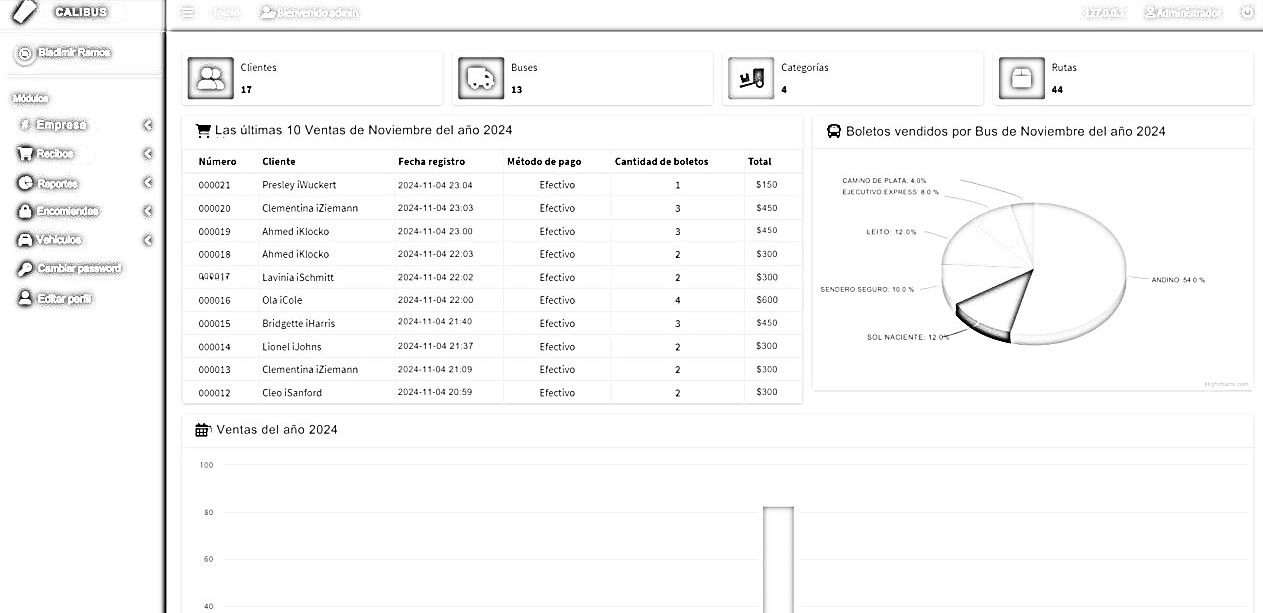
\includegraphics[width=0.8\textwidth]{imagenes/cap_3/img_diseño/INTER02.png} % Inserta una imagen		
		\begin{flushleft}
			\hspace{1.20cm} \textbf{Nota.} Prototipo inicial de la pantalla principal con enfoque en la visualización de reportes. % Nota al pie para esta figura
		\end{flushleft}
		\vspace{-1pt}
		\label{fig:inter02} % Etiqueta para referencia cruzada
	\end{figure}
	\vspace{-0.6cm} % Agregar 1 cm de espacio entre el párrafo y la figura
	
	En la figura \ref{fig:inter02}, se observa el diseño de la vista principal, donde se plantean los elementos visuales para la consulta de reportes de ventas.
	
	
	\vspace{-1cm} % Agregar 1 cm de espacio entre el párrafo y la figura
	\begin{figure}[!h] % 'H' del paquete 'float' para mantener posición	
		\caption[Diseño interfaz Venta de pasajes]
		{\newline Diseño interfaz Venta de pasajes.} % Leyenda en la parte superior
		\centering
		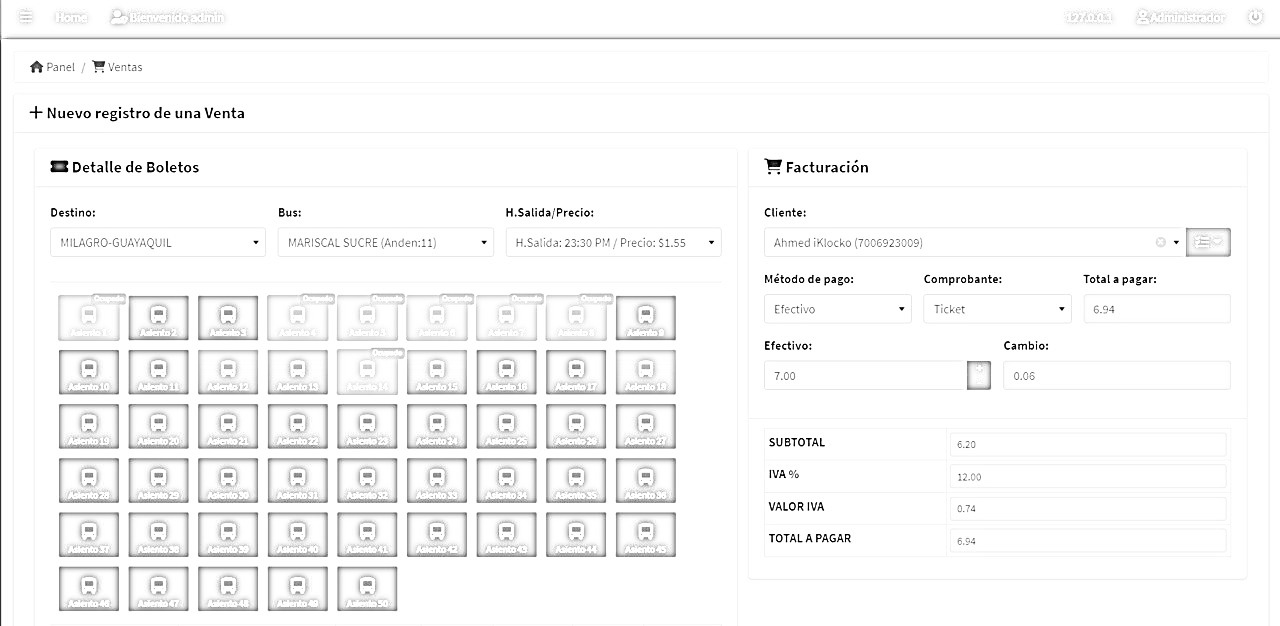
\includegraphics[width=0.80\textwidth]{imagenes/cap_3/img_diseño/INTER03.png} % Inserta una imagen		
		\begin{flushleft}
			\hspace{1.20cm} \textbf{Nota.} Vista conceptual destinada a la venta de pasajes. % Nota al pie para esta figura
		\end{flushleft}
		\vspace{-16pt}
		\label{fig:inter03} % Etiqueta para referencia cruzada
	\end{figure}
	\vspace{0.9cm} % Agregar 1 cm de espacio entre el párrafo y la figura
	
	Como se muestra en la figura \ref{fig:inter03}, el diseño contempla una interfaz para la gestión de pasajes, organizada para agilizar el proceso de venta.
	
	% \vspace{0.3cm} % Agregar 1 cm de espacio entre el párrafo y la figura
	\begin{figure}[!h] % 'H' del paquete 'float' para mantener posición	
		\caption[Diseño interfaz Envío de encomiendas]
		{\newline Diseño interfaz Envío de encomiendas.} % Leyenda en la parte superior
		\centering
		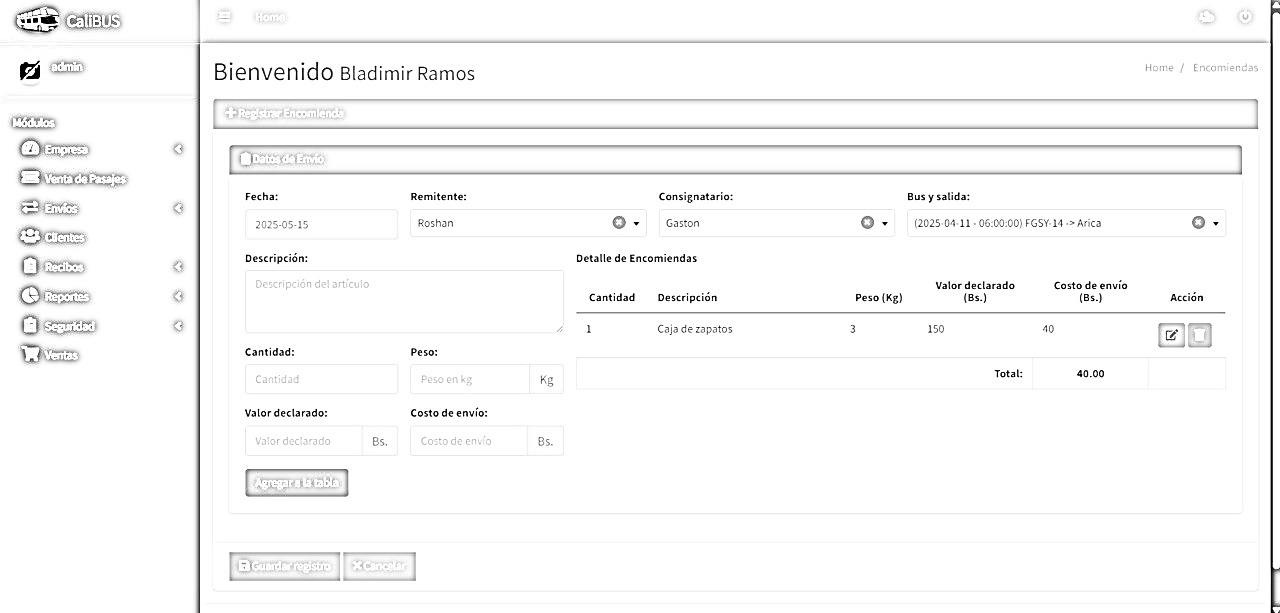
\includegraphics[width=0.80\textwidth]{imagenes/cap_3/img_diseño/INTER04.png} % Inserta una imagen		
		\begin{flushleft}
			\hspace{1.20cm} \textbf{Nota.} Muestra la organización del formulario para gestionar las encomiendas. % Nota al pie para esta figura
		\end{flushleft}
		\vspace{-1pt}
		\label{fig:inter04} % Etiqueta para referencia cruzada
	\end{figure}
	\vspace{-0.6cm} % Agregar 1 cm de espacio entre el párrafo y la figura
	
	La figura \ref{fig:inter04}, corresponde al diseño preliminar de la pantalla destinada al registro y control de envíos de encomiendas.		
		
\section{IMPLEMENTACIÓN Y PRUEBA DE UNIDAD}

	El sistema ha sido desarrollado utilizando el lenguaje de programación Python junto con el framework Django, el cual se seleccionó por su arquitectura robusta basada en el patrón MVT (Model-View-Template). Esta estructura permitió una separación clara entre la lógica del negocio, la gestión de datos y la presentación visual, facilitando tanto el desarrollo modular como el mantenimiento del código. Además, Django proporciona herramientas integradas para la autenticación, la gestión de formularios, la protección contra ataques comunes como CSRF y XSS, y un panel de administración muy útil para la gestión de datos durante el desarrollo.
	
	Durante el proceso de implementación se aplicaron pruebas de unidad a nivel de modelo y vista, con el objetivo de validar que cada componente funcione de forma independiente y según lo esperado. Estas pruebas permitieron detectar y corregir errores en etapas tempranas del desarrollo, mejorando la calidad general del sistema. Se utilizaron las herramientas de prueba integradas en Django, como el módulo TestCase, lo que aseguró una cobertura adecuada del código y una base sólida para futuras extensiones del sistema.
	
	\subsection{Gestión de usuarios}
	La gestión de usuarios se implementa mediante el Programa 3.1, el cual define la vista encargada de controlar el acceso y manejo de las cuentas de usuario dentro del sistema. Esta vista permite realizar operaciones como el inicio de sesión, el cierre de sesión, el registro de nuevos usuarios y la edición de perfiles, todo ello con validaciones que aseguran la integridad de los datos ingresados. El programa se comunica directamente con el modelo de usuarios y aprovecha las herramientas integradas del framework para simplificar el manejo de credenciales y sesiones activas.
	
	Además, el sistema establece distintos niveles de permisos y roles que permiten controlar qué acciones puede realizar cada tipo de usuario. Por ejemplo, ciertos módulos solo están disponibles para administradores, mientras que otros pueden ser accesibles por operadores o personal autorizado. Esto refuerza la seguridad y la organización interna del sistema, permitiendo una administración más eficiente. El diseño modular de este componente facilita futuras ampliaciones, como la integración con sistemas de autenticación externos o la implementación de medidas adicionales como verificación en dos pasos.
		
	\textbf{Programa 3.1}
	
	\textit{Creacion de Usuarios.} % Título y subtítulo alineados
	\vspace{0.3cm} % Espaciado opcional entre el título y el código
	\begin{lstlisting}[lineskip=-1pt]
		class UserCreateView(LoginRequiredMixin, ValidatePermissionRequiredMixin, CreateView):
			model = User
			form_class = UserForm
			template_name = 'user/create.html'
			success_url = reverse_lazy('user:user_list')
			permission_required = 'user.add_user'
			url_redirect = success_url
			
			@method_decorator(csrf_exempt)
			def dispatch(self, request, *args, **kwargs):
				return super().dispatch(request, *args, **kwargs)
			
			def post(self, request, *args, **kwargs):
				data = {}
				try:
					action = request.POST['action']
					if action == 'add':
						form = self.get_form()
						data = form.save()
					else:
						data['error'] = 'No ha ingresado a ninguna opción'
				except Exception as e:
					data['error'] = str(e)
				return JsonResponse(data)
			
			def get_context_data(self, **kwargs):
				context = super().get_context_data(**kwargs)
				context['title'] = 'Creación de un Usuario'
				context['entity'] = 'Usuarios'
				context['list_url'] = self.success_url
				context['action'] = 'add'
				return context
	\end{lstlisting}
	
	\textbf{Nota:} Código que permite la creación de nuevos usuarios al sistema.
	
	\subsection{Gestión de rutas}
	
		El sistema de rutas se implementa a través del Programa 3.2, que establece los modelos necesarios para almacenar la información de rutas correspondientes, y el Programa 3.3, que proporciona las vistas para la gestión de estas entidades. La combinación de estos programas permite una administración eficiente de las rutas y sus programaciones.
		
		\textbf{Programa 3.2}
		
		\textit{Modelo gestión de rutas.} % Título y subtítulo alineados
		\vspace{0.3cm} % Espaciado opcional entre el título y el código
		\begin{lstlisting}[lineskip=-1pt]
			
			class Route(BaseModel):
				origin = models.CharField(
				max_length=100, verbose_name='Origen')
				destination = models.CharField(
				max_length=500, null=True, blank=True, verbose_name='Destino')
				estimated_time = models.CharField(
				max_length=100, null=True, blank=True, verbose_name='Tiempo estimado')
				
				def __str__(self):
					return self.origin
				
				def save(self, force_insert=False, force_update=False, using=None,
					update_fields=None):
					user = get_current_user()
					if user is not None:
						if not self.pk:
							self.user_creation = user
						else:
							self.user_updated = user
					super(Route, self).save()
				
				def toJSON(self):
					item = model_to_dict(self, exclude=['user_creation', 'user_updated'])
					return item
				
				class Meta:
					db_table = 'Rutas'
					verbose_name = 'Ruta'
					verbose_name_plural = 'Rutas'
					ordering = ['id']
		\end{lstlisting}
		
		\textbf{Nota:} Definición del modelo de datos que representa las rutas en el sistema.
		
		\vspace{1cm}
		
		\textbf{Programa 3.3}
		
		\textit{Vista de la gestión de rutas.} % Título y subtítulo alineados
		\vspace{0.3cm} % Espaciado opcional entre el título y el código
		\begin{lstlisting}[lineskip=-1pt]
			
			class RouteListView(LoginRequiredMixin, ValidatePermissionRequiredMixin, ListView):
				model = Route
				template_name = 'route/list.html'
				permission_required = 'calibus.view_route'
				
			@method_decorator(csrf_exempt)
			def dispatch(self, request, *args, **kwargs):
				return super().dispatch(request, *args, **kwargs)
			
			def post(self, request, *args, **kwargs):
				data = {}
				try:
					action = request.POST['action']
					if action == 'searchdata':
						data = []
						for i in Route.objects.all():
						data.append(i.toJSON())
					else:
						data['error'] = 'Ha ocurrido un error'
				except Exception as e:
					data['error'] = str(e)
				return JsonResponse(data, safe=False)
			
			def get_context_data(self, **kwargs):
				context = super().get_context_data(**kwargs)
				context['title'] = 'Listado de rutas'
				context['create_url'] = reverse_lazy('calibus:route_create')
				context['list_url'] = reverse_lazy('calibus:route_list')
				context['entity'] = 'Rutas'
				return context
		\end{lstlisting}
		
		\textbf{Nota:} Código de la interfaz para listar rutas disponibles en el sistema.
	
	\subsection{Gestión de buses}
	
	La gestión de la flota de buses se implementa a través del Programa 3.4, que define el modelo para los buses y su información asociada, y el Programa 3.5, que implementa la vista para la creación de los buses. Estos programas permiten un control completo sobre la flota de buses. Se pueden registrar y editar datos como la placa, capacidad, estado operativo, etc. Además, esta gestión centralizada facilita el seguimiento del mantenimiento, la planificación de horarios y la disponibilidad de unidades, contribuyendo a una operación más eficiente y organizada.
	
	\textbf{Programa 3.4}
	
	\textit{Modelo para la creación de buses.} % Título y subtítulo alineados
	\vspace{0.3cm} % Espaciado opcional entre el título y el código
		\begin{lstlisting}[lineskip=-1pt]
			class Bus(models.Model):
				license_plate = models.CharField(max_length=10, verbose_name="Placa")
				chassis_number = models.CharField(max_length=20, verbose_name="Número de chasis")
				engine_number = models.CharField(max_length=20, verbose_name="Número de motor")
				model = models.CharField(max_length=30, verbose_name="Modelo")
				color = models.CharField(max_length=20, verbose_name="Color")
				brand = models.CharField(max_length=30, verbose_name="Marca")
				capacity = models.PositiveIntegerField(verbose_name="Capacidad")
				year = models.PositiveIntegerField(verbose_name="Año")
				status = models.BooleanField(default=True, verbose_name="Estado")
			
			def __str__(self):
				return self.license_plate
			
			def toJSON(self):
				item = model_to_dict(self)
				return item
			
			class Meta:
				db_table = "Buses"
				verbose_name = "Bus"
				verbose_name_plural = "Buses"
				ordering = ["id"]
		\end{lstlisting}
	
	\textbf{Nota:} Código del modelo de buses de la base de datos.
	
	\textbf{Programa 3.5}
	
	\textit{Vista de la creación de buses.} % Título y subtítulo alineados
	\vspace{0.3cm} % Espaciado opcional entre el título y el código
	\begin{lstlisting}[lineskip=-1pt]
		class BusCreateView(LoginRequiredMixin, ValidatePermissionRequiredMixin, CreateView):
			model = Bus
			form_class = BusForm
			template_name = 'bus/create.html'
			success_url = reverse_lazy('calibus:bus_list')
			permission_required = 'calibus.add_bus'
			url_redirect = success_url
		
		def dispatch(self, request, *args, **kwargs):
			return super().dispatch(request, *args, **kwargs)
		
		def post(self, request, *args, **kwargs):
			data = {}
			try:
				action = request.POST['action']
				if action == 'add':
					form = self.get_form()
					data = form.save()
				else:
					data['error'] = 'No ha ingresado a ninguna opción'
			except Exception as e:
				data['error'] = str(e)
			return JsonResponse(data)
		
		def get_context_data(self, **kwargs):
			context = super().get_context_data(**kwargs)
			context['title'] = 'Creación de un Bus'
			context['entity'] = 'Buses'
			context['list_url'] = self.success_url
			context['action'] = 'add'
			return context
	\end{lstlisting}
	
	\textbf{Nota:} Código de la vista para la creación de buses.
	
	\subsection{Gestión de viajes}
	
	\textbf{Programa 3.6}
	
	\textit{Modelo para la gestión de viajes.} % Título y subtítulo alineados
	\vspace{0.3cm} % Espaciado opcional entre el título y el código
	\begin{lstlisting}[lineskip=-1pt]
		class Travel(models.Model):
			routeID = models.ForeignKey(Route, on_delete=models.CASCADE, verbose_name="Ruta")
			busID = models.ForeignKey(Bus, on_delete=models.CASCADE, verbose_name="Bus")
			departure = models.DateField(default=datetime.now, verbose_name="Fecha de salida")
			departure_time = models.TimeField(default=current_time, verbose_name="Hora de salida")
			arrival = models.DateField(default=datetime.now, verbose_name="Fecha de llegada")
			status = models.CharField(max_length=10,choices=travel_status_choices,default="active",verbose_name="Estado")		
		def __str__(self):
			return f"({self.departure} - {self.departure_time}) {self.busID.license_plate} -> {self.routeID.destination}"		
		def toJSON(self):
			item = model_to_dict(self)
			item["route"] = self.routeID.toJSON()
			return item		
		class Meta:
			db_table = "Viajes"
			verbose_name = "Viaje"
			verbose_name_plural = "Viajes"
			ordering = ["id"]
	\end{lstlisting}
	
	\textbf{Nota:} Modelo para pa gestión de viajes.
	
	La gestión de viajes se implementa mediante el Programa 3.6, que define el modelo con la información relevante de cada viaje, como fecha, hora, ruta y bus asignado. El Programa 3.7 complementa esta funcionalidad al presentar una vista tipo lista donde se muestran todos los viajes registrados. Esta vista permite filtrar, editar o eliminar viajes de forma rápida y ordenada.
	
	\textbf{Programa 3.7}
	
	\textit{Vista para el listado de viajes.} % Título y subtítulo alineados
	\vspace{0.3cm} % Espaciado opcional entre el título y el código
	\begin{lstlisting}[lineskip=-1pt]
		class TravelListView(LoginRequiredMixin, ValidatePermissionRequiredMixin, ListView):
			model = Travel
			template_name = 'travel/list.html'
			permission_required = 'calibus.view_travel'
		
		@method_decorator(csrf_exempt)
		def dispatch(self, request, *args, **kwargs):
			return super().dispatch(request, *args, **kwargs)
		
		def post(self, request, *args, **kwargs):
			data = {}
			try:
				action = request.POST['action']
				if action == 'searchdata':
					data = []
					for i in Travel.objects.all():
						data.append(i.toJSON())
				else:
				data['error'] = 'Ha ocurrido un error'
			except Exception as e:
				data['error'] = str(e)
			return JsonResponse(data, safe=False)
		
		def get_context_data(self, **kwargs):
			context = super().get_context_data(**kwargs)
			context['title'] = 'Listado de Viajes'
			context['create_url'] = reverse_lazy('calibus:travel_create')
			context['list_url'] = reverse_lazy('calibus:travel_list')
			context['entity'] = 'Viajes'
			context['parent'] = 'empresa'
			context['segment'] = 'viaje'
			return context
	\end{lstlisting}
	
	\textbf{Nota:} Vista tipo lista que permita visualizar, filtrar y administrar los viajes registrados en el sistema.
	
	\subsection{Venta y reserva de pasajes}
		
		El sistema de venta y reservas se implementa mediante el Programa 3.8, que define el modelo de clientes para los datos de la venta y/o reserva de pasajes, el Programa 3.9, muestra el modelo para la gestión de viajes. Estos programas trabajan en conjunto para garantizar la integridad de las transacciones y prevenir conflictos en ventas y/o reservas simultáneas.
		
		\textbf{Programa 3.8}
		
		\textit{Modelo para la gestión de pasajes.} % Título y subtítulo alineados
		\vspace{0.3cm} % Espaciado opcional entre el título y el código
		\begin{lstlisting}[lineskip=-1pt]
			
			class Ticket(models.Model):
				clientID = models.ForeignKey(Client, on_delete=models.CASCADE)
				travelID = models.ForeignKey(Travel, on_delete=models.CASCADE)
				purchase_date = models.DateField(default=datetime.now, verbose_name="Fecha de compra")
				purchase_time = models.TimeField(default=current_time, verbose_name="Hora de compra")
				ticket_type = models.CharField(max_length=20,choices=ticket_type_choices,default="libre",verbose_name="Tipo de pasaje",)
				total_price = models.DecimalField(default=0.00, max_digits=9, decimal_places=2,verbose_name="Precio total")
				status = models.BooleanField(default=True, verbose_name="Estado")			
				def __str__(self):
					return f"Ticket de {self.clientID.names} para el viaje {self.travelID.id}"
			
				def toJSON(self):
					data = model_to_dict(self)
					data["clientID"] = (f"{self.clientID.names} {self.clientID.surnames}"  # Combina nombres y apellidos)
					data["travelID"] = (f"{self.travelID.routeID.origin} -> {self.travelID.routeID.destination} ({self.travelID.departure}{self.travelID.departure_time})")
					return data
				class Meta:
					db_table = "Pasajes"
					verbose_name = "Pasaje"
					verbose_name_plural = "Pasajes"
					ordering = ["id"]			
		\end{lstlisting}
		
		\textbf{Nota:} Modelo que gestiona la venta y reserva de pasajes, incluyendo datos del pasajero, asiento, viaje.
		
		\textbf{Programa 3.9}
		
		\textit{Vista para el registro de pasajes.} % Título y subtítulo alineados
		\vspace{0.3cm} % Espaciado opcional entre el título y el código
		\begin{lstlisting}[lineskip=-1pt]
			class TicketCreateView(LoginRequiredMixin, ValidatePermissionRequiredMixin, CreateView):
				model = Ticket
				form_class = TicketForm
				template_name = "ticket/create.html"
				success_url = reverse_lazy("index")
				permission_required = "calibus.add_ticket"
				url_redirect = success_url			
			def dispatch(self, request, *args, **kwargs):
				return super().dispatch(request, *args, **kwargs)			
			def post(self, request, *args, **kwargs):
				data = {}
				try:
					action = request.POST["action"]
					if action == "add":
						form = self.get_form()
						data = form.save()
					else:
						data["error"] = "No ha ingresado a ninguna opción"
				except Exception as e:
					data["error"] = str(e)
				return JsonResponse(data)			
			def get_context_data(self, **kwargs):
				context = super().get_context_data(**kwargs)
				context["title"] = "Registro de Pasajes"
				context["entity"] = "Pasajes"
				context["list_url"] = self.success_url
				context["action"] = "add"
				travel_id = self.request.GET.get("travel")
				if travel_id:
					try:
						travel = Travel.objects.get(pk=travel_id)
						bus = travel.busID
						context["travel"] = travel
						context["bus"] = bus
						context["total_seats"] = bus.capacity
						print("DEBUG bus.capacity:", bus.capacity)  
					except Travel.DoesNotExist:
						context["travel"] = None
						context["bus"] = None
						context["total_seats"] = 0
				else:
					context["travel"] = None
					context["bus"] = None
					context["total_seats"] = 0
				return context
		\end{lstlisting}
		
		\textbf{Nota:} Vista para registrar ventas o reservas de pasajes, con validaciones para evitar duplicidades y conflictos de asignación.
			
	\subsection{Registro de encomiendas}
	
		El sistema de encomiendas se implementa mediante el Programa 3.10, que define el modelo para el registro y seguimiento de encomiendas, y el Programa 3.11, que proporciona la vista para la creación y gestión de encomiendas. Estos programas permiten un seguimiento detallado de cada encomienda en el sistema.
		
		\textbf{Programa 3.10}
		
		\textit{Modelo para el registro de encomiendas.} % Título y subtítulo alineados
		\vspace{0.3cm} % Espaciado opcional entre el título y el código
		\begin{lstlisting}[lineskip=-1pt]
			class Parcel(models.Model):
				senderID = models.ForeignKey(Client,on_delete=models.CASCADE,related_name="sent_parcels")
				receiverID = models.ForeignKey(Client, on_delete=models.CASCADE,related_name="received_parcels")
				travelID = models.ForeignKey(Travel, on_delete=models.CASCADE)
				date_joined = models.DateField(default=datetime.now, verbose_name="Fecha de registro")
				status = models.CharField(max_length=30,choices=parcel_choices,default="pending",verbose_name="Estado",blank=True,)
				total = models.DecimalField(default=0.00,max_digits=10,decimal_places=2,verbose_name="Total Precio de Envío",)
			
				def __str__(self):
					return self.senderID.names
						
				def toJSON(self):
					data = model_to_dict(self)
					data["senderID"] = (f"{self.senderID.names} {self.senderID.surnames}"  # Combina nombres y apellidos)
					data["receiverID"] = f"{self.receiverID.names} {self.receiverID.surnames}"
					data["travelID"] = (f"{self.travelID.routeID.origin} -> {self.travelID.routeID.destination} ({self.travelID.departure} {self.travelID.departure_time})")
					return data
			
				class Meta:
					db_table = "Encomiendas"
					verbose_name = "Encomienda"
					verbose_name_plural = "Encomiendas"
					ordering = ["id"]
		\end{lstlisting}
		
		\textbf{Nota:} Modelo que estructura los datos de las encomiendas, incluyendo remitente, consignatario y datos del envío.
		
		\textbf{Programa 3.11}
		
		\textit{Vista para la creación de encomiendas} % Título y subtítulo alineados
		\vspace{0.3cm} % Espaciado opcional entre el título y el código
		\begin{lstlisting}[lineskip=-1pt]
		class ParcelCreateView(LoginRequiredMixin, ValidatePermissionRequiredMixin, CreateView):
			model = Parcel
			form_class = ParcelForm
			template_name = 'parcel/create.html'
			success_url = reverse_lazy('index')
			permission_required = 'calibus.add_parcel'
			url_redirect = success_url
			
			def dispatch(self, request, *args, **kwargs):
			return super().dispatch(request, *args, **kwargs)
			
			def post(self, request, *args, **kwargs):
				data = {}
				try:
					action = request.POST['action']
					if action == 'add':
						form = self.get_form()
						data = form.save()
					else:
						data['error'] = 'No ha ingresado a ninguna opción'
				except Exception as e:
					data['error'] = str(e)
				return JsonResponse(data)
			
			def get_context_data(self, **kwargs):
				context = super().get_context_data(**kwargs)
				context['title'] = 'Creación una Encomienda'
				context['entity'] = 'Encomiendas'
				context['list_url'] = self.success_url
				context['action'] = 'add'
				return context
		\end{lstlisting}
		
		\textbf{Nota:} Vista que permite registrar, actualizar y gestionar el seguimiento de encomiendas dentro del sistema.
	
	\subsection{Gestión de clientes}
	
		La gestión de clientes se implementa mediante el Programa 3.12, que define el modelo encargado de almacenar la información personal y de contacto de los clientes.  Complementando esta funcionalidad, el Programa 3.13 proporciona la vista para el registro y edición de clientes, permitiendo una administración eficiente y centralizada de los datos esenciales para los procesos de envíos de encomiendas.
	
	\textbf{Programa 3.12}
	
	\textit{Modelo para la gestión de clientes.} % Título y subtítulo alineados
	\vspace{0.3cm} % Espaciado opcional entre el título y el código
	\begin{lstlisting}[lineskip=-1pt]
		class Client(models.Model):
			names = models.CharField(max_length=150, verbose_name="Nombres")
			surnames = models.CharField(max_length=150, verbose_name="Apellidos")
			ci = models.CharField(
			max_length=10, unique=True, verbose_name="Cédula de Identidad")
			nationality = models.CharField(max_length=20, default="Desconocido",verbose_name="Nacionalidad")
			date_of_birth = models.DateField(default=datetime.now, verbose_name="Fecha de nacimiento")
			phone = models.CharField(max_length=10, verbose_name="Teléfono")
			email = models.CharField(max_length=100, verbose_name="Correo electrónico")
			gender = models.CharField(max_length=10, choices=gender_choices, default="male",verbose_name="Sexo")
		
			def __str__(self):
				return self.names
			
			def toJSON(self):
				item = model_to_dict(self)
				item["gender"] = {"id": self.gender, "name": self.get_gender_display()}
				return item
		
			class Meta:
				db_table = "Clientes"
				verbose_name = "Cliente"
				verbose_name_plural = "Clientes"
				ordering = ["id"]
	\end{lstlisting}
	
	\textbf{Nota:} Modelo que almacena los datos personales de los clientes.
	
	\textbf{Programa 3.13}
	
	\textit{Vista para el registro de clientes.} % Título y subtítulo alineados
	\vspace{0.3cm} % Espaciado opcional entre el título y el código
	\begin{lstlisting}[lineskip=-1pt]
		class ClientCreateView(LoginRequiredMixin, ValidatePermissionRequiredMixin, CreateView):
			model = Client
			form_class = ClientForm
			template_name = 'client/create.html'
			success_url = reverse_lazy('calibus:client_list')
			permission_required = 'calibus.add_client'
			url_redirect = success_url
		
			def dispatch(self, request, *args, **kwargs):
				return super().dispatch(request, *args, **kwargs)
		
			def post(self, request, *args, **kwargs):
				data = {}
				try:
					action = request.POST['action']
					if action == 'add':
						form = self.get_form()
						data = form.save()
					else:
						data['error'] = 'No ha ingresado a ninguna opción'
				except Exception as e:
					data['error'] = str(e)
				return JsonResponse(data)
			
			def get_context_data(self, **kwargs):
				context = super().get_context_data(**kwargs)
				context['title'] = 'Creación un Cliente'
				context['entity'] = 'Clientes'
				context['list_url'] = self.success_url
				context['action'] = 'add'
				return context
	\end{lstlisting}
	
	\textbf{Nota:} Vista destinada al registro y edición de cleintes, facilitando su administración dentro del sistema.	
	
\section{PRUEBA DE SISTEMA}
	\subsection{Pruebas unitarias}
	
	En el marco del desarrollo del proyecto, enfocado en la gestión de usuarios, la venta de pasajes y el envío de encomiendas, las pruebas unitarias desempeñan un papel fundamental para garantizar la calidad y fiabilidad del sistema. Implementadas mediante la herramienta unittest de Python, estas pruebas aseguran que cada componente funcione correctamente y cumpla con los requisitos establecidos.
	
	Las pruebas se aplicaron principalmente a los modelos y vistas, evaluando el comportamiento de funciones clave como la autenticación de usuarios, la venta o reserva de pasajes y el registro de encomiendas. Este proceso no solo valida que los datos se almacenen y gestionen adecuadamente, sino que también fortalece la estabilidad del sistema ante posibles modificaciones futuras.
	
	El Programa 3.14 contiene las pruebas relacionadas con la gestión de usuarios. Este archivo incluye los siguientes casos de prueba:
	
	\textbf{Programa 3.14}
	
	\textit{Pruebas de Gestión de Usuarios.} % Título y subtítulo alineados
	\vspace{0.3cm} % Espaciado opcional entre el título y el código
	\begin{lstlisting}[lineskip=-1pt]
		class PruebasGestionUsuario(unittest.TestCase):
		def setUp(self):
			# Inicializa el servicio de usuario que vamos a probar
			self.servicio_usuario = ServicioUsuario()
		
		# Prueba 1: Verificar que un usuario se puede registrar correctamente
		def test_registro_usuario_exitoso(self):
		# Datos de prueba para el registro
		datos_usuario = {
			"email": "bladi.ram@gmail.com",
			"password": "Contraseña123",
			"nombre": "Bladimir",
			"apellido": "Ramos",
			"telefono": "1234567"
		}
		# Intenta registrar al usuario
		resultado = self.servicio_usuario.registrar_usuario(datos_usuario)
		
		# Verifica que el registro fue exitoso
		self.assertTrue(resultado.exito)  
		self.assertIsNotNone(resultado.id_usuario)
		
		# Prueba 2: Verificar que un usuario puede iniciar sesión correctamente
		def test_login_usuario_exitoso(self):
		# Credenciales de prueba
		credenciales = {
			"email": "bladi.ram@gmail.com",
			"password": "Contraseña123"
		}
		# Intenta iniciar sesión
		resultado = self.servicio_usuario.iniciar_sesion(credenciales)
		
		# Verifica que el login fue exitoso
		self.assertTrue(resultado.exito)  
		self.assertIsNotNone(resultado.token_sesion)  
		
		# Prueba 3: Verificar que el sistema rechaza credenciales incorrectas
		def test_credenciales_invalidas(self):
		# Credenciales incorrectas de prueba
		credenciales = {
			"email": "prueba@gmail.com",
			"password": "ContraseñaIncorrecta"
		}
		# Intenta iniciar sesión con credenciales incorrectas
		resultado = self.servicio_usuario.iniciar_sesion(credenciales)
		
		# Verifica que el login falló como se esperaba
		self.assertFalse(resultado.exito)  
		self.assertEqual(resultado.mensaje_error, "Credenciales inválidas")  
	\end{lstlisting}
	
	\textbf{Nota:} Pruebas unitarias para validar el funcionamiento del registro de usuarios.
	
	El Programa 3.15 evalúa funcionalidades asociadas a la venta y reserva de pasajes. 		
	
	\textbf{Programa 3.15}
	
	\textit{Pruebas de venta y reserva de pasajes.} % Título y subtítulo alineados
	\vspace{0.3cm} % Espaciado opcional entre el título y el código
	\begin{lstlisting}[lineskip=-1pt]
		class PruebasReservaPasajes(unittest.TestCase):
		
		def setUp(self):
		self.servicio_reservas = ServicioReservas()
		self.id_usuario = "12"
		
		def test_verificar_disponibilidad_pasajes(self):
		parametros_busqueda = {
			"origen": "La Paz",
			"destino": "Arica",
			"fecha": datetime(2024, 12, 1),
			"pasajes": 2
		}
		resultado = self.servicio_reservas.verificar_disponibilidad(parametros_busqueda)
		self.assertTrue(resultado.exito)
		self.assertGreater(len(resultado.pasajes_disponibles), 0)
		
		def test_reserva_pasaje_exitosa(self):
		datos_reserva = {
			"id_usuario": self.id_usuario,
			"id_viaje": "13",
			"pasajeros": [
			{"name": "Juan Pérez", "asiento": "12A"},
			{"name": "María Pérez", "asiento": "12B"}
			],
			"info_pago": {
				"method": "Efectivo",
				"mount": 300.00
			}
		}
		resultado = self.servicio_reservas.reservar_pasaje(datos_reserva)
		self.assertTrue(resultado.exito)
		self.assertIsNotNone(resultado.id_reserva)
		self.assertIsNotNone(resultado.codigo_confirmacion)
		
		def test_cancelacion_reserva(self):
		id_reserva = "23"
		resultado = self.servicio_reservas.cancelar_reserva(id_reserva, self.id_usuario)
		self.assertTrue(resultado.exito)
		self.assertIsNotNone(resultado.monto_reembolso)	
	\end{lstlisting}
	
	\textbf{Nota:} Pruebas que verifican el proceso de venta y reserva de pasajes, incluyendo validaciones de disponibilidad y asignación de asientos.
	
	\vspace{2cm}
	
	El Programa 3.16 está dedicado a las pruebas del módulo de envío de encomiendas.
	
	\textbf{Programa 3.16}
	
	\textit{Pruebas de Gestión de Encomiendas.} % Título y subtítulo alineados
	\vspace{0.3cm} % Espaciado opcional entre el título y el código
	\begin{lstlisting}[lineskip=-1pt]
		
		class PruebaModeloParcel(TestCase):
		
			def setUp(self):
			
				self.remitente = Client.objects.create(
				names="Carlos", surnames="Ramírez", email="carlos@example.com"
				)
				self.destinatario = Client.objects.create(
				names="Lucía", surnames="Gómez", email="lucia@example.com"
				)
				self.viaje = Travel.objects.create(
				routeID_id=1,
				departure=datetime(2024, 12, 10),
				departure_time="10:00"
				)
				
				self.encomienda = Parcel.objects.create(
				senderID=self.remitente,
				receiverID=self.destinatario,
				travelID=self.viaje,
				status="pending",
				total=120.50
				)
			
			def test_creacion_encomienda(self):
			
				"""Verifica que se crea correctamente una encomienda"""
				self.assertEqual(self.encomienda.senderID.names, "Carlos")
				self.assertEqual(self.encomienda.receiverID.names, "Lucía")
				self.assertEqual(str(self.encomienda), "Carlos")
				self.assertEqual(self.encomienda.status, "pending")
				self.assertGreater(self.encomienda.total, 0)
			
			def test_representacion_json(self):
			
				"""Verifica el método toJSON() de encomienda"""
				json_data = self.encomienda.toJSON()
				self.assertIn("senderID", json_data)
				self.assertIn("receiverID", json_data)
				self.assertIn("travelID", json_data)
				self.assertEqual(json_data["senderID"], "Carlos Ramírez")
				
	\end{lstlisting}
	
	\textbf{Nota:} Pruebas unitarias orientadas a verificar el registro correcto de las encomiendas.
		
	\subsection{Resultados de las pruebas}
	
	En la figura \ref{fig:prue_uni}, se observa los resultados de las tres pruebas realizadas.
	
	\vspace{0.2cm} % Agregar 1 cm de espacio entre el párrafo y la figura
	
	\begin{figure}[!h] % 'H' del paquete 'float' para mantener posición	
		\caption[Pruebas Unitarias]
		{\newline Pruebas Unitarias.} % Leyenda en la parte superior
		\centering
		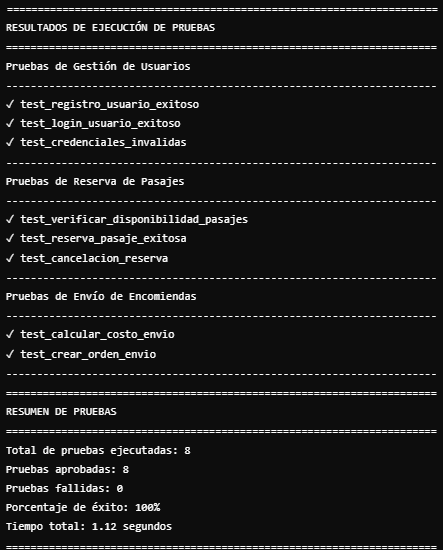
\includegraphics[width=0.65\textwidth]{imagenes/cap_3/pruebas_unitarias.png} % Inserta una imagen
		\begin{flushleft}
			\hspace{1.20cm} \textbf{Nota.} Resultados generados tras la ejecución de las pruebas unitarias. % Nota al pie para esta figura
		\end{flushleft}
		%\vspace{-16pt}
		\label{fig:prue_uni} % Etiqueta para referencia cruzada
	\end{figure}
	\vspace{-20pt} % Agregar 1 cm de espacio entre el párrafo y la figura
	
	Estas pruebas no solo facilitaron la detección de errores en etapas tempranas del desarrollo, sino que también incrementan la confianza en el sistema, garantizando que cada módulo funcione de manera independiente y que los cambios no introduzcan fallos. Además, al integrarlas en un flujo de trabajo continuo, permiten un desarrollo seguro, reduciendo los tiempos de corrección.
	
 \section{OPERACIÓN Y MANTENIMIENTO}
 
 	La fase de Operación y Mantenimiento corresponde a la etapa final del modelo en cascada, en la cual el sistema entra en funcionamiento real y es utilizado por los usuarios finales, durante esta fase, se supervisa el comportamiento del sistema para garantizar su correcto desempeño en un entorno de producción. Además, se da seguimiento a posibles incidencias, errores o mejoras solicitadas por los usuarios, lo que permite realizar ajustes que aseguren la estabilidad y continuidad operativa del sistema.
 	
 	En esta etapa, se han documentado las interfaces implementadas mediante capturas de pantalla representativas, como se muestra en las figuras correspondientes, la recopilación de estas vistas proporciona evidencia visual del sistema en operación, permitiendo evaluar su funcionalidad desde el punto de vista práctico, así como servir de base para futuras tareas de mantenimiento y mejora continua.
 
 % \vspace{0.3cm} % Agregar 1 cm de espacio entre el párrafo y la figura
 \begin{figure}[!h] % 'H' del paquete 'float' para mantener posición	
 	\caption[Página web - Cali Internacional]
 	{\newline Página web - Cali Internacional.} % Leyenda en la parte superior
 	\centering
 	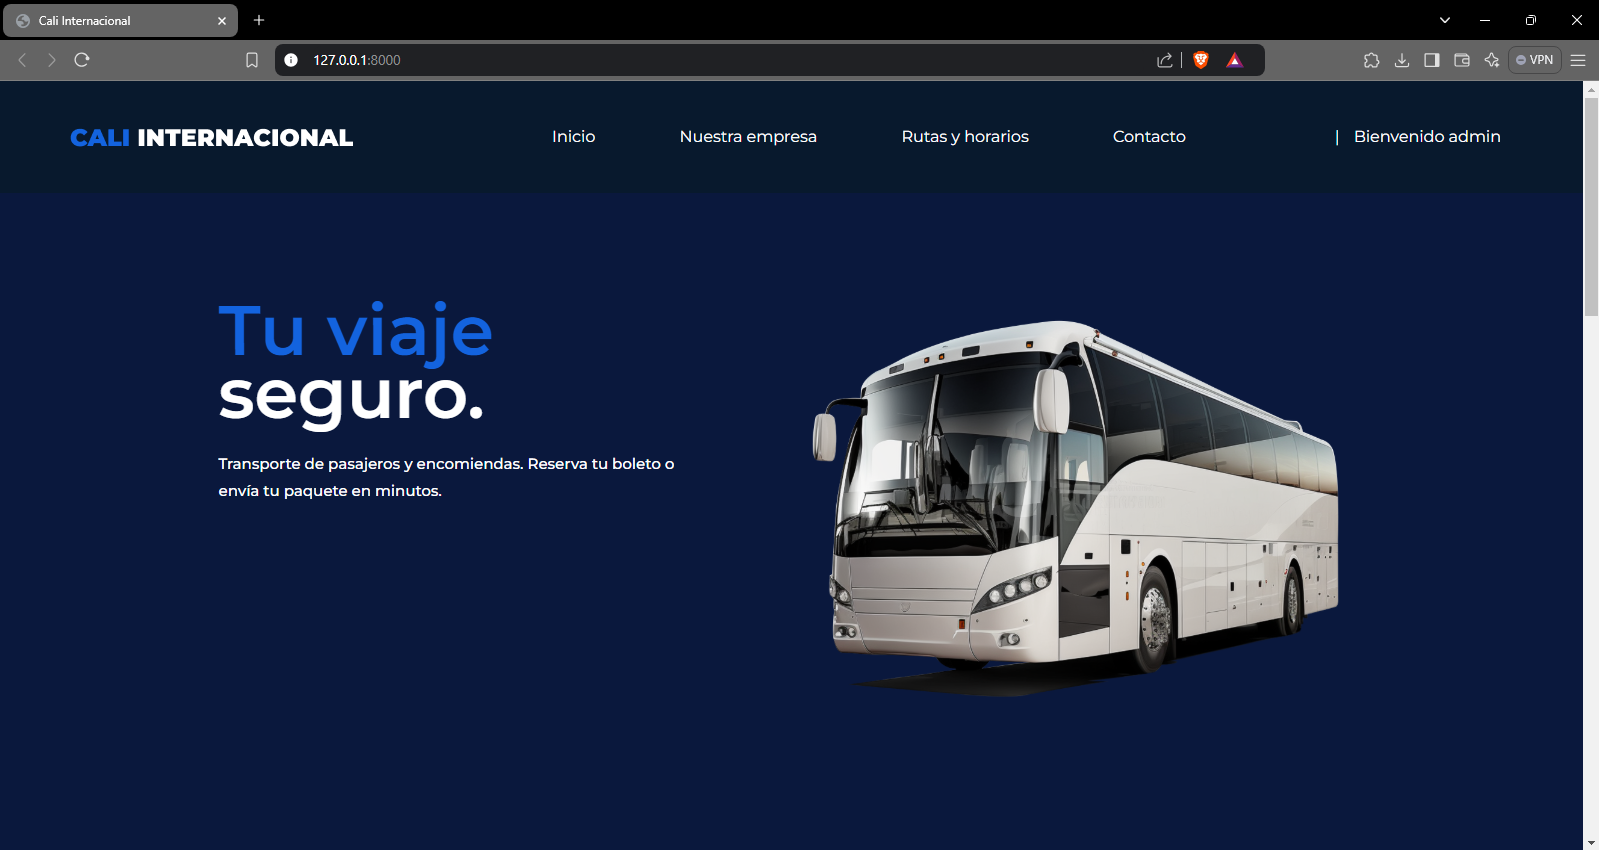
\includegraphics[width=0.9\textwidth]{imagenes/cap_3/Img_calibus/CALIBUS00.png} % Inserta una imagen
 	\begin{flushleft}
 		\begin{doublespace}
 			\hspace{1.20cm} \textbf{Nota.} Página principal de la web de Cali Internacional. % Nota al pie para esta figura
 		\end{doublespace}
 	\end{flushleft}
 	\vspace{-40pt} % hace que se acerque mas el texto
 	\label{fig:cali00} % Etiqueta para referencia cruzada
 \end{figure}
 
 %\vspace{-0.6cm} % Agregar 1 cm de espacio entre el párrafo y la figura
 
 En la figura \ref{fig:cali00} se ve la página web inicial de la Empresa de transportes Cali Internacional, posteriormente en la Figura \ref{fig:cali01} se observa la página de inicio de sesión.
 
 \vspace{0.3cm} % Agregar 1 cm de espacio entre el párrafo y la figura
 
 \begin{figure}[!h] % 'H' del paquete 'float' para mantener posición	
 	\caption[Inicio de sesión]
 	{\newline Inicio de sesión.} % Leyenda en la parte superior
 	\centering
 	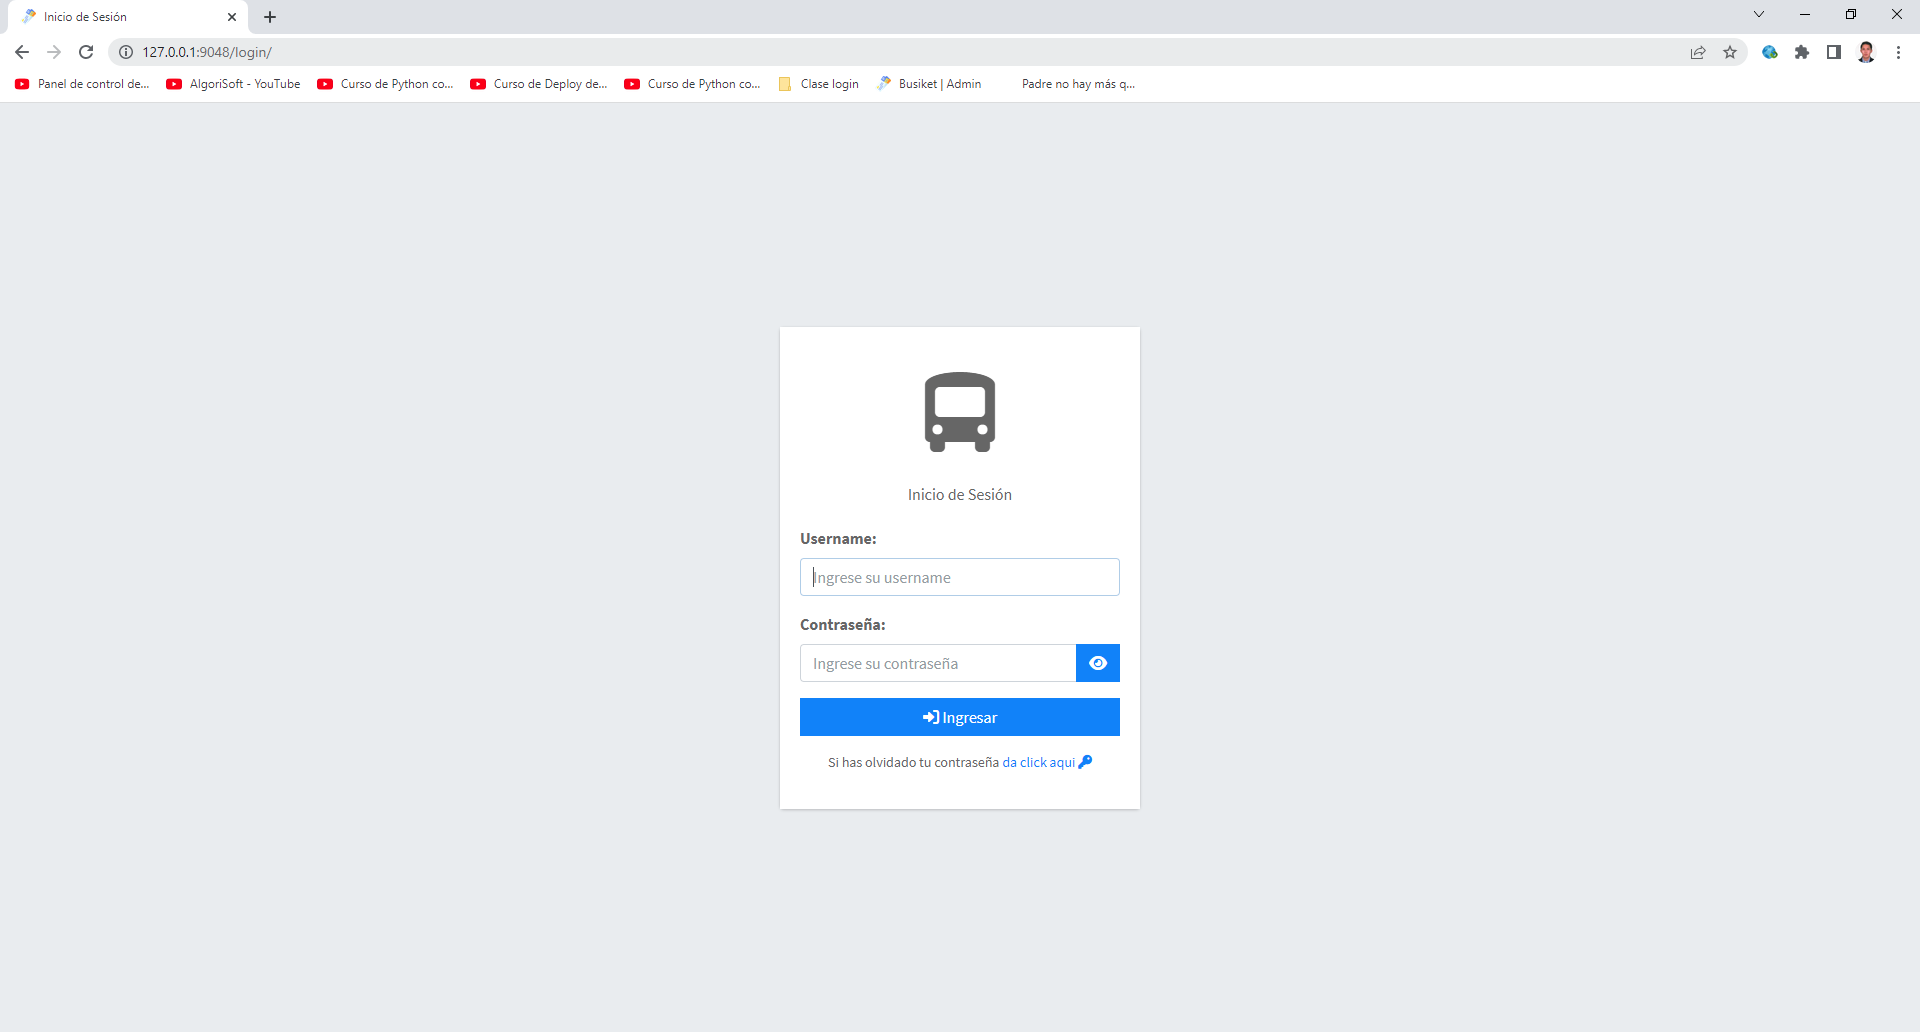
\includegraphics[width=0.75\textwidth]{imagenes/cap_3/Img_calibus/CALIBUS01.png} % Inserta una imagen
 	
 	\begin{flushleft}
 		\begin{doublespace}
 			\hspace{1.20cm} \textbf{Nota.} Interfaz de inicio de sesión para el acceso seguro al sistema. % Nota al pie para esta figura
 		\end{doublespace}
 	\end{flushleft}
 	\vspace{-40pt} % hace que se acerque mas el texto
 	\label{fig:cali01} % Etiqueta para referencia cruzada
 \end{figure}
 
 
 \begin{figure}[!h] % 'H' del paquete 'float' para mantener posición	
 	\caption[Panel principal del sistema]
 	{\newline Panel principal del sistema.} % Leyenda en la parte superior
 	\centering
 	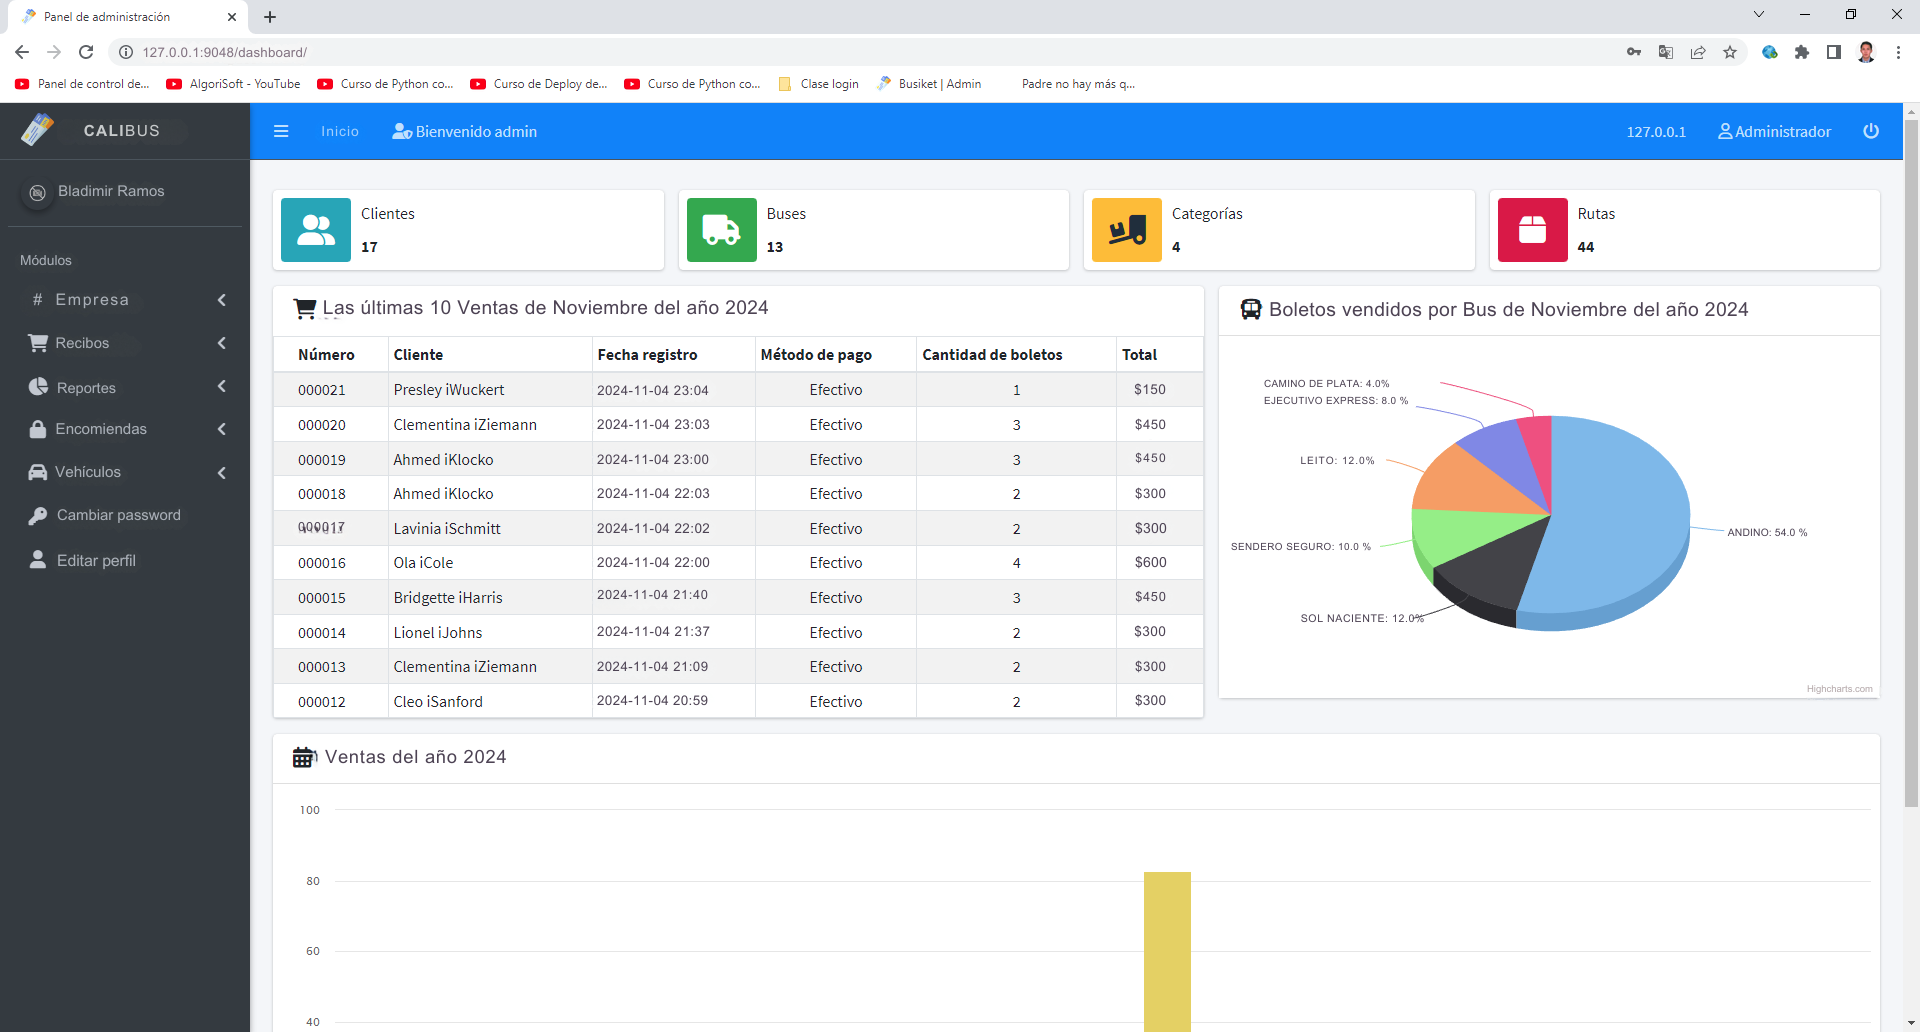
\includegraphics[width=0.75\textwidth]{imagenes/cap_3/Img_calibus/CALIBUS02.png} % Inserta una imagen
 	
 	\begin{flushleft}
 		\hspace{1.20cm} \textbf{Nota.} Panel principal que resume la información operativa y financiera. % Nota al pie para esta figura
 	\end{flushleft}
 	\vspace{-16pt}
 	\label{fig:cali02} % Etiqueta para referencia cruzada
 \end{figure}
 
 \vspace{-0.6cm} % Agregar 1 cm de espacio entre el párrafo y la figura
 
 En la figura \ref{fig:cali02} se ve el panel inciial del sistema.
 
 \vspace{0.3cm} % Agregar 1 cm de espacio entre el párrafo y la figura
 
 \begin{figure}[!h] % 'H' del paquete 'float' para mantener posición	
 	\caption[Creación de clientes]
 	{\newline Creación de clientes.} % Leyenda en la parte superior
 	\centering
 	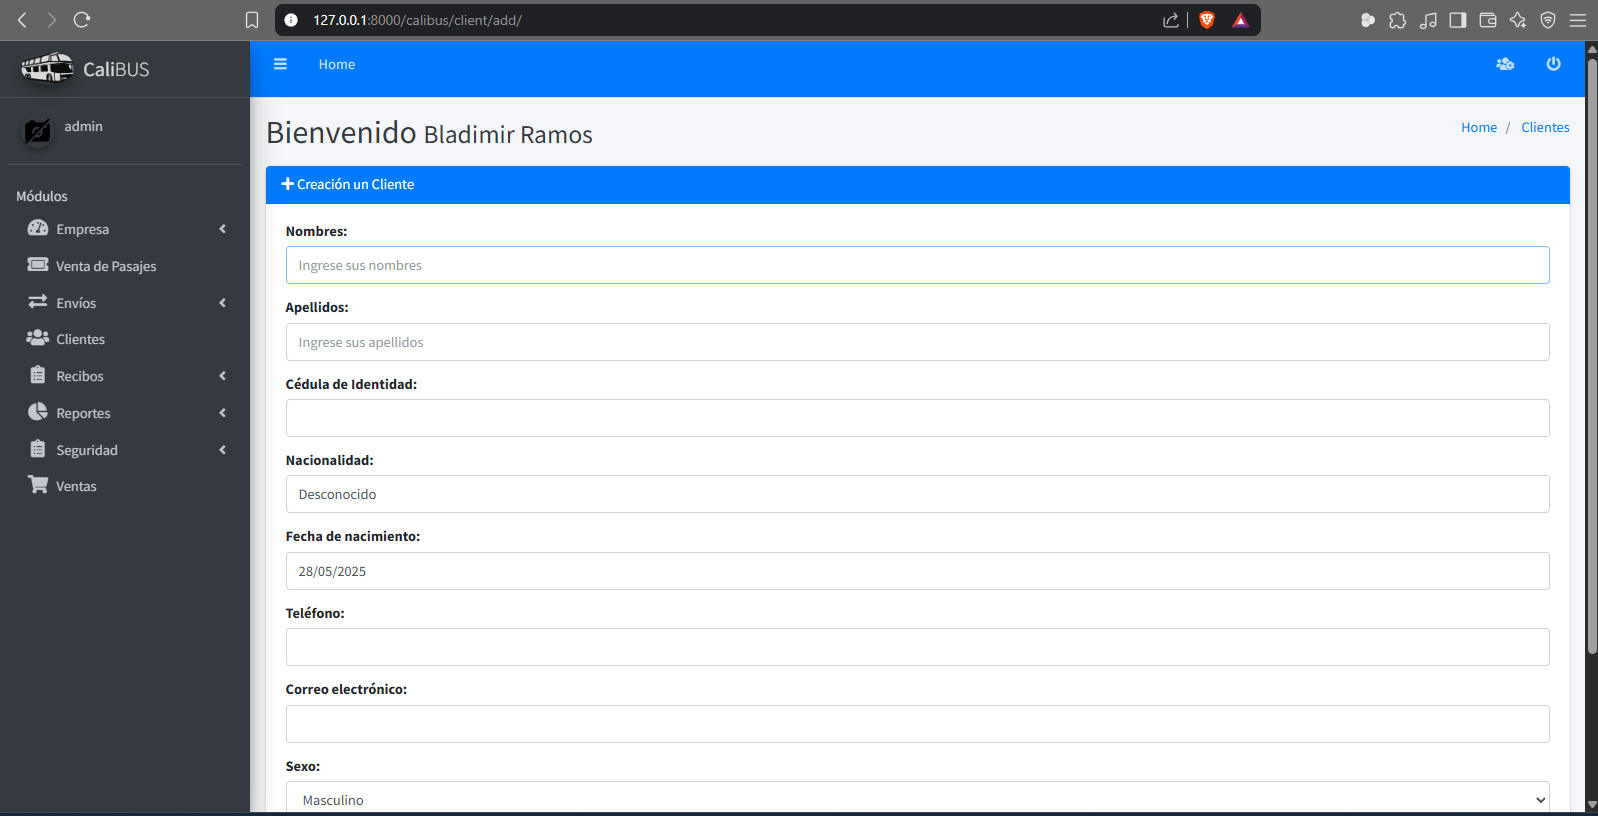
\includegraphics[width=0.85\textwidth]{imagenes/cap_3/Img_calibus/CALIBUS111.png} % Inserta una imagen
 	
 	\begin{flushleft}
 		\hspace{1.20cm} \textbf{Nota.} Pantalla de creación de clientes. % Nota al pie para esta figura
 	\end{flushleft}
 	\vspace{-16pt}
 	\label{fig:cali08} % Etiqueta para referencia cruzada
 \end{figure}
 
 En la Figura \ref{fig:cali08} y \ref{fig:cali09} se observa la gestión de los clientes tanto para la creación como el listado de los clientes que estan registrados.
 
 \begin{figure}[!h] % 'H' del paquete 'float' para mantener posición	
 	\caption[Listado de clientes]
 	{\newline Listado de clientes.} % Leyenda en la parte superior
 	\centering
 	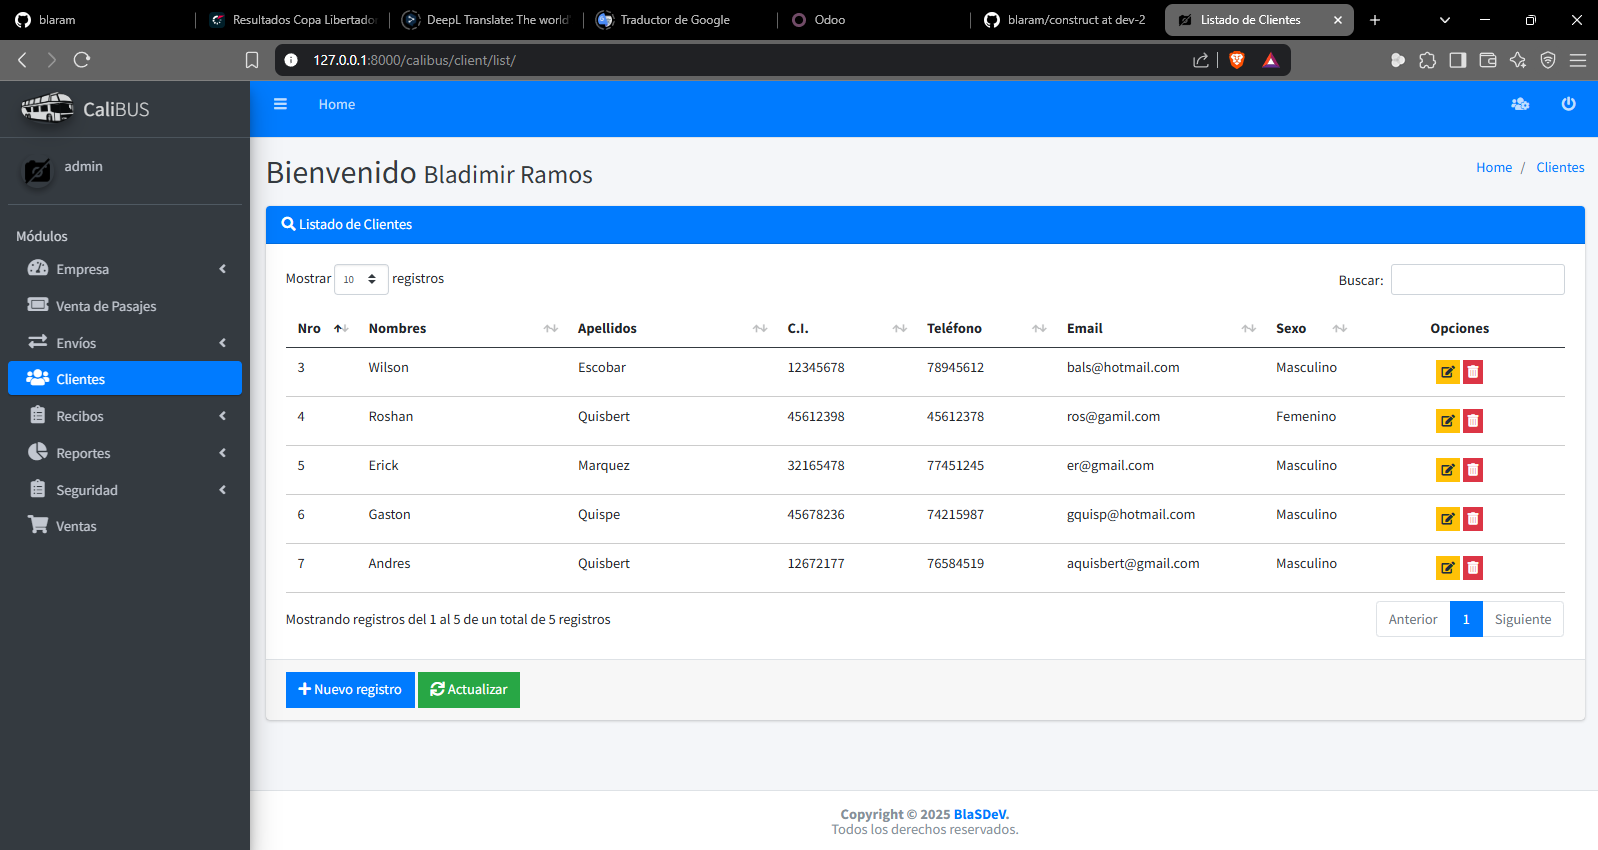
\includegraphics[width=0.85\textwidth]{imagenes/cap_3/Img_calibus/CALIBUS112.png} % Inserta una imagen
 	
 	\begin{flushleft}
 		\hspace{1.20cm} \textbf{Nota.} Vista con el listado de clientes registrados. % Nota al pie para esta figura
 	\end{flushleft}
 	\vspace{-16pt}
 	\label{fig:cali09} % Etiqueta para referencia cruzada
 \end{figure}
 
 \vspace{0.6cm} % Agregar 1 cm de espacio entre el párrafo y la figura
  
 \begin{figure}[!h] % 'H' del paquete 'float' para mantener posición	
 	\caption[Creación de un viaje]
 	{\newline Creación de un viaje.} % Leyenda en la parte superior
 	\centering
 	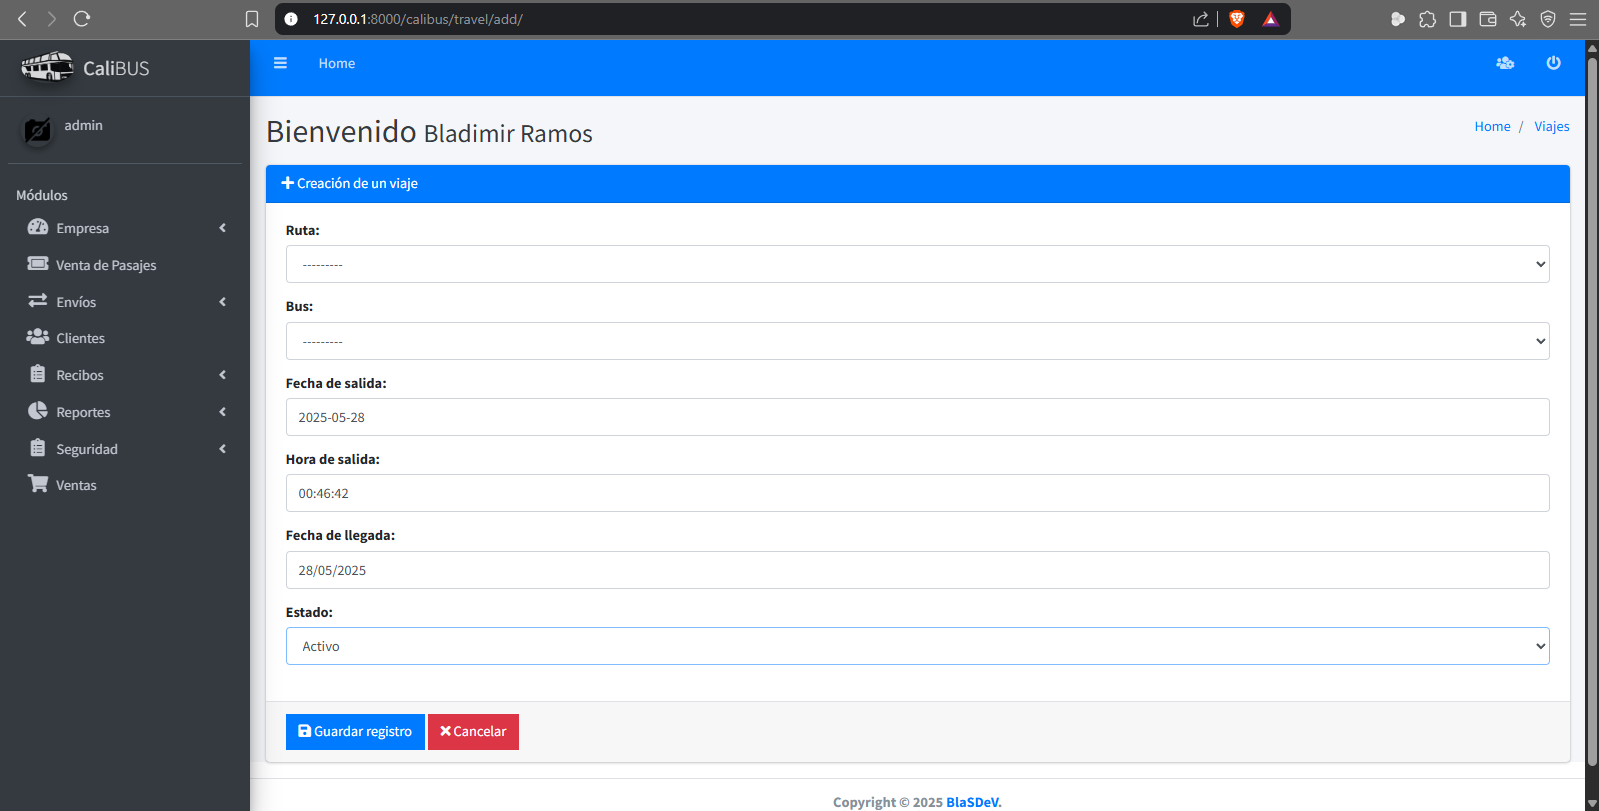
\includegraphics[width=0.83\textwidth]{imagenes/cap_3/Img_calibus/CALIBUS1112.png} % Inserta una imagen
 	
 	\begin{flushleft}
 		\hspace{1.20cm} \textbf{Nota.} Interfaz para la creación de viajes. % Nota al pie para esta figura
 	\end{flushleft}
 	\vspace{-16pt}
 	\label{fig:cali23} % Etiqueta para referencia cruzada
 \end{figure}
 
 En la figura \ref{fig:cali23} se ve la pantalla para la creación de los viajes, posteriormente en la Figura \ref{fig:cali18} se observa la pantalla para la venta de pasajes.
 
 \vspace{0.3cm} % Agregar 1 cm de espacio entre el párrafo y la figura 
 
 \begin{figure}[!h] % 'H' del paquete 'float' para mantener posición	
 	\caption[Venta o reserva de pasajes]
 	{\newline Venta o reserva de pasajes.} % Leyenda en la parte superior
 	\centering
 	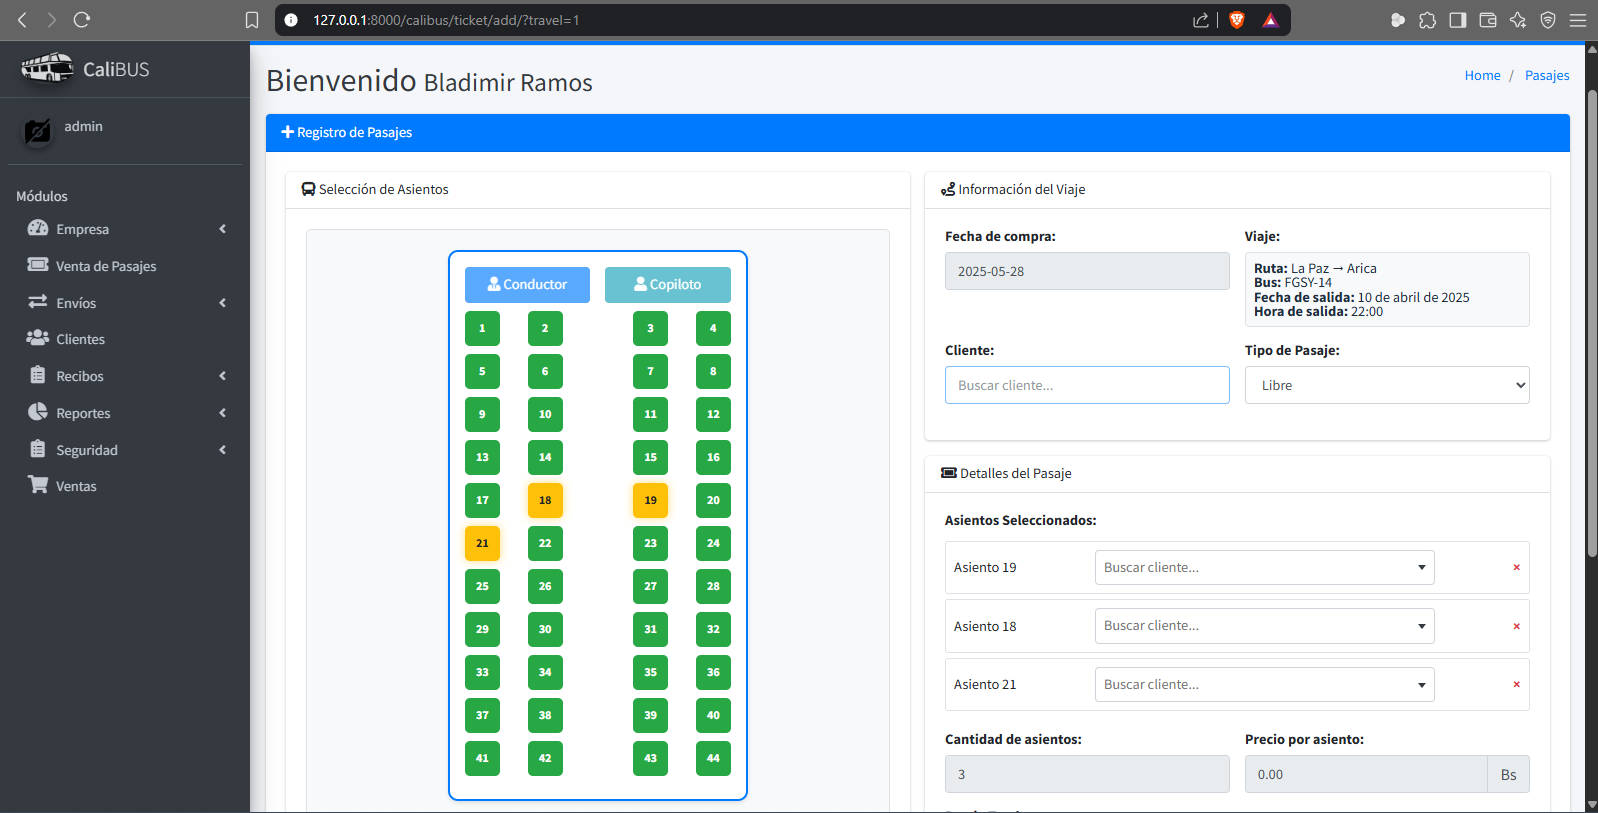
\includegraphics[width=0.83\textwidth]{imagenes/cap_3/Img_calibus/CALIBUS113.png} % Inserta una imagen
 	
 	\begin{flushleft}
 		\hspace{1.20cm} \textbf{Nota.} Pantalla para realizar la venta o reserva de pasajes, incluyendo selección de asiento y datos del pasajero. % Nota al pie para esta figura
 	\end{flushleft}
 	\vspace{-16pt}
 	\label{fig:cali18} % Etiqueta para referencia cruzada
 \end{figure}
 
 \vspace{-0.6cm} % Agregar 1 cm de espacio entre el párrafo y la figura
 
 En la figura \ref{fig:cali19} se observa la pantalla de registro de encomiendas, posteriormente en la Figura \ref{fig:cali20} se observa informe de ventas según una fecha específica.
 
 \vspace{0.3cm} % Agregar 1 cm de espacio entre el párrafo y la figura
 
 \begin{figure}[!h] % 'H' del paquete 'float' para mantener posición	
 	\caption[Gestión de encomiendas]
 	{\newline Gestión de encomiendas.} % Leyenda en la parte superior
 	\centering
 	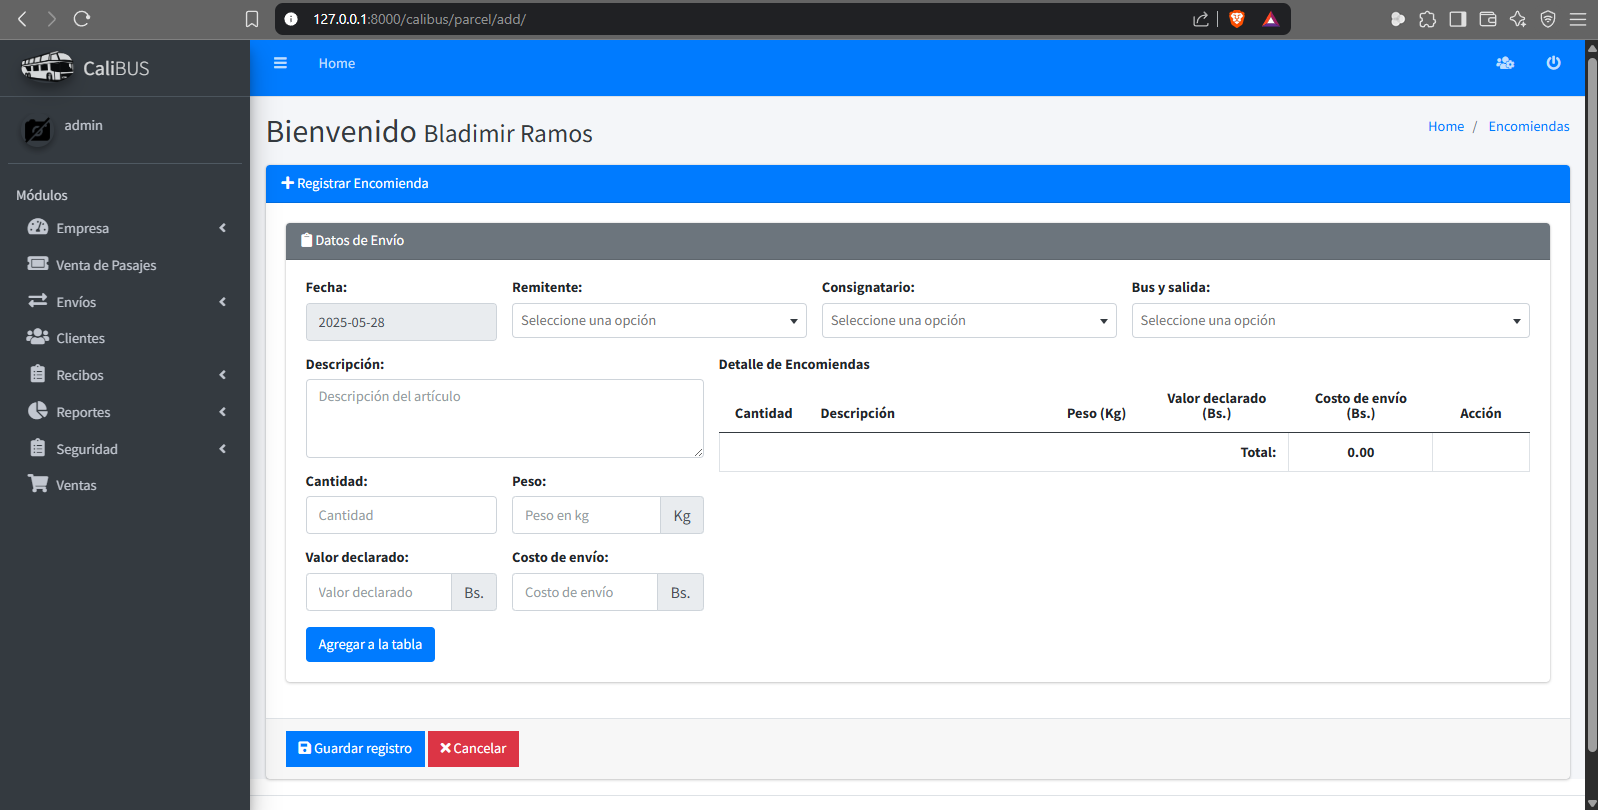
\includegraphics[width=0.83\textwidth]{imagenes/cap_3/Img_calibus/CALIBUS114.png} % Inserta una imagen
 	
 	\begin{flushleft}
 		\hspace{1.20cm} \textbf{Nota.} Módulo para el registro de las encomiendas. % Nota al pie para esta figura
 	\end{flushleft}
 	\vspace{-16pt}
 	\label{fig:cali19} % Etiqueta para referencia cruzada
 \end{figure} 
 
 \begin{figure}[!h] % 'H' del paquete 'float' para mantener posición	
 	\caption[Informe de ventas]
 	{\newline Informe de ventas.} % Leyenda en la parte superior
 	\centering
 	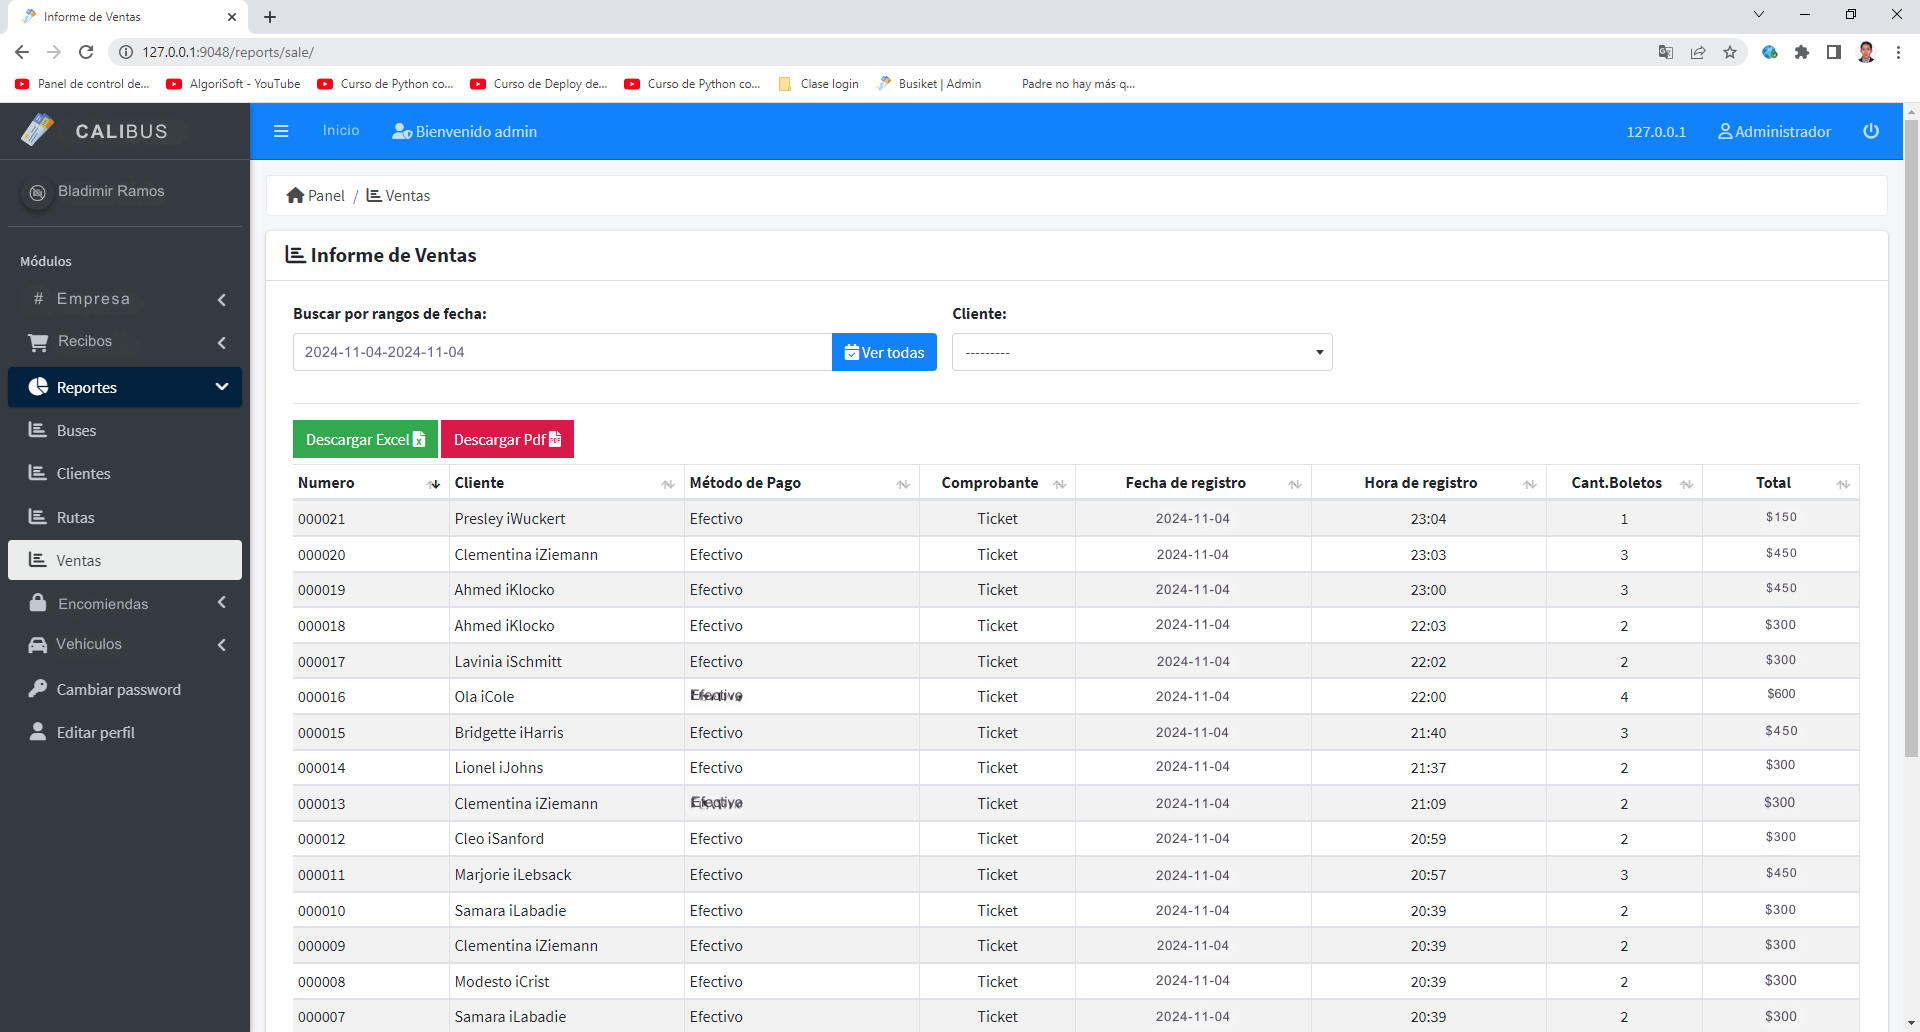
\includegraphics[width=0.83\textwidth]{imagenes/cap_3/Img_calibus/CALIBUS19.png} % Inserta una imagen
 	
 	\begin{flushleft}
 		\hspace{1.20cm} \textbf{Nota.} Informe de las ventas realizadas en el sistema. % Nota al pie para esta figura
 	\end{flushleft}
 	\vspace{-16pt}
 	\label{fig:cali20} % Etiqueta para referencia cruzada
 \end{figure}
 
 \vspace{-0.6cm} % Agregar 1 cm de espacio entre el párrafo y la figura
	
\section{RESULTADOS}
	La implementación del nuevo sistema ha permitido mejorar los tiempos asociados a las tareas del proceso operativo. Este avance se traduce en una mayor eficiencia en las operaciones diarias, ya que se reducen considerablemente los tiempos manuales involucrados en cada actividad.
	
	Además, la reducción de estos tiempos contribuye a minimizar errores humanos, lo que favorece la precisión y confiabilidad de los procesos dentro de la empresa. La automatización facilita que las tareas se realicen de forma más rápida y consistente.
	
	En las tablas 3.12, 3.13, 3.14, 3.15 y 3.16 se presentan comparativas de los tiempos promedio empleados en las principales actividades. Estas tablas reflejan claramente el impacto positivo del nuevo sistema frente a los métodos tradicionales, demostrando su efectividad en la simplificación y mejora continua de las operaciones diarias.
	
	\begingroup
		\onehalfspacing	
		\begin{longtable}{>{\centering\arraybackslash}m{3cm} >{\centering\arraybackslash}m{5cm} >{\centering\arraybackslash}m{4cm}}
			\caption[Tiempos para Registro de Usuarios]{\newline Tiempos para Registro de Usuarios} \label{tab:tabla3_12}\\
			\toprule
			\textbf{Nro} & \textbf{Sistema manual (min:seg)} & \textbf{Sistema web (min:seg)}\\
			\midrule
			\endfirsthead
			\bottomrule
			\endlastfoot
			
			% Aquí se colocan las filas de la tabla, por ejemplo:
			1 & 03:35 & 01:23 \\
			2 & 03:40 & 01:40 \\
			3 & 03:05 & 01:50 \\
			4 & 03:12 & 01:30 \\
			5 & 04:01 & 02:01 \\ \hline
			Promedio	& 03:31 & 01:41 \\ \hline
			Diferencia  &  & 01:50 \\ \hline
			Diferencia (\%) &   & 52.14\% \\
			
		\end{longtable}
		\vspace{-12pt}  % O el valor que necesites para ajustar
		% Nota personalizada fuera de `\caption*{}`
		\textbf{Nota}: Registro de tiempos promedio requeridos para completar el proceso de creación de usuarios en el sistema.
	\endgroup
	
	\begingroup
		\onehalfspacing	
		\begin{longtable}{>{\centering\arraybackslash}m{3cm} >{\centering\arraybackslash}m{5cm} >{\centering\arraybackslash}m{4cm}}
			\caption[Tiempos para Venta de Pasajes]{\newline Tiempos para Venta de Pasajes} \label{tab:tabla3_13}\\
			\toprule
			\textbf{Nro} & \textbf{Sistema manual (min:seg)} & \textbf{Sistema web (min:seg)}\\
			\midrule
			\endfirsthead
			\bottomrule
			\endlastfoot	
			% Aquí se colocan las filas de la tabla, por ejemplo:
			1 & 04:10 & 01:30 \\	
			2 & 04:39 & 01:20 \\
			3 & 05:16 & 01:26 \\
			4 & 04:28 & 01:10 \\
			5 & 04:36 & 01:45 \\ \hline
			Promedio	& 04:38 & 01:26 \\ \hline
			Diferencia  &  & 03:12 \\ \hline
			Diferencia (\%) &   & 69\% \\
			
		\end{longtable}
		\vspace{-12pt}  % O el valor que necesites para ajustar
		% Nota personalizada fuera de `\caption*{}`
		\textbf{Nota}: Medición de tiempos promedio requeridos para completar el proceso de creación de usuarios en el sistema.
	\endgroup
	
	\begingroup
		\onehalfspacing	
		\begin{longtable}{>{\centering\arraybackslash}m{3cm} >{\centering\arraybackslash}m{5cm} >{\centering\arraybackslash}m{4cm}}
			\caption[Tiempos para Reserva de Pasajes]{\newline Tiempos para Reserva de Pasajes} \label{tab:tabla3_14}\\
			\toprule
			\textbf{Nro} & \textbf{Sistema manual (min:seg)} & \textbf{Sistema web (min:seg)}\\
			\midrule
			\endfirsthead
			\bottomrule
			\endlastfoot			
			% Aquí se colocan las filas de la tabla, por ejemplo:
			1 & 02:15 & 00:58 \\
			2 & 02:01 & 00:56 \\
			3 & 02:21 & 00:49 \\
			4 & 02:32 & 00:52 \\
			5 & 02:03 & 00:56 \\ \hline
			Promedio	& 02:14 & 00:54 \\ \hline
			Diferencia  &  & 01:20 \\ \hline
			Diferencia (\%) &   & 59.67\% \\
			
		\end{longtable}
		\vspace{-12pt}  % O el valor que necesites para ajustar
		% Nota personalizada fuera de `\caption*{}`
		\textbf{Nota}: Resultados de los tiempos de respuesta para completar la reserva de pasajes en distintas pruebas.
	\endgroup
	
	\begingroup
		\onehalfspacing	
	\begin{longtable}{>{\centering\arraybackslash}m{3cm} >{\centering\arraybackslash}m{5cm} >{\centering\arraybackslash}m{4cm}}
		\caption[Tiempos para Registro de Encomiendas]{\newline Tiempos para Registro de Encomiendas} \label{tab:tabla3_15}\\
		\toprule
		\textbf{Nro} & \textbf{Sistema manual (min:seg)} & \textbf{Sistema web (min:seg)}\\
		\midrule
		\endfirsthead
		\bottomrule
		\endlastfoot		
		% Aquí se colocan las filas de la tabla, por ejemplo:
		1 & 04:12 & 02:23 \\
		2 & 05:01 & 02:11 \\
		3 & 04:26 & 02:02 \\
		4 & 04:45 & 02:03 \\
		5 & 05:15 & 02:43 \\ \hline
		Promedio	& 04:44 & 02:16 \\ \hline
		Diferencia  &  & 02:27 \\ \hline
		Diferencia (\%) &   & 51.94\% \\
		
	\end{longtable}
	\vspace{-12pt}  % O el valor que necesites para ajustar
	% Nota personalizada fuera de `\caption*{}`
	\textbf{Nota}: Tiempos necesarios para registrar una encomienda desde su ingreso hasta la confirmación.
	\endgroup
	
	\begingroup
		\onehalfspacing	
	\begin{longtable}{>{\centering\arraybackslash}m{3cm} >{\centering\arraybackslash}m{5cm} >{\centering\arraybackslash}m{4cm}}
		\caption[Tiempos para Generar Reportes]{\newline Tiempos para Generar Reportes} \label{tab:tabla3_16}\\
		\toprule
		\textbf{Nro} & \textbf{Sistema manual (min:seg)} & \textbf{Sistema web (min:seg)}\\
		\midrule
		\endfirsthead	
		\bottomrule
		\endlastfoot
		% Aquí se colocan las filas de la tabla, por ejemplo:
		1 & 20:14 & 02:03 \\
		2 & 21:10 & 02:22 \\
		3 & 19:56 & 02:01 \\
		4 & 19:22 & 01:59 \\
		5 & 23:45 & 01:39 \\ \hline
		Promedio	& 20:53 & 02:01 \\ \hline
		Diferencia  &  & 18:53 \\ \hline
		Diferencia (\%) &   & 90.36\% \\
		
	\end{longtable}
	\vspace{-12pt}  % O el valor que necesites para ajustar
	% Nota personalizada fuera de `\caption*{}`
	\textbf{Nota}: Evaluación de los tiempos requeridos para le generación de reportes por parte del sistema.
	\endgroup

	\begingroup
	\onehalfspacing	
	\begin{longtable}{>{\centering\arraybackslash}m{3.5cm} >{\centering\arraybackslash}m{3.5cm} >{\centering\arraybackslash}m{3cm} >{\centering\arraybackslash}m{2.5cm} >{\centering\arraybackslash}m{2.5cm}}
		\caption[Resumen tiempos de actividades]{\newline Resumen tiempos de actividades} \label{tab:tabla3_17}\\
		\toprule
		\textbf{Actividad} & \textbf{Sistema manual (min:seg)} & \textbf{Sistema web (min:seg)} & \textbf{Diferencia} & \textbf{Promedio} \% \\
		\midrule
		\endfirsthead
		\bottomrule
		\endlastfoot	
		% Aquí se colocan las filas de la tabla, por ejemplo:
		Registro de usuarios 	& 03:31 & 01:41 & 01:50 & 52.14 \\
		Ventas de pasajes 		& 04:38 & 01:26 & 03:12 & 68.97 \\
		Reserva de pasajes 		& 02:14 & 00:54 & 01:20 & 59.67 \\
		Registro de encomiendas & 04:44 & 02:16 & 02:27 & 51.94 \\
		Generar reportes 		& 20:53 & 02:01 & 18:53 & 90.36 \\ \hline
		Promedio				&       &       &       & 64.62 \\
		
	\end{longtable}
	\vspace{-12pt}  % O el valor que necesites para ajustar
	% Nota personalizada fuera de `\caption*{}`
	\textbf{Nota}: Comparativo general de los tiempos empleados en cada una de las actividades principales del sistema.
	\endgroup

	\vspace{0.3cm} % Agregar 1 cm de espacio entre el párrafo y la figura
	
	\begin{figure}[h] % 'H' del paquete 'float' para mantener posición	
			\caption[Comparación de mejora de tiempos]
			{\newline Comparación de mejora de tiempos.} % Leyenda en la parte superior
			\centering
			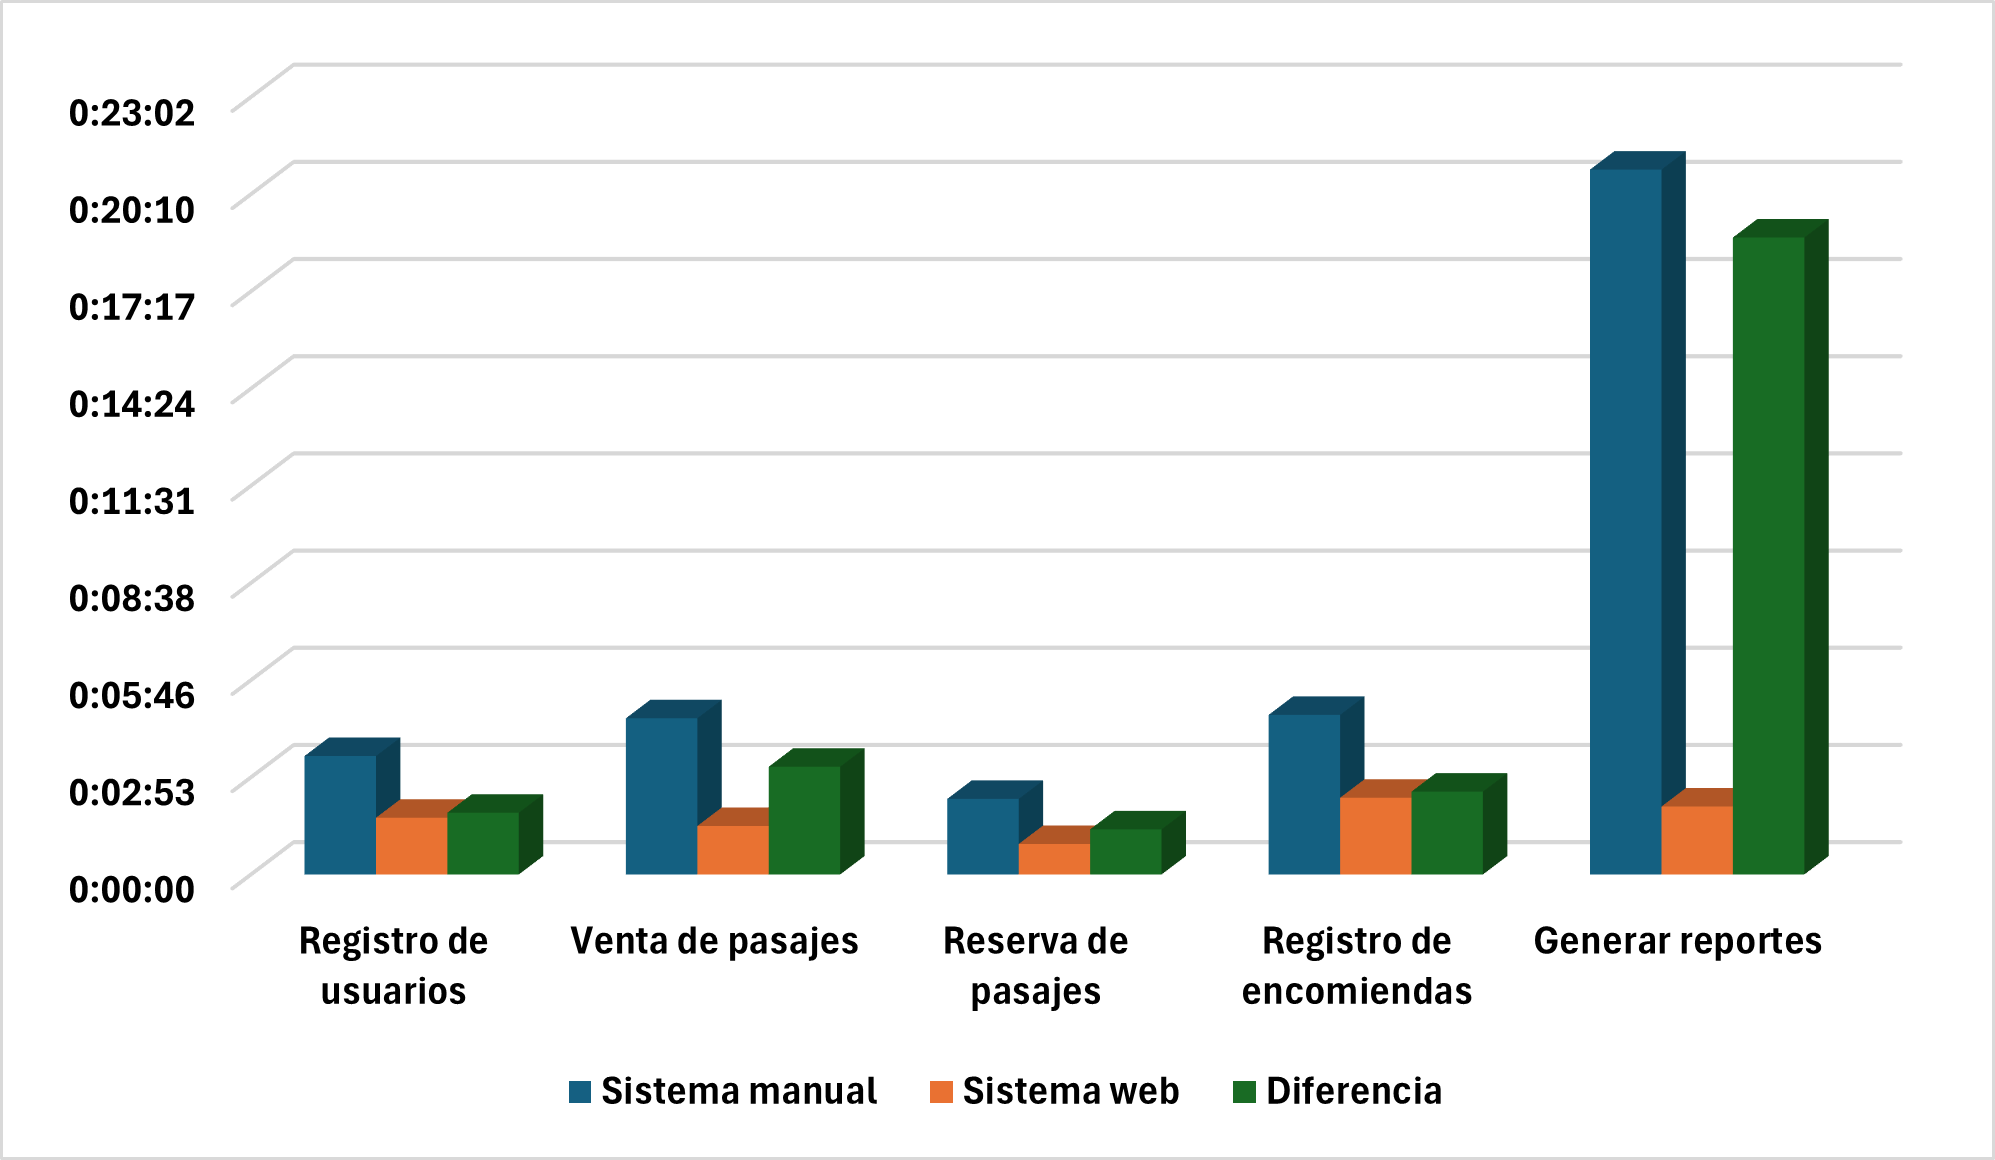
\includegraphics[width=0.8\textwidth]{imagenes/cap_3/Resultados.png} % Inserta una imagen
			
		\begin{flushleft}
			\begin{doublespace}
				\hspace{1.20cm} \textbf{Nota.} La figura muestra la diferencia de tiempos promedio antes y despues de la implementación del sistema. % Nota al pie para esta figura
			\end{doublespace}
		\end{flushleft}
		\vspace{-16pt} % hace que se acerque mas el texto
		\label{fig:figura_resultados} % Etiqueta para referencia cruzada
	\end{figure}
	
	Dados los resultados de la tabla \ref{tab:tabla3_17} y la figura \ref{fig:figura_resultados} se evidencia que la implementación del nuevo sistema permite mejorar los procesos operativos, logrando una reducción promedio del 64.62 por ciento en los tiempos de ejecución de actividades, este ahorro representa una transformación significativa en la mejora dela empresa, ya que los procesos manuales, que antes eran tediosos y propensos a errores, han sido sustituidos por un sistema automatizado que prioriza la rapidez. Este avance no solo mejora la experiencia del cliente al reducir los tiempos de espera, sino que también libera recursos para que el personal pueda enfocarse en actividades de mayor valor, fortaleciendo la posición competitiva de la empresa en el mercado.